\documentclass[11pt,a4paper]{article}
\usepackage[T1]{fontenc}
\usepackage[utf8]{inputenc}
\usepackage{lmodern}
\usepackage[a4paper,margin=23mm,headheight=15pt]{geometry}
\usepackage{microtype}
\usepackage{xcolor,graphicx,booktabs,longtable,tabularx,array}
\usepackage{enumitem,listings,fancyhdr,titlesec,needspace,etoolbox}
\usepackage{tikz}
\usetikzlibrary{arrows.meta,positioning,fit,backgrounds,shapes.geometric}
\usepackage{xurl}
\usepackage[colorlinks=true,linkcolor=blue!45!black,urlcolor=blue!45!black,citecolor=blue!45!black,pdfborder={0 0 0}]{hyperref}
\hypersetup{hypertexnames=false,pdftitle={Object Storage and Fine-Grained Access Control: Specification 2.6.1},pdfauthor={Engineering design specification},pdfsubject={Storage-first Go platform with shared authorization; MCP as a subsequent service}}
\definecolor{ink}{HTML}{163447}
\definecolor{accent}{HTML}{187F86}
\definecolor{pale}{HTML}{EEF4F6}
\titleformat{\section}{\Large\bfseries\color{ink}}{\thesection}{0.7em}{}
\titleformat{\subsection}{\large\bfseries\color{ink}}{\thesubsection}{0.7em}{}
\titleformat{\subsubsection}{\normalsize\bfseries}{\thesubsubsection}{0.7em}{}
\setlength{\parindent}{0pt}
\setlength{\parskip}{5pt}
\setlength{\emergencystretch}{3em}
\setlength{\tabcolsep}{5pt}
\renewcommand{\arraystretch}{1.17}
\setlist{nosep,leftmargin=1.5em,topsep=4pt}
\pagestyle{fancy}
\fancyhf{}
\fancyhead[L]{\small\color{ink}OBJECT STORAGE AND ACCESS CONTROL}
\fancyhead[R]{\small Specification 2.6.1 (draft)}
\fancyfoot[L]{\small 31 October 2026}
\fancyfoot[R]{\small\thepage}
\renewcommand{\headrulewidth}{0.4pt}
\newcommand{\must}{\textbf{MUST}}
\newcommand{\mustnot}{\textbf{MUST NOT}}
\newcommand{\should}{\textbf{SHOULD}}
\newcommand{\term}[1]{\textbf{#1}}
\newcommand{\code}[1]{{\small\nolinkurl{#1}}}
\newcommand{\arrowto}{$\rightarrow$}
\newcommand{\rr}[1]{\hyperlink{req:#1}{#1}}
\newcommand{\reqtag}[2]{{\footnotesize\color{accent}(#1\,$\cdot$\,#2)}}
\newcommand{\req}[4]{\par\noindent\hypertarget{req:#1}{\textbf{[#1]}}\ #4\ \reqtag{#2}{#3}\par}
\newcommand{\reqn}[4]{\par\noindent\hypertarget{req:#1}{\textbf{[#1]}}\textsuperscript{\color{accent}\tiny NEW}\ #4\ \reqtag{#2}{#3}\par}
\newcommand{\testrow}[4]{\hypertarget{test:#1}{\textbf{#1}} & #2 & #3 & #4\\}
\lstset{basicstyle=\ttfamily\small,backgroundcolor=\color{pale},frame=single,rulecolor=\color{pale},breaklines=true,columns=fullflexible,keepspaces=true,showstringspaces=false,tabsize=2,xleftmargin=5pt,xrightmargin=5pt,aboveskip=8pt,belowskip=8pt}
\newcolumntype{P}[1]{>{\raggedright\arraybackslash}p{#1}}
\newcolumntype{Y}{>{\raggedright\arraybackslash}X}
\BeforeBeginEnvironment{lstlisting}{\Needspace{12\baselineskip}}
\pretocmd{\subsection}{\Needspace{7\baselineskip}}{}{}
\begin{document}
\begin{titlepage}
\vspace*{15mm}
{\color{accent}\large ENGINEERING SPECIFICATION\par}
\vspace{8mm}
{\color{ink}\Huge\bfseries Object Storage and\par Fine-Grained Access Control\par}
\vspace{7mm}
{\LARGE Encrypted Go storage and shared authorization,\par with MCP built as a subsequent service\par}
\vspace{15mm}
\begin{tabularx}{\textwidth}{@{}P{34mm}Y@{}}
\toprule
Version & 2.6.1 (revised draft), 31 October 2026. Supersedes 2.6, which it corrects only in the grant targets and grantable actions of share grants. Version 2.6 superseded 2.5 and added decision D-12: every payload is encrypted, by the platform under decision-bound keys by default or by the client in buckets that opt into client mode, and share grants let a user name a reader where policy honors them. Earlier changes are recorded in Appendix~\ref{app:review}.\\
Status & Specification and document checks only. Implementation, cryptographic interoperability and qualification remain open; scenario descriptions alone are not passing evidence.\\
Structure & R1: encrypted object storage in server or client mode, fine-grained access, decision-bound key release, recipient envelopes, share grants and document/text units. R2: a separate MCP service, with compatible decrypting clients for client-mode content; optional client-side model/tool services. R3: S3 and optional custom replication. Requirements retain stable identifiers, phases and verification links.\\
Core language & Go; one module; roles built from role-specific entrypoints.\\
Open decisions & Phase 0 decisions D-04 to D-11 and D-13 (Section~\ref{sec:decisions}) must be closed before the work they gate; D-01 to D-03 and D-12 are decided.\\
Deliverables & Standalone LaTeX source and PDF; companion sources with scenarios, concrete fixtures, consistency checks and implementation-profile notes.\\
\bottomrule
\end{tabularx}\par
\vspace{8mm}
\textbf{Central principle.} Build secure object storage and one fine-grained access-control authority first: deny by default, encrypt every payload, and release content or keys only to authorized callers. By default the platform encrypts and decrypts under keys that only a fresh decision releases; a bucket that opts into client mode keeps decryption on authorized clients. MCP then connects to those services and exposes the same resources under the same permissions. Documents and text units are storage resources in their own right. Plaintext and ciphertext delivery, key release, encrypted key envelopes and later tool calls follow the same authority; no protocol grants a parallel route around it.
\vfill
The component prefix \texttt{fga} is a placeholder, not a product or trademark selection. All described modules and APIs are proposed project code unless identified as external dependencies. Items carried over from version 1.3 that this revision could not re-verify (version pins, commit hashes, URLs, upstream license terms) are listed in Appendix~\ref{app:unverified}.
\end{titlepage}
\pagenumbering{roman}{\small\setlength{\parskip}{0pt}\tableofcontents}\clearpage\pagenumbering{arabic}

\setcounter{section}{-1}
\section{Overview, guarantees and threat model}\label{sec:overview}
\subsection{Product statement and scope boundary}
The platform decides and enforces who may do what to which resource. It serves people, agents acting for people, tools, MCP clients and HTTP clients, and in a later release S3 clients. Every protected operation is an explicit action on a resource, evaluated with trusted identity, delegation, resource state and execution context. An enforcement point binds the result to the actual operation. Document text, search, model submission and key release use the same decision model.

``Access for everything'' means a common resource/action vocabulary and a small adapter contract. It does not mean that one server controls arbitrary operating-system calls, third-party credentials, databases or files outside its enforcement paths. A resource is protected only when every relevant access route is mediated or independently restricted.

\reqn{OVR-001}{P0}{REV}{Every release publishes an enforcement coverage matrix that lists each access route to protected resources (adapter, operation, resource type, action, mediation point, verifying test). A route that is absent from the matrix \mustnot\ be described as protected.}
\reqn{OVR-002}{P0}{LINT}{Each threat in Table~\ref{tab:threats} maps to at least one requirement and one test, and each guarantee in Table~\ref{tab:guarantees} maps to at least one requirement and one test. The specification check fails when a mapping is missing or names an undefined identifier.}
\reqn{OVR-003}{P0}{REV}{Product documentation and external claims \mustnot\ state more than the guarantees in Table~\ref{tab:guarantees} and \must\ repeat the non-guarantees in Table~\ref{tab:nonguarantees} wherever revocation, model-output control, encryption or storage durability is described.}

\textbf{Out of scope for this specification:} attribute-based and proxy re-encryption, erasure-coded storage, compiling policy into database queries, general file-content redaction, FTP/SFTP, S3 Select, tiering, site replication, and mediation of unrestricted local shells or direct local file reads.

\subsection{Releases and exit gates}\label{sec:releases}
The original design bundled five products. This revision orders them by risk and dependency. A release is accepted only when its exit tests (Section~\ref{sec:testmatrix}) pass; later releases do not weaken earlier gates.
\begin{longtable}{@{}P{0.08\textwidth}P{0.50\textwidth}P{0.30\textwidth}@{}}
\toprule Phase & Delivers & Exit tests\\\midrule\endhead
R1-A & \textbf{Decision core.} Identity and delegation, resource registry, policy evaluation in the production profile, Decide/DecideBatch with signed decisions, policy releases, catalog, audit outbox. Part~1. & T-01, T-02, T-03, T-13 (admission cases), T-14, T-15 (audit cases), T-19, T-20\\
R1-B & \textbf{Enforcement.} Tool executor, registry, approvals, reservations, invocation state machine, one real connector. Part~2. & T-04, T-05\\
R1-C & \textbf{Content, documents and MCP over our own single-node store.} Content service, publication protocol, labels, units, disclosure, search, derived outputs, context high-water mark, control-plane availability. Parts~2 (MCP) and~3. & T-06, T-08, T-09, T-13, T-15, T-16, T-18, T-21, T-22\\
R2 & \textbf{Key custody.} Envelope encryption, key broker, KMS provider, recipient registry, HPKE export. Part~4. & T-10, T-11, T-12, T-13, T-22\\
R3 & \textbf{S3 and replicated storage.} SigV4 profile, S3 handlers, replicated blob backend, repair, evacuation. Part~5. & T-07, T-08, T-15, T-17, T-18\\
\bottomrule
\end{longtable}
Phase P0 labels process requirements that apply from the first commit. In R1, at-rest protection of blobs comes from the host's disk encryption, and the platform does not advertise per-unit cryptographic separation; that claim starts with R2. Everything runs locally for now; the multi-domain topology is a later target.

R1-A, R1-B and R1-C are subphases of one release: none is deployed to production on its own (\rr{GATE-003}). Where a test is shared across subphases, its cases are assigned to the earliest subphase whose requirements claim it as their verification (Table~\ref{tab:tests}), and the specification check rejects a requirement whose test first applies in a later phase.

\subsection{Guarantees and non-guarantees}\label{sec:guarantees}
Table~\ref{tab:guarantees} is the complete list of what the platform promises. Each row is conditional on its requirements being implemented and its tests passing. Table~\ref{tab:nonguarantees} lists limits that recur throughout the document; they are stated here once.
\begin{longtable}{@{}P{0.07\textwidth}P{0.46\textwidth}P{0.24\textwidth}P{0.12\textwidth}@{}}
\caption{Guarantees}\label{tab:guarantees}\\
\toprule ID & Guarantee & Requirements & Tests\\\midrule\endfirsthead
\toprule ID & Guarantee & Requirements & Tests\\\midrule\endhead
G-01 & Fail closed. A protected operation runs only on an explicit, complete \code{ALLOW} bound to the exact operation. & \rr{DEC-002}, \rr{ENF-001}, \rr{ENF-003} & T-01, T-04\\
G-02 & One decision, many routes. The same normalized request gets the same business decision through every adapter. & \rr{RES-002}, \rr{RES-003}, \rr{CNT-001}, \rr{MCP-002} & T-01, T-06\\
G-03 & Fresh authority. A stale policy bundle, stale identity or delegation revision, or expired decision never authorizes; authority is rechecked at admission and at the irreversible checkpoint. & \rr{DEC-005}, \rr{DEC-006}, \rr{REL-003} & T-13, T-14\\
G-04 & Platform ceilings. No principal, role or tenant-scope policy result can override a platform ceiling or tenant isolation. & \rr{POL-007}, \rr{DAT-001} & T-01, T-02\\
G-05 & Bound approvals and budgets. Approvals and reservations are single-use, bound to the exact operation, and consumed atomically. & \rr{APR-001}, \rr{APR-002}, \rr{APR-004} & T-04, T-05\\
G-06 & No assumed outcomes. An external effect with an unknown result is held as \code{UNKNOWN} and resolved by a recorded action; it is never treated as success or failure. & \rr{INV-003}, \rr{INV-006}, \rr{INV-007} & T-05\\
G-07 & Unit-level disclosure. A denied unit does not reach a recipient through any supported disclosure route (search, read, citation, model context, derived output). & \rr{DSC-001}, \rr{DSC-002}, \rr{DRV-002} & T-09\\
G-08 & Durable evidence. Decisions, key releases, mutations and approval consumption leave audit records that do not silently drop. & \rr{AUD-001}, \rr{AUD-002} & T-15\\
\bottomrule
\end{longtable}
\begin{longtable}{@{}P{0.07\textwidth}P{0.55\textwidth}P{0.27\textwidth}@{}}
\caption{Non-guarantees}\label{tab:nonguarantees}\\
\toprule ID & Limit & Requirements\\\midrule\endfirsthead
\toprule ID & Limit & Requirements\\\midrule\endhead
N-01 & Revocation does not recall bytes already emitted, exported keys, retained plaintext or context already received by a model provider. Exposure on a live stream is bounded by the stream lease. & \rr{KEY-010}, \rr{CNT-008}\\
N-02 & No guarantee about what a model infers, says or sends. Cross-tool flow is constrained only for mediated tools, through the execution-context high-water mark, and only for runtimes that preserve their context lifetime; unmediated egress and content that reaches the agent by other routes are not covered. & \rr{FLW-001}, \rr{FLW-003}, \rr{FLW-005}, \rr{FLW-008}\\
N-03 & Server-managed encryption does not exclude storage-service operators from plaintext. It protects against reading storage disks and backups. & \rr{CRY-001}\\
N-04 & No defence against a host operator who can replace the running software, or against a holder of valid KMS credentials beyond key-release audit. & \rr{ADM-003}, \rr{KEY-007}\\
N-05 & No exactly-once guarantee across arbitrary external APIs. & \rr{INV-005}\\
N-06 & No claim that a policy expresses its owner's intent. The platform enforces what the policy says and reports effect changes on the conformance corpus. & \rr{REL-005}\\
N-07 & No regulatory WORM or Object Lock claim, no universal document parsing, and no claim that default S3 client settings work. & \rr{PUB-009}, \rr{DOC-004}, \rr{S3P-001}\\
N-08 & R1 stores blobs on one node. Losing that node loses blobs written since the last backup, so R1 makes no zero-loss claim for blob content. & \rr{BKD-002}, \rr{AVL-005}\\
\bottomrule
\end{longtable}

\subsection{Threat model}\label{sec:threats}
\textbf{Assets.} A1 protected content and plaintext; A2 keys and key material; A3 policy bundles, identity, delegation and other authority state; A4 approvals, budgets and invocation state; A5 audit evidence; A6 credentials for downstream tools.

\textbf{Adversaries.} E1 malicious or curious tenant user; E2 manipulated agent or model (prompt injection, hostile retrieved content); E3 compromised or malicious tool server, connector or downstream service; E4 compromised gateway or content-service process; E5 reader of storage disks or backups; E6 holder of broker or KMS credentials; E7 over-privileged or malicious administrator, including a policy author; E8 network attacker; E9 recipient that retains exported keys or plaintext. A host operator able to replace the running software (E10) is out of scope (\rr{ADM-003}).

\textbf{Trust boundaries.} TB1 client and adapter; TB2 adapter and decision service; TB3 gateway or content service and key broker; TB4 executor, connector and downstream service; TB5 storage processes and blob backend; TB6 control plane and administrators. Section~\ref{sec:trust} lists the evidence that crosses each boundary.
\begin{longtable}{@{}P{0.07\textwidth}P{0.34\textwidth}P{0.08\textwidth}P{0.29\textwidth}P{0.12\textwidth}@{}}
\caption{Threats}\label{tab:threats}\\
\toprule ID & Threat & Who & Mitigations & Tests\\\midrule\endfirsthead
\toprule ID & Threat & Who & Mitigations & Tests\\\midrule\endhead
TH-01 & Forged identity, role, tenant or delegation supplied as authority. & E1, E2 & \rr{ID-001}, \rr{ID-002}, \rr{DEC-007} & T-03\\
TH-02 & Policy fails open: an erroring or skipped deny rule, or a missing attribute, lets another rule allow. & E7 & \rr{POL-005}, \rr{POL-006} & T-02\\
TH-03 & A principal-policy, role or tenant-scope result overrides a platform ceiling. & E7 & \rr{POL-007} & T-01, T-02\\
TH-04 & Stale policy or identity state authorizes after revocation or policy change. & E1 & \rr{REL-003}, \rr{DEC-006} & T-13, T-14\\
TH-05 & Arguments, target or amount change between approval and dispatch. & E2, E3 & \rr{AGT-004}, \rr{APR-001} & T-04\\
TH-06 & The approver is shown a description that differs from what executes. & E2 & \rr{APR-005} & T-04\\
TH-07 & Double spend or duplicate dispatch under concurrency or retry. & E1, E2 & \rr{APR-004}, \rr{INV-002} & T-05\\
TH-08 & An unknown external outcome is treated as failure and retried, or leaks a reservation. & E3 & \rr{INV-003}, \rr{INV-006}, \rr{INV-007} & T-05\\
TH-09 & Retrieved content instructs the agent to change the registry, widen delegation or call another tool. & E2 & \rr{MCP-004}, \rr{AGT-001} & T-03, T-04\\
TH-10 & A denied unit leaks through search, citations, counts, ranks or derived output. & E1, E2 & \rr{DSC-001}, \rr{SRH-004}, \rr{DRV-002} & T-09\\
TH-11 & Data read through one tool is sent out through another. & E2 & \rr{FLW-002}, \rr{FLW-003}, \rr{FLW-007} & T-21\\
TH-12 & A compromised gateway asks the broker for keys it should not receive. & E4 & \rr{DEC-008}, \rr{TRU-003}, \rr{KEY-002} & T-03, T-11\\
TH-13 & A storage disk or backup is read. & E5 & \rr{CRY-002}, \rr{CRY-003} & T-10, T-18\\
TH-14 & A recipient keeps keys or plaintext after revocation. & E9 & \rr{KEY-010}, \rr{CNT-008} & T-13\\
TH-15 & An orphan or unpublished blob becomes readable, or a publication race publishes obsolete state. & E1, E4 & \rr{PUB-003}, \rr{PUB-004} & T-08\\
TH-16 & Existence or metadata of a hidden object is inferred from errors, HEAD or listings. & E1 & \rr{CNT-004}, \rr{CNT-005} & T-09\\
TH-17 & Secrets or protected content appear in logs, traces, dumps or support bundles. & E6, E7 & \rr{KEY-007}, \rr{AUD-003} & T-19\\
TH-18 & A less-trusted role gains privileges of a more-trusted role through the shared code base. & E4 & \rr{MOD-002}, \rr{MOD-004} & T-20\\
TH-19 & An ordinary API request disables the authorizer or grants itself administrator rights. & E7 & \rr{ADM-002} & T-20\\
TH-20 & A signed decision or continuation token is replayed or used by another party. & E4, E8 & \rr{DEC-008}, \rr{CNT-005} & T-03, T-09\\
TH-21 & A stale standby or split brain restores revoked grants or loses acknowledged writes. & E8 & \rr{AVL-002}, \rr{AVL-003} & T-16\\
TH-22 & Mandatory audit records are lost under load or exporter failure. & E7 & \rr{AUD-002} & T-15\\
TH-23 & A connector follows a redirect or rebinding to a destination that was not approved. & E3 & \rr{AGT-005} & T-04\\
TH-24 & An HPKE recipient key is substituted or an unregistered key is activated. & E1, E6 & \rr{RCP-001}, \rr{RCP-002}, \rr{RCP-003} & T-03, T-11\\
TH-25 & A derived output re-enters flow control with a label lower than its sources. & E2 & \rr{DRV-007}, \rr{DRV-008}, \rr{FLW-003} & T-21\\
TH-26 & Egress is dispatched on a stale context mark while a concurrent read raises it. & E2 & \rr{FLW-007} & T-21\\
TH-27 & A transaction left visible but unreplicated by a cancelled synchronous wait is treated as durable. & E8 & \rr{AVL-004}, \rr{INV-002} & T-16\\
\bottomrule
\end{longtable}

\subsection{Architecture and roles}\label{sec:arch}
\begin{figure}[ht]
\centering
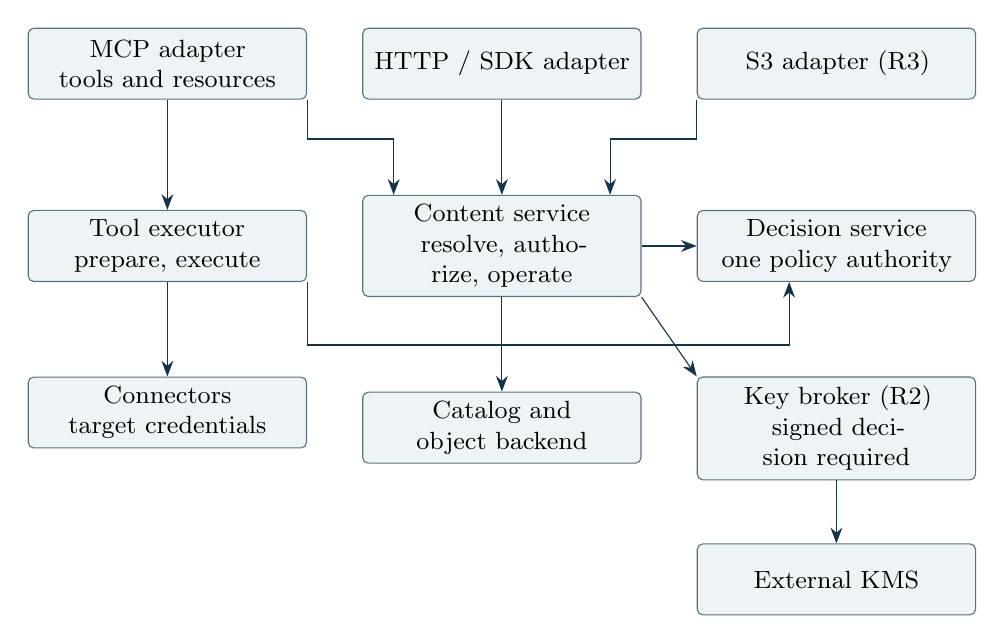
\begin{tikzpicture}[box/.style={draw=ink!70,rounded corners=2pt,fill=pale,align=center,minimum height=9mm,text width=33mm,font=\small},arr/.style={-{Stealth[length=2mm]},ink}]
\node[box] (mcp) {MCP adapter\\tools and resources};
\node[box,right=7mm of mcp] (http) {HTTP / SDK adapter};
\node[box,right=7mm of http] (s3) {S3 adapter (R3)};
\node[box,below=14mm of mcp] (exec) {Tool executor\\prepare, execute};
\node[box,right=7mm of exec] (content) {Content service\\resolve, authorize, operate};
\node[box,right=7mm of content] (dec) {Decision service\\one policy authority};
\node[box,below=12mm of exec] (conn) {Connectors\\target credentials};
\node[box,below=12mm of content] (store) {Catalog and\\object backend};
\node[box,below=12mm of dec] (broker) {Key broker (R2)\\signed decision required};
\node[box,below=8mm of broker] (kms) {External KMS};
\draw[arr] (mcp) -- (exec);
\draw[arr] (mcp.south east) -- ++(0,-5mm) -| ([xshift=4mm]content.north west);
\draw[arr] (http) -- (content);
\draw[arr] (s3.south west) -- ++(0,-5mm) -| ([xshift=-4mm]content.north east);
\draw[arr] (content) -- (dec);
\draw[arr] (exec.south east) |- ++(0,-8mm) -| ([xshift=-6mm]dec.south);
\draw[arr] (content) -- (store);
\draw[arr] (exec) -- (conn);
\draw[arr] (content.south east) -- (broker.north west);
\draw[arr] (broker) -- (kms);
\end{tikzpicture}
\caption[Architecture overview]{One access-controlled system, several protocol interfaces. Process isolation and replication do not create different resources or permission systems.}
\end{figure}
\begin{longtable}{@{}P{0.11\textwidth}P{0.50\textwidth}P{0.10\textwidth}@{}}
\toprule Role (\code{fga serve --role=}) & Hosts & Phase\\\midrule\endhead
\code{decision} & Decide/DecideBatch, context resolver, snapshot activation, decision-signing key & R1-A\\
\code{control} & Control API, catalog administration, approvals, reservations, policy releases & R1-A\\
\code{tools} & Tool executor, connectors, MCP adapter & R1-B\\
\code{storage} & Content service, HTTP handlers, external-backend adapter (S3 handlers in R3) & R1-C\\
\code{keys} & Key broker, KMS client, recipient registry & R2\\
\code{blob} & Replicated blob service and repair (when the custom backend is selected) & R3\\
\bottomrule
\end{longtable}
Roles are deployment and security boundaries of one product, not separate permission domains. The decision service is the only evaluator; no adapter, executor or broker evaluates policy.

\subsection{Phase 0 decisions}\label{sec:decisions}
These decisions are open. Each has a default so that work can be planned, but the default is not a decision until the owner records it. Work gated by a decision does not start before it is closed.
\begin{longtable}{@{}P{0.06\textwidth}P{0.22\textwidth}P{0.46\textwidth}P{0.12\textwidth}@{}}
\toprule ID & Decision & Options (default first) & Gates\\\midrule\endhead
D-01 & Policy evaluator & Decided: our own evaluator for our own policy format (Section~\ref{sec:policyformat}). Upstream engines are studied for ideas only (D-03). & R1-A\\
D-02 & Object storage & Decided: our own object storage. R1 is a single-node store on local disk with the catalog in PostgreSQL; replication comes later and the S3-compatible API in R3. Everything runs locally for now. & R1-C\\
D-03 & Upstream study and license record & Decided in principle: MinIO and Cerbos are studied for ideas only, and no upstream code is copied, translated or reproduced (\rr{SRC-001}). The license record is completed before first distribution (\rr{SRC-004}). & P0\\
D-04 & Identity providers and workload identity & Supported OIDC providers; how workload certificates are issued, rotated and bound to roles (\rr{TRU-002}). & R1-A\\
D-05 & PostgreSQL HA and failure domains & HA controller, quorum-commit configuration and the physical failure-domain topology (\rr{AVL-001}). & R1-C\\
D-06 & Label order and label sources & Per-tenant classification order; who may label and which classifier workloads are trusted (\rr{LAB-002}). & R1-C\\
D-07 & First downstream connector & The one real tool provider used to qualify the executor (\rr{SMALL-003}). & R1-B\\
D-08 & KMS and seal/unseal mechanism & Reference provider, seal mechanism and recovery custody (\rr{KEY-005}). & R2\\
D-09 & Key hierarchy & Flat per-unit wrapping is the baseline. The two-level hierarchy (KEK per document version, \rr{KEY-001}) is adopted only if the sizing measurements (\rr{SIZ-001}) show a benefit that outweighs its wider compromise impact. & R2\\
D-10 & Limits and S3 client set & Tenant workload limits, object-size limits, and the conformance client list (\rr{S3P-005}). & R3\\
D-11 & Name and distribution license & Product name, license of original code, license compatibility of dependencies (\rr{SRC-004}). & first release\\
\bottomrule
\end{longtable}

\subsection{Conventions}
Requirements have the form \textbf{[ID]} statement \reqtag{phase}{tests}. Each states one obligation. The phase is one of P0, R1-A, R1-B, R1-C, R2, R3. The tests are identifiers from Section~\ref{sec:testmatrix}; \code{REV} means a release review item and \code{LINT} means the specification check. A superscript \textsuperscript{\color{accent}\tiny NEW} marks a requirement that is new in version 2.0; Appendix~\ref{app:mapping} maps every version 1.3 requirement to its successors.

\must, \mustnot\ and \should\ carry their usual normative meaning. Limits and numbers marked ``initial'' or ``target'' are proposals to be qualified, not measured properties. Sizes use KiB = 1024 bytes. Money uses integer minor units with an explicit currency (\rr{DAT-005}).

Test vectors in \texttt{vectors/} and Appendix~\ref{app:vectors} define concrete inputs and expected outcomes. They are part of the specification (\rr{TEST-003}).

\section{Decision core}\label{sec:decision}
Part~1 defines who is acting, on what, how a decision is made, how it is bound to an operation, and how the authority state is released, stored, audited and kept available. It does not depend on storage, documents or encryption.

\subsection{Identity and trusted context}
\req{ID-001}{R1-A}{T-03}{Identity comes only from verified OIDC or OAuth tokens, workload certificates, signed S3 credentials, or another explicitly registered authentication provider. Issuer, audience, signature, expiry and intended use are validated.}
\req{ID-002}{R1-A}{T-03}{The platform \mustnot\ accept an agent- or caller-supplied role, tenant, delegation, device state or user identifier as authority.}
\req{ID-003}{R1-A}{T-03}{Adapters submit references and operation facts. The context resolver loads roles, ownership, labels, grants, session limits and approved external signals from authoritative state.}
\req{ID-004}{R1-A}{T-03}{Every trusted context field records its source, observation time, maximum age and revision where available. A missing or stale mandatory envelope fact (verified identity, tenant binding, delegation, version binding) rejects the operation.}
\req{ID-005}{R1-A}{T-03}{External lookups complete before evaluation under a bounded deadline. Policy expressions \mustnot\ fetch data or invoke tools.}
\req{ID-006}{R1-A}{T-03}{Managed-device and recent-authentication facts are usable by policy only when a trusted provider supplies them. A declared purpose may be recorded and constrained but \mustnot\ be inferred as intent. Network origin is trusted only through configured proxies that strip and regenerate forwarding headers.}
\req{ID-007}{R1-A}{T-03}{An ID token \mustnot\ be accepted as an API access token. A JWT access token is accepted only under the resource server's explicit token profile, and opaque tokens only through the provider's supported introspection flow. One JOSE implementation serves all token and envelope signature checks.}

\subsection{Delegation}
The \term{actor} is the executing workload or user. The \term{subject} is the user or service whose authority it exercises. An agent acting for a person carries both; neither inherits the other's full rights.
\req{DLG-001}{R1-A}{T-03}{A delegation record binds actor, subject, audience or executor, resource and action scope, expiry, parent delegation and an optional budget.}
\req{DLG-002}{R1-A}{T-03}{A child delegation can only narrow its parent. Delegation depth is bounded; cycles and unknown parent revisions are rejected.}
\req{DLG-003}{R1-A}{T-01, T-03}{The business-policy principal is the represented subject. Without a delegation the authenticated actor is the principal. Actor and subject role sets \mustnot\ be merged.}
\req{DLG-004}{R1-A}{T-03}{The actor's execution capability and the delegation ceiling are validated independently of business policy. Effective authority is the intersection of actor capability, delegation scope and subject permission.}
\req{DLG-005}{R1-A}{T-03, T-13}{Revocation advances a delegation generation that is checked at admission and at commit.}
\req{DLG-006}{R1-A}{T-03}{A static API key shared by several agents does not identify the user behind each call. A connector using one \mustnot\ claim user-specific enforcement without a verified delegation channel.}
\req{DLG-007}{R1-A}{T-03}{Default credentials carry no implicit administrator or cross-tenant grant. Cross-tenant access requires an explicit, reviewed sharing construct and \mustnot\ result from a missing tenant filter.}

\subsection{Resources, actions and canonical identity}
A \term{check} is one action on one resource binding. A compound operation is several checks evaluated in one batch, all of which must succeed (\rr{RES-006}).
\begin{longtable}{@{}P{0.25\textwidth}P{0.25\textwidth}P{0.31\textwidth}P{0.08\textwidth}@{}}
\toprule Resource type & Example actions & Protected facts & Phase\\\midrule\endhead
\code{agent.tool} & discover, invoke, configure & Registry identity, schema digest, connector, capability class & R1-B\\
\code{network.destination} & connect, send & Approved hostname or service identity, port, destination class, clearance & R1-B\\
\code{business.record} & read, update, approve, export & Organization, owner, workflow state, sensitive fields & R1-B\\
\code{document.version} & read-units, raw-read, discover & Canonical document and version, immutable manifest, full-content coverage & R1-C\\
\code{document.text_unit} & read, use-in-model, export-key & Canonical unit and object version, label, lineage & R1-C\\
\code{document.derived} & deliver, declassify, relabel & Lineage, effective label, intended recipient & R1-C\\
\code{text.entry} & read, use-in-model, update & Versioned text unit, parent collection & R1-C\\
\code{storage.object} & read, stat, discover, new-version, delete & Tenant, owner, project, label, immutable version, publication state & R1-C\\
\code{storage.bucket} & create-object, list, manage & Retention and encryption requirements, namespace restrictions & R1-C\\
\code{ai.model} & submit, configure & Approved provider and model, endpoint, credential binding & R1-C\\
\code{platform.policy} & propose, test, approve, activate & Bundle digest, reviewer, tenant scope, activation generation & R1-A\\
\code{crypto.recipient} & enroll, activate, receive-key, revoke & Principal or workload binding, immutable key fingerprint, purpose, status & R2\\
\code{crypto.envelope} & create, release, rewrap, retire & Object, tenant and version binding, wrapping-key reference, status & R2\\
\code{storage.replica} & repair, inspect, retire & Blob identity, node incarnation, placement generation & R3\\
\bottomrule
\end{longtable}
\req{RES-001}{R1-A}{T-01, T-06}{Every protected operation maps to one or more (resource, action) checks from the registry. An operation with no registered mapping fails closed.}
\req{RES-002}{R1-A}{T-06}{A canonical resource registry maps S3 bucket, key and version, MCP URI and tool selectors to the same tenant-scoped resource UUID, immutable content version, policy kind, version and scope, and trusted attributes. Role membership and principal context resolve through one identity pipeline.}
\req{RES-003}{R1-A}{T-01, T-06}{Content reading uses the canonical action \code{read}. Legacy route names such as \code{storage.object.read} are aliases, not competing policies. A caller \mustnot\ obtain a less restrictive policy kind or scope by changing protocol.}
\req{RES-004}{R1-A}{T-06}{Alias resolution happens once under a declared catalog snapshot and is bound to the operation. The resource generation is revalidated before admission and publication. ``Latest'' \mustnot\ be resolved again after authorization.}
\req{RES-005}{R1-A}{T-06}{A rename changes a namespace alias, not the resource's permission identity. An edit creates a new immutable version.}
\req{RES-006}{R1-A}{T-06}{A compound operation requires a separate allowed check for every resource and action it actually needs. One allow \mustnot\ authorize an unrelated effect, and \code{tool.invoke} alone \mustnot\ authorize reading the tool's source object or sending to its destination.}
\req{RES-007}{R1-A}{T-01, T-06}{A channel difference affects a decision only through an explicitly declared, trusted context attribute that the policy deliberately uses. Authentication or unsupported-protocol failures stay separate restrictions and \mustnot\ turn a business denial into an allow.}
\req{RES-008}{R1-A}{T-06}{Parent-resource checks configured for a content family apply identically through every transport as explicit compound checks, not as a hidden change to scope inheritance.}

\subsection{Policy evaluation}\label{sec:policy}
\subsubsection{Evaluator contract}
The decision service calls the business evaluator through a narrow contract so that the engine behind it (decision D-01) can be native or upstream.
\begin{lstlisting}
// Logical contract. Pure: no I/O, no ambient state, time passed in.
EvaluatorRequest {
  snapshot_digest,
  policy_set: BUSINESS | CEILING,
  principal: {id, roles, attrs},
  resource:  {kind, id, version, scope, attrs},
  actions:   [string],
  aux:       {envelope facts mapped as documented attributes},
  now
}
EvaluatorResult {
  per_action: [{action, effect, outputs, metadata, diagnostics}],
  errors:     [{action, kind}]          // strict mode: affected action is DENY
}
\end{lstlisting}
\req{POL-001}{R1-A}{T-01}{Business policy evaluation sits behind the evaluator contract. The conformance corpus (\rr{TEST-003}) applies to any engine that implements the contract.}
\req{POL-002}{R1-A}{T-01, T-02}{The evaluator implements the project's own policy format and evaluation rules of Section~\ref{sec:policyformat}. A document or construct that the format does not define is rejected at bundle validation and \mustnot\ be silently ignored.}
\req{POL-003}{R1-A}{T-01}{Evaluation proceeds in this order: (1) authenticate and validate the execution envelope; (1b) evaluate the ceiling set for every check, as an always-run gate that does not depend on the business result; (2) normalize resource, action and principal input and resolve the scope chain; (3) evaluate the business set by the rules of Section~\ref{sec:policyformat}, in which a matching deny always overrides an allow; (4) apply the business result unchanged to that check and combine it with the ceiling result so that a ceiling \code{DENY} always wins; (5) fulfil platform prerequisites and obligations. Platform steps add rejections only and \mustnot\ turn a business denial into an allow.}
\req{POL-004}{R1-A}{T-01}{The response records the business decision and any platform rejection reason separately. A protocol or authentication failure \mustnot\ be reported as a policy-combination rule, and no adapter implements alternate granting logic.}
\req{POL-005}{R1-A}{T-02}{Evaluation is strict. An error in the condition of any candidate rule for a requested action yields \code{DENY} for that action, or an objection in the ceiling set. The format has no lenient mode, so no configuration can select one.}
\req{POL-006}{R1-A}{T-02}{A missing business attribute is handled by the production profile and \mustnot\ fall through to an allow. Trusted-envelope facts never depend on business-schema settings: invalid credentials, wrong tenant or resource binding, unavailable authority, malformed transport, process faults and exhausted limits always reject.}
\req{POL-007}{R1-A}{T-01, T-02}{Platform ceilings are a separate, deny-only ceiling set in the signed bundle. Every check is also evaluated against the ceiling set through the evaluator contract (\code{policy_set: CEILING}) before and independently of the business evaluation, and a ceiling \code{DENY} or a ceiling evaluation error denies the check whatever any principal, role, derived-role or scope result says. Bundle validation rejects a ceiling set that contains a principal policy, an allow rule or a scope override.}
\req{POL-008}{R1-A}{T-01}{Time is captured freshly for each request or batch and never frozen at bundle preparation. Admission and commit checks use current server time.}
\req{POL-009}{R1-A}{T-02}{Policy expressions cannot fetch network data, read files, execute scripts or acquire credentials. Compilation, input size, evaluation cost, memory and concurrency are bounded independently of business-policy options.}
\req{POL-010}{R1-A}{T-01}{A snapshot is prepared once per immutable bundle. It contains the validated policy graph, schemas, checked executable expressions, configuration and dispatch indexes keyed by static resource, action, version and scope facts. The index \mustnot\ omit a rule because another path looks permissive. A compiled expression is shared only when the complete environment identity (types, function signatures, schema digests, library and options versions, cost model, evaluator-semantics version) matches.}
\req{POL-011}{R1-A}{T-01}{Policy outputs are data. A mapping from selected output fields to platform obligations is allowed only when explicitly configured, versioned and validated. No mandatory proprietary policy field is introduced for approvals or storage behavior.}
\reqn{POL-012}{R1-A}{T-01}{The conformance corpus of policy-evaluation vectors is part of this specification and runs against the engine in CI. No upstream engine is used as a reference or oracle (D-01).}
\req{POL-013}{R1-A}{T-02}{YAML authoring is converted offline into the same strict typed representation as JSON. Ambiguous or unsafe constructs are rejected, and evaluation never runs a YAML parser.}
\reqn{POL-014}{R1-A}{T-01}{Scopes form a dot-separated chain from the request's scope to the root. Rules from every scope on the chain are combined by the same deny-overrides rule, so a child scope can add allows but cannot lift a deny from a parent scope or from the root.}

\subsubsection{Policy format}\label{sec:policyformat}
The policy format is the project's own (D-01). A document holds rules for one resource type in one scope and one policy set:
\begin{lstlisting}
{
  "format": "fga.policy/v1",
  "set": "business",
  "resource": "document.text_unit",
  "scope": "acme",
  "rules": [
    {"id": "reviewers-read-own-projects",
     "effect": "allow",
     "actions": ["read"],
     "roles": ["reviewer"],
     "when": "resource.attributes.project_id in principal.attributes.project_ids"}
  ]
}
\end{lstlisting}
The ceiling set uses the same document shape with \code{"set": "ceiling"} and deny rules only, for example a rule that denies \code{read} for any role \code{when} the unit is not LIVE.

For one principal, resource and action, the engine:
\begin{enumerate}
\item collects the candidate rules of the requested set for the resource type from the request's scope and each ancestor up to the root;
\item treats a rule as matching when it lists the action (or \code{*}), the principal holds one of its roles (or \code{*}), and its condition is true or absent;
\item for the business set, returns \code{DENY} if any matching rule denies, otherwise \code{ALLOW} if any matching rule allows, otherwise \code{DENY};
\item for the ceiling set, reports an objection if any matching rule denies, and no objection otherwise;
\item denies (or objects) when the condition of any candidate rule fails to evaluate.
\end{enumerate}
An allow rule in the business set may list prerequisites in \code{requires} (\code{approval}, \code{reservation}). An allowed check carries the union of the prerequisites of every matching allow rule, and the decision is \code{NEEDS_APPROVAL} or \code{NEEDS_RESERVATION} until the prerequisite is satisfied through the control plane (\rr{APR-001}, \rr{APR-007}).

Conditions are CEL expressions over \code{principal} (\code{id}, \code{roles}, \code{attributes}), \code{resource} (\code{type}, \code{id}, \code{scope}, \code{attributes}) and \code{request} (\code{now}). They are compiled once per bundle and run under a cost limit. Because a deny always overrides an allow, holding an extra role cannot undo a deny, and no business rule can bypass a ceiling. Principal-specific policies, derived roles, shared variables and outputs are not part of version 1; they can be added later without changing the meaning of existing policies.

\subsection{Decision API}\label{sec:decisionapi}
\begin{lstlisting}
DecideBatch request {
  request_id, tenant_id, adapter_id, operation_id,
  actor:      {id, type, identity_revision},
  subject:    {id, type, identity_revision},
  delegation: {id, revision},
  session:    {id, binding_revision, context_key,
               mark_revision, label_order_generation},
  checks:     [{check_id, action,
                resource: {type, id, version, generation, metadata_revision}}],
  operation_digest, required_policy_epoch, deadline
}
DecisionResponse {
  outcome: ALLOW | DENY | NEEDS_APPROVAL | NEEDS_RESERVATION | ERROR,
  reason_code, decision_id,
  policy_results: [{check_id, principal_id, resource_id, action,
                    business_effect | NOT_EVALUATED, ceiling_effect,
                    policy_outputs,
                    policy_metadata, diagnostics}],
  bundle_digest, policy_epoch, evaluator_version,
  actor_id, subject_id, delegation_revision,
  operation_digest, resource_bindings_digest, context_revisions,
  evaluated_at, valid_until,
  obligations: [{type, version, parameters_or_ref, parameters_digest}],
  session_mark_revision_after,
  signature                       // detached JWS, see DEC-008
}
\end{lstlisting}
\code{Decide} is a batch of one. A platform-gate rejection returns \code{DENY} with a platform reason code and \code{NOT_EVALUATED} business effects. \code{ERROR} means the service could not decide (timeout, unavailable authority, resource limit).
\req{DEC-001}{R1-A}{T-01}{The decision API is exposed as versioned gRPC for internal services and an authenticated JSON facade for SDKs. The caller \mustnot\ choose an action mapping different from the registered operation.}
\req{DEC-002}{R1-A}{T-01}{The enforcement point acts only on an explicit, complete \code{ALLOW} bound to its exact operation. \code{DENY}, \code{NEEDS_APPROVAL}, \code{NEEDS_RESERVATION}, \code{ERROR}, transport errors, malformed data, unknown required obligations and missing results all stop execution. A prerequisite outcome is satisfied through the control plane, after which a new \code{ALLOW} whose context revisions include the approval or reservation is required.}
\req{DEC-003}{R1-A}{T-01}{Each response carries the per-check business and ceiling effects, outputs, metadata, redacted diagnostics, bundle digest, policy epoch, evaluator version, identity and delegation revisions, operation and resource-bindings digests, validity and obligations. A platform gate that stops evaluation is reported with an explicit not-evaluated marker and \mustnot\ authorize execution.}
\req{DEC-004}{R1-A}{T-01}{A batch captures one policy snapshot and one authority envelope. Items have unique identifiers and exact resource, action and revision bindings. A missing, duplicated or misbound result \mustnot\ authorize its operation, and a failed item \mustnot\ grant its peers. A batch is an evaluation optimization, not a transaction over writes or external effects.}
\req{DEC-005}{R1-A}{T-13}{\code{valid_until} is bounded by the earliest of identity or session expiry, delegation expiry, approval or grant expiry, context freshness limit, request deadline and a conservative decision-age limit. A decision is not a general bearer permission.}
\req{DEC-006}{R1-A}{T-13}{At read admission and immediately before a mutation's irreversible or egress checkpoint, the executor rechecks expiry and every authority-bearing revision recorded with the decision: resource generation; metadata revision; access and label revisions of the parent and of each selected unit; delegation and identity revisions; context mark revision and label-order generation; and the required policy epoch. A mismatch requires a new decision or rejection. The executor uses the same canonical operation that was evaluated.}
\req{DEC-007}{R1-A}{T-03}{Identity and capability checks are enforced at the decision API itself. mTLS workload identity or an equivalent bound credential identifies the adapter, and an ordinary user cannot submit fabricated verified context.}
\reqn{DEC-008}{R1-A}{T-03}{The decision service signs each \code{ALLOW} record with a registered decision-signing key, used for no other purpose, whenever the decision will be used across a process or role boundary or retained. The signed bytes are one canonical serialization (strict JSON with no unknown or duplicate fields, signed exactly as transmitted) containing: decision ID; audience (deployment, role and service); tenant; actor, subject, delegation and context identity with their revisions; operation digest; every check with its resource binding and effect; bundle digest and policy epoch; access, label and context-mark revisions and the label-order generation; and issue time and \code{valid_until}. A verifier checks signature, audience, validity and the replay rule, and still performs the fresh revision checks of \rr{DEC-006}: a signature does not replace them. A role \mustnot\ accept a decision whose audience is another role. A signed decision proves that the sole authority evaluated the request it describes; it is not proof that the user's intent or the request's context was validly established.}
\req{DEC-009}{R1-A}{T-22}{Initial qualification limits are a 250 ms single-decision budget, 64 KiB of context, 50 resources per batch, 8 KiB of expression text, bounded AST depth, 10,000 expression cost units per condition and a total request budget. These are proposed limits, not measured guarantees; independent input, compilation, allocation, concurrency and cancellation limits are mandatory, and cancellation reaches both queued and running evaluation.}
\req{DEC-010}{R1-A}{T-01}{Error diagnostics distinguish a policy denial from a service failure without exposing protected details to unauthorized clients.}
\reqn{DEC-011}{R1-A}{T-03}{Consumption of a single-use signed decision (mutation and key release) is an atomic, durably acknowledged compare-and-set in the catalog, shared by every replica of the verifying role and recorded before the effect begins. A replica that cannot reach the consumption store refuses the decision.}
\reqn{DEC-012}{R1-A}{T-03}{Decision-signing keys are distinct from workload, issuer and encryption keys. Key identifiers reach verifiers through the control plane, rotation uses an overlap window no shorter than the longest \code{valid_until} plus clock skew, and a compromised signing key is revoked by a revision that verifiers must observe before accepting further decisions. Rotation and revocation are qualified under T-03.}

\subsection{Policy releases and readiness}
\req{REL-001}{R1-A}{T-14}{A policy release is an immutable, signed bundle whose manifest includes schema and evaluator versions, source hashes, the business set, the ceiling set, the label order and its generation, resource schemas, operation registry, pure-function allowlist, expression-library version and cost model, test evidence, target audience and digest. Each instance verifies, parses, compiles, validates and checks a candidate into an immutable in-memory snapshot before atomically replacing its active pointer. A failed activation preserves the prior valid state and does not acknowledge the candidate.}
\req{REL-002}{R1-A}{T-14}{Activation records the states RECEIVED, VERIFIED, PREPARED, READY, ACTIVE or REJECTED with digest, environment version, preparation error and timestamps. Every decision uses exactly one snapshot, and preparation and old-snapshot coexistence are resource-bounded.}
\req{REL-003}{R1-A}{T-13, T-14}{A node that cannot establish the authoritative required epoch \mustnot\ authorize new operations. The last valid snapshot is kept only while it satisfies that epoch. Offline authorization is not an availability fallback.}
\req{REL-004}{R1-A}{T-14}{The control plane stages a candidate pool, verifies sentinel allow and deny cases, records ready instances by digest, advances the durable tenant-required epoch, and routes only to compatible instances. A restrictive activation may stop admissions and drain bounded mutation leases. A rollback is a new reviewed release with a higher epoch, because silently reverting may restore revoked access.}
\reqn{REL-005}{R1-A}{T-14}{Before activation the candidate is run over the conformance corpus and the tenant's sentinel cases, and the change in effect against the active release is reported to the reviewer, who must acknowledge it. The report covers the corpus and sentinels only; it does not enumerate every principal.}
\req{REL-006}{R1-A}{T-14, T-19}{Liveness reports process progress and does not restart a healthy process because PostgreSQL, KMS or a peer is unavailable. Readiness is role- and capability-specific (policy digest and epoch, catalog authority, workload credential validity, required crypto and connector dependencies). Probes return redacted aggregate state, are rate-limited, and do not create a KMS key. A readiness result is never a grant; requests perform their own admission checks.}

\subsection{State and catalog}
PostgreSQL holds authoritative identities, grants, resource bindings, revisions, approvals, reservations and audit-outbox records.
\begin{longtable}{@{}P{0.20\textwidth}P{0.62\textwidth}P{0.08\textwidth}@{}}
\toprule Entity & Minimum authoritative fields & Phase\\\midrule\endhead
Principal, delegation & Stable IDs; tenant; actor and subject bindings; credential class; roles; limits; expiry; revocation and identity revisions & R1-A\\
Resource & UUID; type; tenant; protected attributes; metadata revision; resource generation; lifecycle state & R1-A\\
Policy release & Canonical manifest digest; schema, configuration, evaluator and expression-library versions; tests; publisher signature; activation epoch & R1-A\\
Audit outbox & Unique event ID; decision and operation IDs; redacted bindings; outcome; delivery status & R1-A\\
Tool registry & Stable tool ID; schema digest; connector version; operation mapper; allowed destinations; required capabilities; credential binding & R1-B\\
Invocation & Tenant and idempotency unique key; argument digest; state; dispatch attempt and fencing token; downstream receipt; reconciliation status & R1-B\\
Approval & Exact operation digest; approver; subject and actor; resource revisions; expiry; allowed uses; consumption state & R1-B\\
Reservation & Budget or grant ID; minor-unit amount or use count; invocation ID; status; lease; reconciliation state & R1-B\\
Object, version & Bucket and exact key; stable object UUID; current committed version; content generation; immutable blob ID; length and checksums & R1-C\\
Document manifest, text unit & Document and version UUIDs; ordered unit IDs; manifest digest; extraction and normalization version; unit order; labels; access revision; provenance & R1-C\\
Upload intent & Operation and idempotency IDs; principal and delegation; expected generation and current version; intended labels; staged blob; state; expiry & R1-C\\
Context mark & Context key (runtime context ID, else delegation ID); bound actor, subject and delegation; label-order generation; highest effective label; mark revision & R1-C\\
Recipient key, key envelope & Tenant; principal or workload; immutable key ID and fingerprint; purpose and suite; activation and revocation revision; wrapped keyset; generation; status & R2\\
Maintenance job & Kind; tenant and blob scope; expected placement generation; idempotency key; lease and fence; progress; initiating actor & R3\\
\bottomrule
\end{longtable}
\req{DAT-001}{R1-A}{T-01}{All authoritative lookups include tenant scope. Tenant-consistent references are enforced with database constraints or equivalent transaction checks. Tenant isolation \mustnot\ depend on policy authors writing a tenant condition.}
\req{DAT-002}{R1-A}{T-03}{Protected fields change only through explicit authorized control operations with expected revisions. Raw S3 tags, tool arguments and external payloads \mustnot\ become trusted ownership or classification records.}
\req{DAT-003}{R1-A}{T-06, T-13}{Resource metadata revision and content or resource generation are distinct. Every logical publication, deletion or target-state mutation increments the generation, and approval and execution comparisons include state changes even when access labels have not changed.}
\req{DAT-004}{R1-A}{T-13, T-14}{Permission-critical facts use authoritative consistent reads. The first release has no allow-result cache. A cache, if added, requires a maximum age, revision-aware keys and explicit invalidation. A decision uses one immutable policy snapshot and one declared context snapshot. Search indexes and storage notifications are discovery aids, not access authority.}
\req{DAT-005}{R1-B}{T-05}{Money uses integer minor units with an explicit currency. Binary floating point \mustnot\ be used for permission thresholds or budget consumption.}

\subsection{Audit}
\req{AUD-001}{R1-A}{T-15}{Decisions and actual outcomes are logged separately and joined by decision, operation and invocation IDs. Records include actor, subject, tenant, action, resource, version and generation, relevant context provenance, policy digest and epoch, reason, latency and redacted obligations. External tools record dispatch and receipt or reconciliation evidence.}
\req{AUD-002}{R1-A}{T-15}{Attempt, decision, key release, durable mutation, approval consumption and external delivery are distinct events. Mandatory records are appended transactionally to an outbox and \mustnot\ silently disappear when the exporter is disabled or a queue is full; capacity alarms and declared admission limits act before required evidence can no longer be recorded. Operational logs and optional notifications are not a substitute for the outbox.}
\req{AUD-003}{R1-A}{T-19}{Audit delivery is idempotent with explicit retention and access policies. Sensitive labels and arguments are minimized or protected, lag, loss, stale policy nodes, failed context resolution and revocation latency are monitored, and metrics \mustnot\ create a cross-tenant information channel.}
\req{AUD-004}{R1-A}{REV}{A key-release audit record proves that a key was issued, not that a user opened plaintext or complied with a purpose restriction. Documentation \mustnot\ present it as proof of use.}

\subsection{Administration}
\req{ADM-001}{R1-A}{T-20}{Policy authors, reviewers, activators, key administrators, storage operators and data users are separate roles. A policy administrator is not automatically a data reader, and sensitive policy or key changes use the approval and reservation model where configured.}
\req{ADM-002}{R1-A}{T-20}{An ordinary API request \mustnot\ disable the authorizer, change trusted issuers, relax workload audience checks, replace a key provider or grant itself policy-administrator authority. Those changes use explicit administrative actions and reviewed control transactions.}
\req{ADM-003}{R1-A}{REV}{Bootstrap and recovery authority sits outside ordinary agent paths, with controlled local or separately authenticated recovery and a durable incident audit. Recovery procedures \mustnot\ claim to defend against a host operator who can replace the running software.}

\subsection{Availability of authority state}\label{sec:availability}
This section covers the decision, control and catalog services. Blob replication is in Part~5.
\begin{longtable}{@{}P{0.20\textwidth}P{0.40\textwidth}P{0.30\textwidth}@{}}
\toprule Layer & Initial production topology & Failure contract\\\midrule\endhead
Gateways, decision, tools & At least 3 stateless replicas across 3 failure domains, required bundle digest on each & Load balancer removes unready replicas; stale or unavailable authority never becomes allow\\
Tool executors & At least 3 workers sharing durable invocation state & Leases and fencing plus downstream idempotency; no blind redispatch after timeout\\
Catalog PostgreSQL & Primary plus 2 standbys; commit durable on the primary and at least one synchronized remote standby (quorum commit) & HA coordinator promotes only a safe candidate and fences the old primary; no silent asynchronous downgrade\\
\bottomrule
\end{longtable}
\req{AVL-001}{R1-C}{T-15, T-16}{Production runs the topology above. Single-node operation is a development profile and is rejected by production configuration.}
\req{AVL-002}{R1-C}{T-16}{Authorization-critical reads use the primary or a standby proven sufficiently fresh by a log-position check. An arbitrarily lagging standby \mustnot\ restore revoked grants.}
\req{AVL-003}{R1-C}{T-16}{PostgreSQL runs with \code{fsync=on}, \code{full_page_writes=on}, \code{synchronous_commit=on} or stronger, and a non-empty synchronous standby set; \code{remote_write} alone is insufficient against an operating-system crash. With Patroni, strict synchronous mode is enabled. Failover uses a managed HA service or established controller with quorum coordination and old-primary fencing, and promoting an unqualified stale replica voids the zero-loss objective.}
\req{AVL-004}{R1-C}{T-16}{A timeout or cancellation while awaiting a synchronous commit is an unknown outcome, and a lookup by operation ID on the primary is not evidence of durability: after a cancelled wait the transaction can be visible on the primary without having been replicated. Before returning durable success, dispatching an external effect or releasing a key, the platform obtains proof that the required synchronous standbys have flushed WAL at or beyond the transaction's commit position on the current fenced timeline, either from an acknowledged synchronous commit ordered after it or from the replication flush position. Until then the outcome stays unknown.}
\req{AVL-005}{R1-C}{T-15, T-18}{The design target is zero loss of acknowledged operations under the loss of one failure domain in a crash-fault model, conditional on synchronous database acknowledgement, correct fencing and available key state; it is not a guarantee against simultaneous multi-domain loss, Byzantine replicas, malicious deletion or untested hardware. Recovery of the target service within five minutes is an acceptance objective, not a benchmark. Encrypted, access-separated backups of the catalog, policy bundles and (from R2) key envelopes and KMS recovery state are restored together in tests, and replication is not a substitute for backups.}
\req{AVL-006}{R1-C}{T-22}{Tenant-aware admission limits cover requests, bytes, active streams, expression cost, scan candidates, reservations, tool concurrency and KMS operations. Overload uses backpressure and bounded queues rather than unbounded goroutines, and retries use jitter and budgets. Circuit breakers reject rather than grant.}
\req{AVL-007}{R1-C}{T-22}{The first metadata authority is one PostgreSQL primary with HA. When measured write capacity is exceeded, tenants are sharded across independent catalog groups with an explicit tenant-to-shard registry and migration fencing, and cross-shard grants and budgets are not treated as local atomic operations. The first region is active for each tenant; multi-region active-active authorization requires a later consistency design.}

\section{Enforcement points}\label{sec:enforcement}
Part~2 defines how a decision is bound to a real operation: the adapter contract, the evidence that crosses each internal boundary, the tool executor, approvals and reservations, unknown outcomes, data-flow limits, and the MCP transport. Content-specific MCP operations are in Part~3.

\subsection{Adapter contract}
\begin{lstlisting}
// Logical design; generated DTOs are defined by the versioned API.
type EnforcementAdapter interface {
    Prepare(ctx context.Context, request AdapterRequest) (OperationPlan, error)
    Execute(ctx context.Context, plan OperationPlan, grant Grant) (Outcome, error)
}

type OperationPlan struct {
    ID              string
    RegistryVersion string
    RequiredChecks  []Check
    ArgumentsDigest string
    ResourceBindings []ResourceBinding
    IdempotencyKey  string
}
\end{lstlisting}
\req{ENF-001}{R1-B}{T-04}{Every adapter implements \code{Prepare} and \code{Execute}. \code{Prepare} resolves targets and validates arguments without performing the protected side effect. \code{Execute} verifies the grant, carries out the required obligations and dispatches only the prepared plan.}
\req{ENF-002}{R1-B}{T-04}{An adapter request is a validated typed protocol or domain variant. It \mustnot\ be an unrestricted \code{any} or an arbitrary attribute map, and each concrete adapter accepts only its declared request kind.}
\req{ENF-003}{R1-B}{T-01, T-04}{An adapter translates authentication evidence, selectors, operation parameters and response framing. It \mustnot\ fork business grants, duplicate policy combination, invent its own context format, turn an unknown policy result into a local allow, or perform a permissive check and then bypass the shared service.}
\req{ENF-004}{R1-B}{T-04}{Where target resolution is itself sensitive, it requires a separate discovery or stat action.}
\req{ENF-005}{R1-B}{T-04}{Every adapter declares its discovery, read, mutation, output-transformation, batching, streaming and obligation capabilities. An unknown capability fails closed. Public API clients receive redacted errors while internal audit retains diagnostic detail, and the resource-to-action mapping is versioned with policy and schema releases.}
\req{ENF-006}{R1-C}{T-04}{Database row or column filtering, filesystem mounts, message consumption and job scheduling are extension points that need real enforcement at their own access boundary. The first release does not compile expressions into SQL; a later optimizer must translate a declared subset, prove equivalence against per-resource decisions and never drop an unsupported predicate. A database adapter exposes a field only if it actually builds a restricted query or response.}

\subsection{Trust propagation}\label{sec:trust}
Authentication at an ingress is insufficient if a downstream service can be reached another way. Each internal call carries the evidence in Table~\ref{tab:hops}, and the receiver rejects a call that lacks it.
\begin{longtable}{@{}P{0.06\textwidth}P{0.20\textwidth}P{0.46\textwidth}P{0.10\textwidth}@{}}
\caption{Evidence that crosses each boundary}\label{tab:hops}\\
\toprule TB & Hop & Evidence the receiver verifies & Phase\\\midrule\endfirsthead
\toprule TB & Hop & Evidence the receiver verifies & Phase\\\midrule\endhead
TB1 & Client \arrowto\ adapter & Token or credential for this audience (\rr{ID-001}); session bound to actor, subject and delegation (\rr{MCP-007}) & R1\\
TB2 & Adapter \arrowto\ decision & Workload certificate bound to the adapter role (\rr{DEC-007}); references, not asserted facts (\rr{ID-003}) & R1-A\\
TB2 & Decision \arrowto\ adapter & Signed decision for this audience, operation and validity (\rr{DEC-008}) & R1-A\\
TB3 & MCP adapter \arrowto\ content service & Workload certificate of the \code{tools} role, plus signed decision or a delegation reference verified against authoritative state (\rr{TRU-003}) & R1-C\\
TB3 & Content service \arrowto\ broker & Workload certificate of the \code{storage} role plus a signed decision whose checks are exactly those of the matching operation mapping of Table~\ref{tab:keyops}, bound to the exact object, version, unit and recipient (\rr{TRU-005}) & R2\\
TB4 & Executor \arrowto\ connector & Target-specific restricted credential, never the model's credential (\rr{AGT-006}) & R1-B\\
TB4 & Executor \arrowto\ downstream & Idempotency key and state precondition where supported (\rr{AGT-006}, \rr{INV-005}) & R1-B\\
TB5 & Storage \arrowto\ blob backend & Verified workload binding on every call (\rr{BKD-001}) & R1-C\\
\bottomrule
\end{longtable}
\req{TRU-001}{R1-A}{T-03}{Each cross-process hop carries the evidence listed in Table~\ref{tab:hops}. A receiver that does not find it rejects the call.}
\req{TRU-002}{R1-A}{T-03, T-20}{Workload identity uses mTLS or an equivalent bound credential issued by the workload certificate authority chosen in decision D-04, bound to one role. Certificate verification is mandatory configuration, not an optional check.}
\reqn{TRU-003}{R1-A}{T-03}{The end user's authority crosses a hop only as a signed decision (\rr{DEC-008}) or as a delegation reference that the receiver verifies against authoritative state. Caller-asserted claims plus a workload identity are never sufficient.}
\reqn{TRU-004}{R1-A}{T-03}{A role accepts only signed decisions whose audience is that role, and the decision-signing key is registered separately from workload, issuer and encryption keys.}
\reqn{TRU-005}{R2}{T-11}{The broker releases key material only against a signed decision whose checks are exactly those of the matching operation mapping in Table~\ref{tab:keyops} and that is bound to the exact object, version, unit and recipient being released. The broker verifies the complete signed result, not a subset, whether or not the request also carries an mTLS identity. A compromised gateway therefore cannot obtain keys that no valid decision covers.}
\req{TRU-006}{R1-C}{T-03}{The MCP adapter calls the same content-service implementation as every other adapter and preserves the represented principal and delegation. It \mustnot\ replace the user with a broadly privileged connector account.}

\subsection{Tool executor}
The agent proposes an invocation. A trusted executor authenticates it, resolves the registered tool, validates arguments, computes the real operation plan, obtains authorization and performs the effect with credentials the model never sees.
\req{AGT-001}{R1-B}{T-04}{A registry record binds tool ID, version, schema digest, connector implementation, resource mapper, allowed destinations, required checks and supported obligations. Tool descriptions and annotations are untrusted unless supplied by the registry, and a label such as ``read-only'' does not establish behavior. A changed schema digest invalidates the registration until re-reviewed.}
\req{AGT-002}{R1-B}{T-04}{Hiding a tool from discovery improves usability but is not a security boundary. Every direct invocation is checked.}
\req{AGT-003}{R1-B}{T-04}{The executor performs these steps in order and \mustnot\ skip or reorder them. (1) Validate actor identity, represented subject, tenant, audience-bound session and delegation, and reject on-behalf-of headers supplied by the caller. (2) Resolve the tool and version and validate arguments against a strict schema, rejecting unknown fields where security depends on exact interpretation. (3) Map the request to concrete resources and actions (for example a submission, an account, a currency and amount, and a destination service), canonicalize them and compute the operation digest. (4) Evaluate every required check, resolve approval, reservation, destination restriction and other obligations before execution, and bind them to the exact plan. (5) At dispatch recheck expiry, generations, delegation and target binding, and use a target-specific restricted credential. (6) Execute once under the invocation record, and record success, denial, failure or unknown outcome.}
\req{AGT-004}{R1-B}{T-04}{No mutation between approval and dispatch may change tool version, target, resource, amount, destination or another security-relevant argument. Canonicalization is shared by authorization and execution.}
\req{AGT-005}{R1-B}{T-04}{The executor \mustnot\ validate one URL and then follow an arbitrary redirect to another destination. Address policy is resolved at connection time and credentials are bound to the registered service identity.}
\req{AGT-006}{R1-B}{T-04}{The connector uses a target-specific restricted credential, never the model's proposed credentials. State and version preconditions (ETag, version ID or transactional compare-and-swap) are passed downstream where authorization depends on target state, and a connector without that capability \mustnot\ claim state-bound mutation safety.}
\req{AGT-007}{R1-B}{T-03}{HTTP MCP tokens are validated for the gateway's audience and \mustnot\ be passed through to downstream APIs. The connector obtains its own limited downstream token; token-exchange and delegation profiles are tested rather than assumed.}
\req{AGT-008}{R1-B}{T-20}{Local stdio tools run through the trusted executor and an operating-system sandbox with bounded filesystem, process and network access. Tool servers are network-restricted so users cannot bypass the gateway with the same credentials. A remote policy service cannot intercept an unrestricted local shell or direct local file reads, and the documentation says so.}

\subsection{Approvals and reservations}
A pure policy decision can establish eligibility but cannot atomically consume a budget. Approvals, one-time grants and spending limits require stateful transactions in PostgreSQL.
\req{APR-001}{R1-B}{T-04}{A prerequisite approval or reservation is satisfied before execution. An approval binds the exact operation digest, actor and subject, target, relevant resource revisions, policy epoch, expiry and permitted uses, and a change to any material fact invalidates it.}
\req{APR-002}{R1-B}{T-05}{Approver authority and the prohibition on self-approval are checked separately. Approval consumption and reservation are atomic, and a model-generated assertion \mustnot\ stand in for the approval record.}
\req{APR-003}{R1-B}{T-05}{An approval is consumed at the documented execution checkpoint, not when it is merely displayed.}
\req{APR-004}{R1-B}{T-05}{A reservation cannot exceed its parent grant or budget under concurrency. Capacity is reserved under row-level locking or serializable transactions with unique operation and idempotency keys.}
\reqn{APR-005}{R1-B}{T-04}{The summary shown to an approver is rendered by the platform from the canonical operation plan (tool, target, amounts, destinations, resource list and highest source label). Agent- or model-supplied descriptions may be displayed only as clearly labeled unverified notes.}
\req{APR-006}{R1-B}{T-05}{Cancellation, expiry, outcome-unknown and compensation are distinct states.}
\req{APR-007}{R1-B}{T-04}{Obligations from several sources merge restrictively: field and destination sets intersect, required redactions union, and limits take the minimum. Conflicting or unsupported obligations reject, and obligations are capability-checked and enforced before their effect or disclosure.}

\subsection{Invocation state machine and unknown outcomes}
The states are PREPARED \arrowto\ RESERVED \arrowto\ DISPATCHING \arrowto\ SUCCEEDED, FAILED or UNKNOWN. A network timeout after dispatch is not proof that the external operation failed.
\req{INV-001}{R1-B}{T-05}{Invocation state transitions are recorded durably and each transition has one writer under the invocation lease.}
\req{INV-002}{R1-B}{T-05}{A unique invocation row and a transactional lease with a monotonically increasing fencing token give exactly one worker dispatch ownership. Approval consumption and budget reservation commit with the ownership transition, and in the production topology that transition passes the durability barrier of \rr{AVL-004} before the external dispatch begins.}
\req{INV-003}{R1-B}{T-05}{A replacement worker reconciles a DISPATCHING or UNKNOWN invocation and \mustnot\ redispatch it blindly.}
\req{INV-004}{R1-B}{T-05}{A retry of the same operation uses the same idempotency identity and exact argument digest. Changing arguments starts a new operation that requires new authority. Read-only calls may use a separate bounded retry policy.}
\req{INV-005}{R1-B}{T-05}{Retrying a mutation requires downstream idempotency support or target-specific reconciliation. No exactly-once promise is made across arbitrary external APIs, and tool-worker fencing cannot stop an already-running remote request unless the downstream enforces an idempotency, fencing or precondition token.}
\reqn{INV-006}{R1-B}{T-05}{An UNKNOWN invocation is resolved by connector reconciliation, or by an \code{invocation.resolve} action that records evidence and one of three outcomes: success, failure verified by evidence, or abandoned (\rr{INV-009}). The tool's maximum hold age triggers escalation and alarms (at half and at the full age) and never infers failure. For financial or destructive effects the resolver \mustnot\ be the original requester.}
\req{INV-007}{R1-B}{T-05}{A reservation for an operation with an unknown external outcome \mustnot\ be released as though no effect occurred. It remains until reconciliation or resolution commits or releases it.}
\reqn{INV-009}{R1-B}{T-05}{ABANDONED closes the workflow without establishing that the external effect did not happen. It keeps the reservation charged, keeps the approval consumed, prohibits redispatch of the operation and retains the evidence. A reservation is released only by a verified failure or by a separate \code{reservation.write-off} action, authorized to a principal other than the requester, that records the accepted risk.}
\req{INV-008}{R1-B}{T-05}{After an ambiguous failover, connectors that cannot reconcile remain UNKNOWN. The same rule applies to budget accounting and approval consumption.}

\subsection{Data flow and the context high-water mark}\label{sec:flow}
\req{FLW-001}{R1-C}{T-21}{Read permission does not constrain what a model subsequently infers, says or sends. Enforcing destination restrictions requires mediation of all relevant egress, file writes and downstream tool calls; if the model has an unrestricted independent network path, the deployment \mustnot\ claim complete output-flow enforcement.}
\req{FLW-002}{R1-C}{T-21}{A tool that reads confidential storage and sends data requires both source-read and destination-send permission, executed through one prepared plan. Raw storage and KMS credentials are not exposed to the model.}
\reqn{FLW-003}{R1-C}{T-21}{For every mediated execution context the platform records the highest effective label of any unit or derived output disclosed to it (tool results, resource reads, model context). An egress-capable call whose destination clearance is below the mark is \code{DENY}, or \code{NEEDS_APPROVAL} when a policy output says so. The mark only increases within its context.}
\reqn{FLW-004}{R1-C}{T-21}{Labels form a tenant-defined total order in the signed bundle, identified by an order generation, and the order is immutable within a generation. A unit or output with no label counts as the highest level. A mark records the generation it was computed under; when the active generation changes, a mark from an older generation is treated as the highest level unless the bundle supplies a verified monotone mapping from the old order to the new one.}
\reqn{FLW-005}{R1-C}{T-21}{The mark is conservative: it cannot tell which disclosed content influenced a call, so it over-restricts. It does not cover paths outside mediated tools, or runtimes that discard their context lifetime, and product documentation states those limits.}
\reqn{FLW-007}{R1-C}{T-21}{A mark raise is an atomic, monotonic update that is durably acknowledged before any byte of the disclosure is emitted. The decision request carries the mark revision and label-order generation, and the signed decision binds them. At egress dispatch the executor rechecks the mark revision under the invocation lease and rejects the dispatch, requiring a new decision, if the mark has risen since. Once an external call or stream is admitted and dispatched, a later raise does not retract it.}
\reqn{FLW-008}{R1-C}{T-21}{The mark belongs to a trusted execution-context lifetime. It is keyed by a context ID from a registered runtime when one is supplied, and otherwise by the delegation ID. A new MCP connection or session ID under the same key inherits the mark, and only a new key starts at the lowest level. A mark is reset early only by an explicit, audited, approval-gated \code{context.reset} action. The guarantee holds for runtimes that preserve their context lifetime (\rr{FLW-005}).}
\req{FLW-006}{R1-C}{REV}{Classification propagation and output inspection beyond the mark are separate mechanisms with explicit false-negative and false-positive limits. ``Use only for purpose X'' cannot be guaranteed by an ordinary boolean policy or by encryption alone.}

\subsection{MCP transport and surface}
\req{MCP-001}{R1-C}{T-06}{The MCP endpoint uses the official MCP Go SDK for protocol transport and JSON-RPC machinery. Project code supplies the trusted registry, policy mapping and execution boundary; a hand-written transport is not the default.}
\req{MCP-002}{R1-C}{T-06}{MCP has no independent permission rules, document store, user database or evaluator. Its handlers translate requests and responses and delegate to the shared content and decision paths.}
\req{MCP-003}{R1-C}{T-06, T-09}{Discovery and invocation are checked separately from content access. \code{tools/list} or a permit for \code{documents.read} as a tool does not authorize every document. \code{resources/read} and every content-returning tool resolve the exact resource, authorize the parent and units, and only then obtain and return permitted plaintext. A connector that cannot identify the protected content before disclosure is rejected or restricted to a fully authorized whole-resource profile, and an opaque upstream tool result is not assumed filtered.}
\req{MCP-004}{R1-C}{T-03, T-04}{Document and tool content is untrusted data, never a source of roles, permissions, trusted key locations or execution authority. Retrieved instructions cannot change the tool registry, broaden a delegation, choose a new provider endpoint or grant a follow-up tool call, and the executor checks each new effect under the same contract.}
\req{MCP-005}{R2}{T-10}{Standard MCP clients receive authorized plaintext or resource links. HPKE ciphertext is returned only to clients that explicitly support the export profile.}
\req{MCP-006}{R1-C}{T-06}{Where MCP runs in a different role process, its authenticated RPC client calls the same service implementation and preserves the represented principal and delegation.}
\reqn{MCP-007}{R1-C}{T-21}{An MCP or tool session identifier is bound to the authenticated actor, subject and delegation, and its binding revision is part of the decision request. A session identifier alone is never authority and does not by itself define the lifetime of the context mark (\rr{FLW-008}).}

\subsection{HTTP, service and future adapters}
\req{ADP-001}{R1-C}{T-06}{HTTP middleware authenticates the caller, resolves the route and resource, validates the request body and checks the exact semantic action immediately before protected work. Path parameters and request bodies are not authoritative ownership records.}

\section{Object storage, documents and fine-grained access}\label{sec:content}
Part~3 defines the storage product delivered in R1: a native object API, a canonical namespace and version catalog, durable publication, and the fine-grained access controls shared by objects, documents and text units. HTTP clients and applications can use this product with no MCP server, tool executor or model provider deployed. R1-B delivers the object service and R1-C adds document and text projections over the same objects. Every payload is stored encrypted under its bucket's mode (\rr{ENC-001}): in server mode, the default, the storage role encrypts uploads and decrypts for authorized readers under data keys released by the \code{keys} role; in client mode, clients encrypt before upload and decrypt after authorized download, and the server stores ciphertext and opaque recipient envelopes only. R1-C gives independently protected units separate keys in both modes. Part~4 defines both modes and their key ownership. Backend encryption at rest remains an additional layer. MCP is a later service client of this foundation, not its storage or authorization authority.

\subsection{Storage application service and native API}
\begin{lstlisting}
// Logical application interface; all callers retain verified identity context.
type ContentService interface {
    Read(ctx context.Context, req ReadContentRequest) (ContentPackage, error) // plaintext (server mode) or encrypted package (client mode)
    Stat(ctx context.Context, req StatContentRequest) (ContentMetadata, error)
    List(ctx context.Context, req ListContentRequest) (ContentPage, error)
    Write(ctx context.Context, req WriteContentRequest) (PublishedVersion, error)
    Delete(ctx context.Context, req DeleteContentRequest) (DeleteOutcome, error)
    Export(ctx context.Context, req ExportContentRequest) (ExportHandle, error)
}
\end{lstlisting}
\req{CNT-001}{R1-B}{T-06}{\code{internal/content} is the single application layer for content reads, stat and discovery, listing, writes, deletion, authorized envelope delivery and server-mode key release. The native HTTP API delegates to it in R1, the MCP service calls its authenticated API in R2, and S3 handlers delegate to it in R3. It resolves canonical aliases and versions and performs the business checks and mandatory guards. A client-mode read returns an encrypted package: exact ciphertext, its bound signed descriptor or authorized manifest projection, and an existing envelope for the authorized recipient under Table~\ref{tab:keyops}; the service never receives client-mode payload keys or decrypts client-mode payloads. A server-mode read returns plaintext over the authenticated connection, decrypted by the storage role with a data key released under \rr{SSE-003}.}
\req{CNT-002}{R1-B}{T-06}{Protocol adapters translate authentication evidence, selectors, operation parameters and response framing. They \mustnot\ perform a permissive content check and then bypass the shared service.}
\req{CNT-003}{R1-C}{T-06}{For a document registered with protected units, an original-file path authorizes its complete disclosure set. Parent permission or a permitted section cannot authorize a forbidden section through the encrypted original, its envelope or a server-mode original read. The original is a separate encrypted object with a separate key; delivery requires the authoritative full-content binding and every required decision. Selected unit keys never decrypt the original. Authorized-subset projection is explicit and does not silently change an ordinary object download.}
\req{CNT-004}{R1-B}{T-09}{HEAD and error responses \mustnot\ reveal existence or metadata to callers that lack stat or discovery authority.}
\req{CNT-005}{R1-B}{T-09}{A listing authorizes bucket listing, scans committed catalog candidates in stable key order, batch-checks per-object discovery, and accumulates visible entries until the page size or a bounded scan or time budget is reached. A short or empty page may carry a continuation token and the cursor must make progress. Metadata is filtered as well as names. A continuation token binds tenant, principal, identity revision, query, prefix and delimiter, policy epoch, recovery incarnation, expiry and last scanned position; its contents are encrypted and authenticated or held in opaque server state, and replay under another identity or a changed query fails. \code{CommonPrefixes} \mustnot\ expose hidden children, and delimiter support stays disabled until safe prefix discovery passes tests.}
\req{CNT-006}{R1-B}{T-09}{Listings and discovery are read-only from the caller's perspective. They may report a bounded integrity hint but \mustnot\ execute expiration, deletion, declassification or replication as a hidden side effect; background maintenance owns those effects under its own authority and job record.}
\reqn{CNT-007}{R1-B}{T-09, T-22}{Candidate selection for listing and search may use a sound superset prefilter (for example tenant and project predicates evaluated in SQL). Every candidate that survives still receives an exact per-resource decision, and a prefilter is never the only check.}
\req{CNT-008}{R1-B}{T-13}{A read admits its exact plan under \rr{DAT-007}, with a session check only if its profile requires one. Native reads and baseline MCP need no agent session. An admitted stream compares all bound authority and transitive lineage dependencies at least every $T_{check}$; the initial target is 5 s, qualified under T-22. Failed or overdue checks (no completion within $2T_{check}$) abort the connection rather than report normal completion. A separate deadline prevents new emission at or after \code{valid_until}, including a temporal policy cutoff; it does not wait for the next periodic revision check. Continuing requires fresh admission. Cancellation ends the lease. Already-emitted plaintext, ciphertext and envelopes and retained client keys remain outside revocation.}

The native HTTP API is a versioned typed contract, not a set of MCP tools. It accepts bounded plaintext for a server-mode bucket, which the storage role encrypts, and the qualified encrypted representation of arbitrary bounded object bytes for a client-mode bucket. In client mode the client SDK encrypts binary files without parsing them and client-side document ingestion splits text into independently encrypted units; in server mode the storage role splits uploaded text under the same profile (\rr{DOC-004}). An ordinary binary object is authorized as a whole object. Once it is registered as a document with independently protected units, its original-file route must satisfy \rr{CNT-003}. Table~\ref{tab:nativeops} is the minimum supported operation set. It names domain operations rather than prescribing URL spelling; the OpenAPI contract freezes the request, response and error mapping before qualification.
\begin{longtable}{@{}P{0.20\textwidth}P{0.43\textwidth}P{0.25\textwidth}@{}}
\caption{Native storage operations, available before MCP}\label{tab:nativeops}\\
\toprule Operation & Shared authorization and publication boundary & Availability\\\midrule\endfirsthead
\toprule Operation & Shared authorization and publication boundary & Availability\\\midrule\endhead
Bucket administration & Authorized control API creates the tenant-bound namespace and protected defaults; clients cannot set their own authority metadata & R1-B\\
Create / write object & Bucket create-object or existing-object new-version; bounded plaintext encrypted by the storage role (server mode) or client-encrypted upload with signed descriptor (client mode); fresh commit decision and conditional publication & R1-B\\
Read / stat object & Resolve the exact committed version, enforce read or stat and return plaintext (server mode) or authorized ciphertext and recipient envelope (client mode), or permitted metadata; historical access is explicit & R1-B\\
List objects / versions & Bucket listing plus per-entry discovery, protected metadata projection and an opaque continuation; historical versions need their own permitted visibility & R1-B\\
Delete key / version & Authorized logical tombstone or explicit version deletion; retention and references checked before physical retirement & R1-B\\
Share grants & \code{share} on the resource records or removes a grant; a grant takes effect only where a rule honors it (\rr{SHR-001}, \rr{SHR-002}) & R1-B\\
Read document / text & Parent and selected-unit checks over the same stored objects; the original file and its separate key require complete-content permission & R1-C\\
Discover / search & Server filters permitted catalog metadata; a client searches plaintext locally after an authorized read (and, in client mode, envelope delivery and decryption) & R1-C\\
\bottomrule
\end{longtable}
\reqn{CNT-009}{R1-B}{T-06, T-08, T-09}{The native storage API implements the R1-B operations in Table~\ref{tab:nativeops} through \code{ContentService} and the authorized control API. Its versioned contract fixes object-size and request bounds, stable object and version selectors, required actions, conditional-write behavior, idempotency, cancellation, and redacted errors. Each read and mutation binds the exact tenant, canonical resource and immutable version or expected generation. Object CRUD and listing remain usable when every MCP, model and tool-execution service is absent; clients receive no backend credentials or direct backend download URL that bypasses these checks.}

\subsubsection{Native version and visibility semantics}
These mappings specialize \rr{RES-003}, \rr{RES-006} and \rr{CNT-009}; they are shared service behavior, not additional adapter policies.
\begin{longtable}{@{}P{0.23\textwidth}P{0.65\textwidth}@{}}
\toprule Request & Exact operation meaning\\\midrule\endhead
Latest read / stat & Resolve the current pointer once to a committed immutable version; check \code{read} or \code{stat} on that object/version. An encrypted-package read also needs every recipient-envelope check in Table~\ref{tab:keyops}. A delete marker means no current content. A later overwrite never makes an admitted stream switch bytes.\\
Historical read / stat & Naming a non-current version additionally requires \code{read-history} for its bytes, or \code{discover-history} for its metadata, together with \code{read} or \code{stat}. The plan binds that exact version and its current protected attributes. Envelope delivery also needs its recipient checks in Table~\ref{tab:keyops}; knowing a version identifier grants nothing.\\
Version listing & Require bucket \code{list}; disclose each entry only with its \code{discover} check and, for a non-current version, \code{discover-history}. Omit unauthorized version identifiers, checksums and timestamps, including delete markers; return no total version count.\\
Create / overwrite & For a new key require bucket \code{create-object}; for an existing object require \code{new-version}. Client-selected owner, tenant and label fields cannot set protected attributes. An overwrite creates a version; it never modifies published bytes.\\
Key / version deletion & Key deletion requires \code{delete} and creates a current delete marker. Permanent deletion requires \code{delete-version} on the exact version plus retention and reference guards. Deleting the current version leaves a delete marker; it never silently restores an older version.\\
\bottomrule
\end{longtable}

Preconditions do not disclose hidden state. Authenticate and check the required operation before returning whether an ETag matched, an object exists, or a version has already been deleted. The native profile uses one generic not-found response for an absent or undiscoverable target; a caller with discovery but insufficient operation authority may receive a generic denial. Both omit protected identifiers and distinguish dependency failure from success. \code{If-Match} compares an opaque ETag for the exact logical version; \code{If-None-Match: *} means no current live version at commit, so a tombstoned key may receive a new version after authorization. Preconditions apply to the catalog transaction, never to an independently observed backend object. The ETag identifies the immutable encrypted representation, never a plaintext hash. No ETag or ciphertext digest is returned without the corresponding metadata right.

The baseline transfers complete encrypted object or unit streams under \rr{CRY-007}; range requests are rejected until a separately qualified ciphertext-range profile exists. Such a future profile must authenticate all required format headers and segments on the client and preserve whole-object or whole-unit authorization. A range never creates a paragraph-level right or bypasses document-unit checks. A request for explicit document units either authorizes the entire requested set or denies; a separately named subset operation returns only permitted units and metadata under \rr{DOC-007}. Responses advertise the selected version, representation length and completion semantics only after authorization. If ciphertext transport integrity, lease validation or a backend read fails after headers or bytes have been sent, the server aborts the stream rather than returning a normally completed shorter object. Clients also reject failed AEAD authentication or truncation; the server cannot verify payload AEAD tags. An incomplete transfer is a failure and is retried against the same version under fresh authority.

\subsection{Catalog records and ownership}
The catalog stores logical identity, protected policy attributes and publication state; the backend stores immutable ciphertext. Required policy labels and minimal routing metadata are visible to the authorized server roles. Substantive titles, source text and other sensitive descriptive content remain inside encrypted client payloads; opaque aliases avoid leaking them through object keys. Table~\ref{tab:storagecatalog} specializes \rr{DAT-001}--\rr{DAT-004}. Every primary, unique and foreign-key reference below includes the tenant, even when an identifier is globally generated. Queries also carry the tenant predicate; identifier unpredictability is not isolation.
\begin{longtable}{@{}P{0.19\textwidth}P{0.43\textwidth}P{0.26\textwidth}@{}}
\caption{Storage catalog records and uniqueness}\label{tab:storagecatalog}\\
\toprule Record & Stored fields and invariant & Writer\\\midrule\endfirsthead
\toprule Record & Stored fields and invariant & Writer\\\midrule\endhead
Bucket / alias & Bucket UUID, namespace name, protected defaults and revision. Unique tenant/name. Object alias is unique tenant/bucket/exact-key and points to a stable object UUID. Names never become backend paths. & Authorized namespace/control operation\\
Object head & Stable object UUID, current version or delete marker, generation. At most one current pointer; changing aliases preserves permission identity. Referenced version belongs to this tenant and object. & Publication or logical deletion transaction\\
Immutable version / blob & Unique tenant/object/version; blob identity, ciphertext length and digest, client-crypto profile, signed descriptor, durable receipt and lifecycle state. Payload identity and bytes never change; a state change cannot retarget a version to other bytes. & Upload finalization and publication; retirement changes state only\\
Upload intent & Unique tenant/subject/operation-class/idempotency-key; actor/delegation binding, canonical argument and ciphertext digests, expected generation/version, assigned logical-version, crypto-version and blob IDs, encrypted-attempt ID, state and stored result. & Storage operation owner; reconciler resumes by this identity\\
Protected attributes & Object or unit owner, project, label and independent metadata/access revisions. Content generation and access revisions are not interchangeable. & Explicit authorized metadata/label operation\\
Manifest / references & Unique tenant/document/version and unit membership; uploader-signed manifest digest, exact unit versions and ciphertext hashes. Full structure is restricted metadata; subset responses use signed per-unit descriptors. Foreign keys prevent cross-tenant references; live reference edges protect units. & Document publication transaction in R1-C\\
\bottomrule
\end{longtable}

\textbf{Transaction ownership.} One catalog transaction function owns each publication, metadata change or logical deletion and its audit/outbox append. Callers pass a prepared immutable plan and expected revisions; they cannot supply arbitrary SQL or set lifecycle fields directly. Network uploads, provider calls and policy evaluation run outside database write transactions. The final transaction rechecks the prepared decision and state preconditions under \rr{DAT-007} before changing visibility. The catalog and backend do not use a distributed transaction: a finalized but unpublished blob is recoverable garbage, while a published version must already have its qualified durable receipt.

\textbf{Concurrency discipline.} The publication design records one consistent acquisition order covering authority, namespace, versions, intents and references. Document publication, garbage collection and reference deletion obey the same protocol. No provider or policy RPC runs while database locks are held. A failed conditional transition is a conflict, never success; bounded retries preserve operation identity and refresh stale authority.

\textbf{Read sequence.} Resolve the alias and requested version from authoritative catalog state; load trusted object, identity and delegation attributes; obtain the exact signed checks; then atomically revalidate those bindings and record admission under \rr{DAT-007}. Open only the recorded immutable ciphertext through the backend adapter. Independently authorize \code{GetRecipientEnvelope} under Table~\ref{tab:keyops} and return only the matching opaque envelope and signed descriptor. The recipient client verifies signatures, exact object/version/unit/recipient bindings and the ciphertext format, unwraps with its locally held private key, then authenticates and decrypts the payload locally. Hold the bounded stream lease of \rr{CNT-008}. Backend errors never trigger a fallback to a different version, a raw download URL or a less restrictive policy. Concurrent retirement may make a read fail or abort; it cannot substitute other content.

\textbf{Write and retry sequence.} Reserve an upload intent and allocate object, logical-version, crypto-version and blob identities before constructing the client encryption context. The client creates the bound ciphertext, signed descriptor and separate recipient envelopes and supplies the bounded ciphertext length and digest. Server validation checks signer authority, identifier bindings, format declarations, length and digest; it cannot validate plaintext, AEAD tags or label accuracy. Initial envelopes require the same complete sharing and target-recipient check sets as later \code{PublishRecipientEnvelope}, not merely create-object permission (\rr{KEY-012}, \rr{RES-009}). Finalize the backend receipt before the short publication transaction of \rr{PUB-003}. A retry of the same encrypted attempt resends identical ciphertext, descriptors and envelope bytes with identical IDs. Restarting encryption requires a new upload intent, encrypted attempt and idempotency identity, with a fresh logical version, keyset, crypto version and blob identity under the same stable object. Old immutable ciphertext is never overwritten, and fresh signatures bind all new identities. A completed exact retry returns the original result only after authenticating the owner and checking current permission to observe it; it never republishes. An interrupted finalize is reconciled by stored attempt/blob identity, and an uncertain catalog commit follows \rr{AVL-004}, not mere visibility of an operation row.

\textbf{Delete and reclamation sequence.} Authorize the exact key or version, lock the same rows, recheck retention, current references and revisions, then publish the logical withdrawal and audit record. A durable retirement record schedules physical removal only after that transition. The worker rechecks current references and its retirement authority immediately before deletion; retries are idempotent by tenant/blob identity. It never infers abandonment from file age or lists the backend as a source of user-visible objects. Restore and orphan reconciliation use catalog identity and receipts under \rr{PUB-006}; unmatched data remains quarantined until reconciled.

\subsection{Publication protocol}\label{sec:publication}
PostgreSQL controls logical namespace and visibility. Public bucket names and object keys are never used as filesystem paths.
\begin{figure}[ht]
\centering
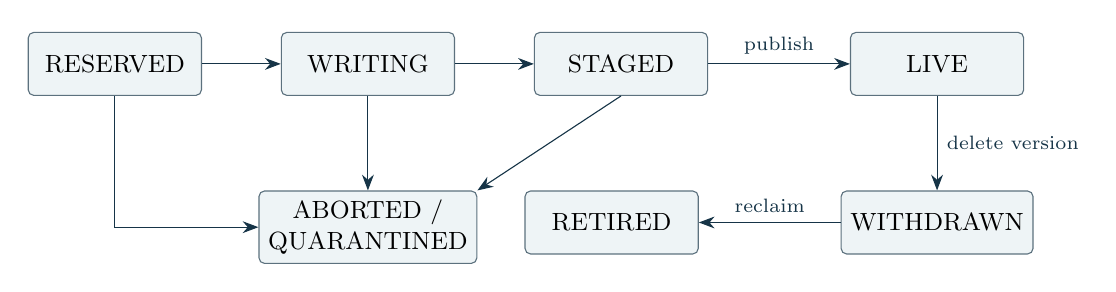
\begin{tikzpicture}[st/.style={draw=ink!70,rounded corners=2pt,fill=pale,align=center,minimum height=8mm,minimum width=22mm,font=\small},arr/.style={-{Stealth[length=2mm]},ink}]
\node[st] (res) {RESERVED};
\node[st,right=10mm of res] (wr) {WRITING};
\node[st,right=10mm of wr] (stg) {STAGED};
\node[st,right=18mm of stg] (live) {LIVE};
\node[st,below=12mm of live] (withdrawn) {WITHDRAWN};
\node[st,left=18mm of withdrawn] (retired) {RETIRED};
\node[st,below=12mm of wr] (ab) {ABORTED /\\QUARANTINED};
\draw[arr] (res) -- (wr);
\draw[arr] (wr) -- (stg);
\draw[arr] (stg) -- node[above,font=\scriptsize]{publish} (live);
\draw[arr] (live) -- node[right,font=\scriptsize]{delete version} (withdrawn);
\draw[arr] (withdrawn) -- node[above,font=\scriptsize]{reclaim} (retired);
\draw[arr] (res.south) |- (ab.west);
\draw[arr] (wr) -- (ab);
\draw[arr] (stg.south) -- (ab.north east);
\end{tikzpicture}
\caption[Version lifecycle]{Key deletion changes the object head to a separate delete marker; it does not change an older version's state. Version withdrawal and physical retirement require \rr{PUB-005}. Staged records may be durable without being publicly readable.}\label{fig:pubstates}
\end{figure}
\req{PUB-001}{R1-B}{T-08}{PostgreSQL controls logical namespace and visibility. Public bucket names and object keys \mustnot\ be used directly as filesystem paths.}
\req{PUB-002}{R1-B}{T-08, T-11}{Staging proceeds as follows. (1) \code{BeginEncryptedUpload} creates an intent with tenant, actor, subject, delegation, assigned object, logical-version, crypto-version and blob IDs, encrypted-attempt ID, expected generation/current version, metadata revision and idempotency key. (2) Authorize create or new-version and assign protected metadata, including the bucket's encryption mode. (3) In client mode the client constructs the exact bound ciphertext, signed descriptor and one independent envelope per object or unit and recipient; in server mode the storage role encrypts the uploaded plaintext under \rr{SSE-001} and \rr{SSE-005} with a data key obtained under \rr{SSE-003}, and there are no client descriptors or envelopes. (4) \code{FinalizeEncryptedUpload} validates exact identifiers, format, ciphertext digest/length and, in client mode, signatures and envelope references, obtains the backend durable receipt, and requires every initial envelope to satisfy the same caller-share/create and target-recipient read/receive-key checks as \code{PublishRecipientEnvelope} under \rr{KEY-012} and \rr{RES-009}. Target eligibility uses the trusted intended committed state within this upload plan, never a staged-data read grant. The version and its envelopes remain unpublished until the complete fresh commit succeeds. No client-mode upload route accepts a payload decryption key.}
\req{PUB-003}{R1-B}{T-08, T-11}{Commit obtains a fresh decision for object publication and every initial envelope. Under \rr{DAT-007}, one transaction checks expected generation/current version, metadata, caller and target-principal revisions, recipient-key state, delegation, policy epoch, recovery incarnation, decision expiry and conditional-write preconditions. A missing, stale or misbound check aborts. It atomically publishes the version and approved envelopes, updates the head, consumes the intent and appends audit/outbox records. The same boundary publishes newly staged document units under \rr{DOC-002}. Initial envelopes retain all \rr{KEY-012} checks; success requires the durability barrier.}
\req{PUB-004}{R1-B}{T-08}{Only a committed LIVE version is eligible for ordinary reads. A durable STAGED catalog record, finalized backend blob or failed commit grants no visibility; pending versions and envelopes remain inaccessible through every route.}
\req{PUB-005}{R1-B}{T-08}{Key deletion publishes a separate current-head delete marker and advances the head generation; historical LIVE versions remain readable only with historical rights. Explicit version deletion checks version-delete permission, retention and references, then durably changes that version to WITHDRAWN and schedules reclamation. Deleting the current version also leaves a head marker, never restores an older version. Physical removal follows the durable withdrawal and fresh retirement guards; only confirmed removal marks RETIRED.}
\req{PUB-006}{R1-B}{T-08}{Garbage collection uses catalog references, intents, withdrawals and a grace period; file age alone is insufficient. Reconciliation is idempotent across blob finalization and catalog commit. Expired RESERVED, WRITING or STAGED attempts can be aborted under expected-state checks. Restore reconciles catalog and blobs or quarantines mismatches, and reopens access only under \rr{AVL-008}.}
\req{PUB-007}{R1-B}{T-08}{\code{If-Match} and \code{If-None-Match} apply to the committed logical version and its documented ETag, not to a staging file. Conflicting commits serialize with row locks or compare-and-swap and a fixed lock order, and two concurrent overwrites \mustnot\ both publish against the same obsolete expected generation. An ETag is an opaque identifier and is not promised to be an MD5; the server stores ciphertext checksums only, in either mode. A plaintext digest, if needed by a client, stays inside its encrypted metadata and is verified locally.}
\req{PUB-008}{R1-B}{T-08}{An upload follows RESERVED, WRITING, STAGED and LIVE; any pre-LIVE state may end in ABORTED or QUARANTINED. Explicit version deletion follows LIVE to WITHDRAWN to RETIRED. Delete markers belong to the object-head history, not this version lifecycle. Transitions use expected-state checks, and no state change retargets immutable bytes (Figure~\ref{fig:pubstates}).}
\req{PUB-009}{R1-B}{REV}{The first release does not claim regulatory WORM or Object Lock compliance.}

\subsection{Object backend contract}
\begin{lstlisting}
// Logical contract. All requests carry verified workload bindings.
type ObjectBackend interface {
    Begin(ctx context.Context, req BeginRequest) (StagedWriter, error)
    Finalize(ctx context.Context, req FinalizeRequest) (DurableReceipt, error)
    Open(ctx context.Context, req ReadRequest) (BlobReader, error)
    Remove(ctx context.Context, req RetireRequest) (RemovalReceipt, error)
}
\end{lstlisting}
\req{BKD-001}{R1-B}{T-08, T-15}{\code{Begin} binds operation, tenant, blob and placement. \code{Finalize} checks exact length and digest and returns a durable receipt only after the backend's qualified durable completion condition: for the R1 single-node store, the required file and directory flushes after an exclusively created temporary file is fully written and verified; for a later backend, its own qualified acknowledgement bound to the immutable object identity and verified content. A successful network send alone is not a durable receipt. Repeating the same identity and content is idempotent, and the same blob ID with different bytes rejects. A timeout is an unknown result reconciled by operation identity, not an assumed failed write. \code{Open} exposes exact immutable bytes, and \code{Remove} accepts only a current catalog-authorized retirement plan. The caller owns stream close, cancellation and logical publication.}
\reqn{BKD-002}{R1-B}{T-08}{R1 runs on our own single-node blob store on local disk behind this contract (decision D-02). It writes each blob to an exclusively created temporary file, checks length and digest, flushes the file and its directory, and only then returns the durable receipt; the catalog, not the file system, decides visibility. It receives only ciphertext, from the client in client mode or from the storage role's encryption in server mode, and no other role has direct file access. R1 makes no zero-loss claim for blob content (N-08): losing the node loses blobs written since the last backup. A later backend (the replicated store of Part~5, or another store qualified under \rr{BKD-004}) replaces it without changing client policy semantics. Volume encryption supplements payload encryption and gives no platform role a payload decryption key.}
\req{BKD-003}{R1-B}{T-08}{The local backend uses service-owned directories, restrictive permissions, descriptor-relative safe file operations and symlink and traversal protection. Finalized blobs are immutable, and file and required directory metadata are flushed before a catalog transaction publishes a LIVE reference. Storage clients have no direct filesystem or backend credentials.}
\req{BKD-004}{R1-B}{T-08}{A different backend implements the same interface and needs its own consistency and durability tests. It does not duplicate user-facing policy combination in a second storage engine.}

\reqn{BKD-005}{R1-B}{T-08, T-18}{Payload encryption is mandatory from R1-B in both modes (\rr{ENC-001}). A server-mode upload is encrypted by the storage role before any byte reaches a staged blob, temporary file or spill (\rr{SSE-005}). A client-mode upload declares the approved encrypted format, supplies its signed binding and is produced by a qualified encrypting client. Payloads remain ciphertext in unpublished uploads, temporary files, spill, finalized blobs, replicas and backups, and no route stores payload plaintext; no server path decrypts a client-mode payload. Backend and volume encryption also protect persistent server records, opaque envelopes, wrapped keys and ciphertext, with an approved configuration, verification method and documented drift-detection bound. For client mode, a declaration or signature proves origin and binding, not that arbitrary maliciously supplied bytes were encrypted correctly; the cryptographic guarantee assumes the qualified client follows the format, and the server cannot prove payload AEAD validity without a key and does not claim to do so. Unsupported or missing profiles reject publication.}

\subsection{Documents and text units in the storage core}
Native document and text-unit endpoints are part of R1-C in both modes. They call the same resolver and delivery path later used by MCP; a document is a catalog projection over independently protected encrypted units, not an MCP-owned resource.
\req{DOC-001}{R1-C}{T-06, T-08}{A document version has a canonical manifest identifying its exact unit membership, unit/object versions, ciphertext digests and format, and declared extraction and normalization versions. Its digest is computed over the canonical core of unit entries before per-unit descriptors or signatures are added, avoiding self-reference. In client mode the manifest is uploader-signed, and each deliverable unit has an uploader-signed descriptor binding tenant, document/version, the opaque manifest digest, unit/version, ciphertext digest and crypto profile; the server verifies signatures and cross-references at publication, and a subset client verifies its descriptors without receiving the hidden full manifest. In server mode the storage role builds the manifest and unit bindings from the uploaded text and records them in the catalog with the authenticated uploader; there is no client signature.}
\req{DOC-002}{R1-C}{T-08}{New document units remain STAGED, with durable receipts and nonpublic catalog records, until the document transaction atomically publishes their LIVE versions, permitted envelopes, manifest and protective references. Already-published units may be referenced after current checks. In client mode a reused unit needs new document-specific descriptors and recipient envelopes prepared by an authorized client holding the unit key, and the server cannot create missing envelopes; in server mode reuse needs no client key, and the storage role binds the reused unit to the new manifest. Reuse preserves the immutable unit ciphertext. Every referenced unit must be LIVE at the transaction outcome, and incomplete ingestion is never exposed through raw, envelope or plaintext APIs. The parent and all affected units use the same authority fence and publication preconditions; retirement honors their references.}
\req{DOC-003}{R1-C}{T-06}{The qualified client in client mode, or the storage role in server mode, splits content at authorization boundaries into stable sections, paragraphs or independently protected entries and encrypts each unit with a separate payload key. Re-splitting creates a new document version. Protected access labels and revisions remain separate mutable server records; label changes alone do not change payload bytes, confer a missing recipient envelope or release a key.}
\req{DOC-004}{R1-C}{T-09}{The initial ingestion profile accepts bounded UTF-8 text and Markdown with a recorded normalization scheme. In client mode, parsing, extraction, segmentation, classification proposals and encryption occur on the client, never in the storage or MCP server, and the server checks signed declarations, sizes, references and uploader authority but cannot verify plaintext extraction quality or label correctness. In server mode the storage role applies the same bounded profile and normalization scheme to the uploaded text and keeps no extraction cache. Additional formats need a separately qualified extractor with complexity limits and source-to-text mapping. Neither mode classifies content on the server. There is no server converter, plaintext indexing worker or embedding-provider fallback.}
\req{DOC-005}{R1-C}{T-06}{A text collection or conversation uses the same unit model through \code{text.entry}; no separate transcript authorization store exists. Manifests, text units, source references and policy metadata are tenant-bound catalog records, and unit IDs are not bearer permissions.}
\req{DOC-006}{R1-C}{T-06}{Document permission to enumerate or read units does not grant every unit, recipient envelope or key release. Actor, subject and delegation checks apply to the parent, selected units and envelope recipient. The original file and its separate key need explicit complete-content permission under \rr{CNT-003}; this is never inferred from a unit read. Raw, preview, thumbnail, version, manifest, envelope and plaintext routes preserve that boundary; in client mode no plaintext raw-download route exists, and in server mode the original-file read is the only plaintext raw route.}
\req{DOC-007}{R1-C}{T-06, T-09}{An explicit unit-ID request requires every requested disclosure to be allowed; otherwise it returns a generic denial. An authorized-subset operation returns only permitted units with an opaque continuation: their plaintext in server mode, or the encrypted units, their signed descriptors and separate authorized recipient envelopes in client mode. In client mode each envelope context names exactly one object or unit version and one recipient, and the qualified envelope plaintext contains exactly that unit's keyset; batching never creates an aggregate opaque multi-unit key bundle. The server checks the outer identity and grants; the recipient verifies the single-unit keyset format after unwrapping, and the server cannot inspect HPKE plaintext or prove an authorized malicious sender has not hidden other material inside it. In server mode each unit is decrypted under its own released data key. Responses expose no hidden IDs, positions, counts or placeholders. The full manifest is returned only when all contained metadata may be disclosed, and in client mode sensitive titles and text stay encrypted for the recipient.}
\req{DOC-008}{R1-C}{T-06}{Streaming-AEAD segments and HTTP byte ranges are not independent authorization units. If different spans need different rights they are split into separate units before publication.}

\subsection{Labels}\label{sec:labels}
Authorization needs a trusted classification for every unit. Authorized labeling and collection defaults suffice for the baseline; a classifier in an authorized client is optional. The server does not classify content: in client mode it cannot read it, and in server mode it does not infer labels from it. Neither an untrusted client field nor a model-generated label is authoritative.
\reqn{LAB-001}{R1-C}{T-09}{Every published unit carries a protected classification label from the tenant's label order. Publication of an unlabeled unit is rejected.}
\reqn{LAB-002}{R1-C}{T-09, T-21}{A label comes from, in order of precedence: (1) explicit labeling by an authorized principal within their delegation ceiling and at or above the collection's floor; (2) the collection or bucket default; (3) a signed proposal from a registered client-side classifier, which is advisory until accepted under (1). Client-supplied and model-generated labels are never applied directly.}
\reqn{LAB-003}{R1-C}{T-09}{A unit whose label cannot be determined takes its collection's most restrictive default, and every collection declares one.}
\reqn{LAB-004}{R1-C}{T-09}{Lowering the stored label of a unit or derived output is an explicit \code{relabel} action with its own audit record and, by default, an approval. The effective label of a derived output cannot go below its lineage maximum unless a \code{relabel} allow for that output says so (\rr{DRV-007}). Raising a label is an ordinary \code{label} action.}
\reqn{LAB-005}{R1-C}{T-09}{A label change advances the affected access revision and invalidates dependent derived-output authority under \rr{DRV-009}. Decisions, disclosure plans, server-mode key releases and stream leases bind that freshness state (\rr{DEC-006}, \rr{CNT-008}). Payload re-encryption is not required.}

\subsection{Share grants}\label{sec:grants}
A share grant lets a principal name another principal who may read a resource, within what policy allows. It is an authority fact that rules can test, never a permission by itself, and it works in both encryption modes.
\reqn{SHR-001}{R1-B}{T-24}{Recording and removing a share grant are registered, audited operations that need \code{share} on the resource. A grant names one bucket, object, document version, unit, entry or derived output; one grantee principal of the same tenant; actions from the target type's read set (\code{read}, \code{stat} and \code{discover} on an object; \code{read-units} and \code{discover} on a document version; \code{read} on a unit or entry; \code{deliver} on a derived output; \code{list} on a bucket); and an expiry no later than the grantor's own delegation. A grant to an unknown, disabled or other-tenant principal, for any other action, or beyond the grantor's delegation is rejected.}
\reqn{SHR-002}{R1-B}{T-01, T-24}{The unexpired grantees of a resource, with their granted actions, are visible to policy as \code{resource.attributes.shared_with}. Only a business rule that tests that attribute turns a grant into an allow; without such a rule a grant has no effect (default deny), and platform ceilings, labels and clearances still apply. Recording, expiring or removing a grant advances the resource's access revision, so decisions, plans, key releases and stream leases bound to the earlier state are invalidated (\rr{DEC-006}, \rr{CNT-008}).}
\reqn{SHR-003}{R1-B}{T-24}{In server mode an honored grant is enough for the storage role to decrypt for the grantee after the ordinary checks. In client mode it makes the grantee eligible under the target-recipient checks of \rr{KEY-012} but supplies no key: a client holding the data key must still publish the grantee's recipient envelope. A grant on a document reaches its units only where a rule says so, and unit checks remain per unit (\rr{DOC-006}).}

\subsection{Disclosure}
\req{DSC-001}{R1-C}{T-09}{Disclosure resolves the exact document/manifest, selected units and current authority, including transitive lineage dependencies under \rr{DRV-009}; obtains the complete parent/unit checks and, in client mode, the recipient-envelope checks; then admits that immutable plan under \rr{DAT-007}. In client mode only its authorized ciphertext, descriptors and existing envelopes are returned, and verification and decryption remain client-side. In server mode only the authorized units' plaintext is returned, each decrypted under its own released data key.}
\req{DSC-002}{R1-C}{T-09}{The server authorizes plaintext, ciphertext and envelope delivery before any of them enters a response, shared cache or downstream route. It returns server-mode plaintext only to the authenticated caller of an authorized read and never sends content to a model, reranker or embedding API on its own initiative; it never returns client-mode plaintext. A client that receives plaintext or decrypts an authorized package owns subsequent plaintext handling. Post-generation redaction and model instructions cannot substitute for the server's delivery checks or make client plaintext recallable.}
\req{DSC-003}{R1-C}{T-09}{The platform records plaintext, ciphertext and envelope delivery and server-mode key releases with exact unit/version/recipient identities and hashes, not plaintext prompts, raw keys or documents. A managed client may submit signed outcome evidence for its own optional model calls, but the server distinguishes that report from a platform-observed event and does not claim to have observed the client's plaintext use.}
\req{DSC-004}{R1-C}{T-09}{The same final unit and recipient checks apply to every disclosure surface, including preview objects, citations, notifications and subscriptions. The server emits only authorized metadata, encrypted payloads or the server-mode plaintext of authorized units. Client-generated previews and snippets are separate resources or local views; an unsupported surface is disabled.}
\req{DSC-005}{R1-C}{T-09}{Query caches are bound to tenant, authority, version and epoch and \mustnot\ reuse a result computed for a broader user for a narrower one. No raw totals or structural positions reveal denied units.}
\req{DSC-006}{R2}{T-09}{Once an authorized client receives server-mode plaintext, or a usable envelope while holding its private key, the server cannot constrain where that client sends plaintext. A destination restriction may limit which registered recipient receives content or an envelope; it does not enforce subsequent use by an arbitrary client. Any stronger managed-client promise requires a separately qualified runtime boundary and excludes that runtime's compromise. The baseline has no server-side plaintext model-proxy route.}

\subsection{Search}
\req{SRH-001}{R1-C}{T-09}{Server search is restricted to authorized catalog metadata whose visibility is explicit: tenant, permitted aliases, approved policy attributes and opaque object/version references. It performs no plaintext full-text, semantic or embedding search in either mode. After an authorized read (and, in client mode, decryption), the recipient client may search locally; its text query need not leave the client.}
\req{SRH-002}{R1-C}{T-09}{Plaintext and embedding indexes are client-side state and remain outside the server storage boundary. A qualified client protects any persistent local index with its local key custody and excludes unauthorized or undecryptable units. The server stores no plaintext snippets, embeddings or extraction cache; encrypted client indexes, if uploaded, are ordinary encrypted objects and are not server-searchable plaintext.}
\req{SRH-003}{R1-C}{T-09}{The baseline server has no remote text-search, reranking or embedding integration. A client that sends decrypted content to such a service makes an additional plaintext disclosure outside baseline storage enforcement; a managed-client extension must declare and qualify that boundary. Searchable encryption, private search and server decryption are not implied by metadata discovery.}
\reqn{SRH-004}{R1-C}{T-09}{Result values, ordering, scores and totals returned to a caller depend only on candidates that caller is authorized to see. Page shape (short or empty pages) and latency can reflect scan work over hidden candidates; they are bounded by the scan budget and tenant limits, but the platform does not claim that pagination is noninterfering with respect to hidden candidates.}

\subsection{Derived outputs and declassification}\label{sec:derived}
A client-created projection, extraction or model answer is uploaded as a new resource, encrypted under its bucket's mode. R1-C enforces labels and declared lineage for registered derived resources. These controls rely on qualified cooperating clients accurately describing their computation; the server cannot prove provenance, whether it holds ciphertext (client mode) or sees the output plaintext (server mode). Possession of plaintext by an authorized client remains a trust boundary.
\reqn{DRV-001}{R1-C}{T-09, T-21}{A managed or cooperating client that creates a derived object declares lineage naming all input units the operation received. In client mode it signs that lineage and encrypts the result before upload; in server mode it declares lineage in the authenticated upload request, bound to the caller's decision, and the storage role encrypts the result. The server validates signer or uploader authority, references, bounds and cycles. Citations do not narrow declared lineage. Because the server does not observe the computation, it cannot prove that a malicious client declared every source or that an uploaded object was independently created.}
\reqn{DRV-002}{R1-C}{T-09}{For a registered derived object, delivery requires the normal object checks (and, in client mode, envelope checks) and either (a) recipient read permission on every declared lineage unit or (b) an explicit \code{declassify} decision for that exact output, version and recipient. In client mode the owner or authorized custodian client must have created the recipient envelope, and a policy allow cannot synthesize one; in server mode the storage role decrypts for the recipient after the same checks. Declassification authorizes that delivery only and does not lower the stored label.}
\reqn{DRV-003}{R1-C}{T-09}{The managed client binds the intended recipient and conservative lineage before publishing the encrypted output. The server enforces the registered bindings without inspecting wording or inferring whether plaintext leaked. This is a provenance-based delivery rule for cooperating clients, not information-flow proof against an authorized malicious client.}
\req{DRV-004}{R2}{T-09}{Optional AI submission runs in a client or explicitly trusted managed client runtime. That client obtains permitted units (plaintext in server mode, or encrypted units and envelopes it verifies and decrypts locally in client mode) and constructs its own model request. A server may authorize the proposed recipient/model metadata, but never builds a plaintext prompt or forwards content to a model. A managed profile binds destination and parameters; baseline storage makes no claim to police arbitrary client networking.}
\reqn{DRV-005}{R2}{T-09}{The baseline rejects a request to perform server-side \code{use-in-model} without client read capability; it has no plaintext execution path for it. A future managed-client profile may distinguish an end user from a separate authorized execution recipient, but must qualify that client's custody, output encryption and recipient-specific declassification before being enabled. For client-mode content it cannot be implemented by giving the storage or MCP server a decryption key.}
\reqn{DRV-007}{R1-C}{T-09, T-21}{The effective server label of a registered derived output is at least the highest effective label in its declared lineage. A collection default acts as a floor, so the effective label is the maximum of the collection default and the lineage maximum. Only an explicit \code{relabel} allow for that output can lower it, and the effective label is the one used when the output is reopened and when a context mark is updated.}
\reqn{DRV-008}{R1-C}{T-09, T-21}{Disclosure to one recipient and relabeling are separate authorizations. A \code{declassify} allow is bound to output, version and recipient and records the label reported to a qualified managed client for flow control; absent an explicit lower label, that is the lineage maximum. Lowering the stored label for everyone is a \code{relabel} action (\rr{LAB-004}).}
\reqn{DRV-009}{R1-C}{T-09, T-13, T-21}{Derived-output authority includes its complete transitive lineage. A source access, label, lifecycle or relevant declassification change invalidates dependent decisions and leases even when output bytes and revisions are unchanged. The implementation may use dependency revisions, a conservative epoch or transactional propagation, but must qualify equivalent freshness under \rr{DAT-007}, bounded traversal and cycle rejection. New delivery recomputes effective authority; ongoing delivery follows \rr{CNT-008}. Test chained derivation and a source change during an output stream.}
\req{DRV-006}{R2}{REV}{An AI provider receiving plaintext from a client is outside the storage boundary. Client/provider retention, training and onward disclosure are not controlled by the storage cryptography in either mode. Managed-client lineage records describe declared provenance, not proof against hidden inputs, malicious client behavior or sensitive inference.}

\subsection{MCP as a later content client}
The R2 MCP service is an authenticated facade over the same content API. It preserves user and delegation authority and returns the exact versions and projections a native client can obtain. For server-mode content that is plaintext, which the storage role decrypts after the same checks, so a generic MCP client can read it. For client-mode content it is the encrypted package: a qualified client SDK or local bridge verifies the descriptors and decrypts with keys held on the client side of that boundary, a generic MCP client does not automatically understand that representation, and capability negotiation either selects the qualified format or reports it unsupported. No compatibility mode returns client-mode plaintext from the server.
\begin{longtable}{@{}P{0.22\textwidth}P{0.27\textwidth}P{0.32\textwidth}P{0.08\textwidth}@{}}
\caption{Later MCP service mappings to content operations}\label{tab:mcpops}\\
\toprule MCP operation & Required action model & Returned representation & Phase\\\midrule\endfirsthead
\toprule MCP operation & Required action model & Returned representation & Phase\\\midrule\endhead
\code{documents.search} & Authorized metadata discovery only & Permitted references and metadata; no server text snippets, embeddings or plaintext query processing & R2\\
\code{documents.read} & Parent and unit read, plus all recipient-envelope checks in client mode & Server mode: plaintext of the permitted units. Client mode: selected ciphertext, signed unit descriptors and existing recipient envelopes; local decryption & R2\\
\code{text.read} & Collection/entry and exact-version read, plus recipient checks in client mode & The same unit representation as \code{documents.read}; no unguarded text endpoint & R2\\
\code{resources/list}, \code{resources/read} & Same discovery and read checks as tools & Registry-bound references and the same representation as the native read; no direct backend or file access & R2\\
\code{documents.export} & Complete mapping of Table~\ref{tab:keyops} & Client mode: ciphertext and envelopes for an approved compatible recipient, with no server rewrapping or decryption. Server mode: plaintext of a permitted complete export & R2\\
\bottomrule
\end{longtable}
Optional AI assistance is a client workflow after an authorized read. The baseline MCP service exposes no \code{ai.ask} operation that receives or constructs plaintext context; any managed-client model integration needs its separately qualified authority and disclosure boundary.

\subsection{Sizing and scaling}
\reqn{SIZ-001}{R1-B}{T-22}{Qualification reports measured object-service capacity in R1-B for both modes: server-mode encryption and decryption throughput and data-key wrap and unwrap rates, and client-mode ciphertext transfer with client encrypt/decrypt costs; then unit and recipient-envelope fan-out for the reference documents in R1-C. R2 adds the independently deployed MCP service. Measurements separate server payload cryptography, ciphertext throughput and signature checks from client HPKE wrapping/unwrapping and payload AEAD work.}
\req{SIZ-002}{R1-B}{T-22}{The \code{storage} role scales independently with bounded requests, payload streams, server-mode encryption work, upload/read concurrency, buffer memory, signature-verification work and tenant byte budgets; the \code{keys} role scales with key releases. Decision replicas and backend capacity are qualified with \rr{AVL-007}; adding frontends does not imply unlimited catalog throughput. R1-C adds bounded unit and envelope fan-out and metadata discovery. The R2 \code{mcp} role has its own replica set and identity and calls the same content API. Client compute and local indexes scale at the client; no server permission database, evaluator or plaintext cache is added for MCP.}
\begin{longtable}{@{}P{0.28\textwidth}P{0.44\textwidth}P{0.18\textwidth}@{}}
\caption{Sizing quantities (formulas; values are measured, not assumed)}\label{tab:sizing}\\
\toprule Quantity & Measurement or formula, with $u$ units per document and $c$ search candidates & Release\\\midrule\endfirsthead
\toprule Quantity & Measurement or formula, with $u$ units per document and $c$ search candidates & Release\\\midrule\endhead
Object-service capacity & Object-size distribution, concurrent streams, read/write throughput, catalog commit rate, backend latency and bounded memory per request & R1-B\\
Decision batches to read a whole document & $\lceil k/50 \rceil$, where $k$ includes the parent, $u$ unit checks and every required recipient-envelope check & R1-C\\
Decision batches per metadata page & $\lceil c/50 \rceil$ before any prefilter (\rr{CNT-007}) & R1-C\\
Blobs, catalog rows per ingest & $u$ blobs, $u$ unit rows, 1 manifest & R1-C\\
Recipient envelopes (client mode) & Up to $u \times r$ client-created HPKE envelopes for $r$ authorized recipients; server stores and authorizes delivery only & R1-C\\
Client cryptographic work (client mode) & $u$ independent payload encryptions at ingest; selected-unit envelope unwraps and payload decryptions at recipients & R1-C\\
Server cryptographic work (server mode) & $u$ data-key wraps and payload encryptions at ingest; one key release and payload decryption per delivered unit & R1-C\\
Durable receipts per publication & Backend-defined; 2 per immutable blob with the custom store & R1-B, R3\\
Reference documents & $u = 10$, $u = 1{,}000$ and $u = 10{,}000$ & R1-C\\
\bottomrule
\end{longtable}

\section{Payload encryption, key custody and authorized delivery}\label{sec:custody}
Every stored payload is encrypted. A bucket's encryption mode (\rr{ENC-001}, decision D-12) decides who encrypts it and who can decrypt it. In \term{server mode}, the default, the storage role encrypts each version under a fresh data key that is wrapped by a tenant key-encryption key (KEK) held only by the \code{keys} role, and decrypts for a reader only after the \code{keys} role has released that data key under a fresh signed decision for the exact operation. In \term{client mode}, which a bucket opts into, clients encrypt content before upload and decrypt it after download, and no platform role can read it. R2 MCP follows the same modes: it returns server-mode content as plaintext after the same checks and client-mode content as encrypted packages. TLS protects every connection in both modes, and payloads remain ciphertext in backing stores and backups.

For client-mode content, no platform role receives plaintext payloads, raw data keys or recipient private keys. The \code{keys} role is then an authorization and envelope-delivery service: it stores and returns opaque, client-created recipient envelopes and cannot unwrap them, rewrap one for another user, or recover plaintext. For server-mode content it holds the tenant KEKs and wraps and unwraps data keys only under signed decisions; it never sees blobs or payload plaintext. Independently authored Go code integrates qualified streaming AEAD, HPKE and signature libraries; it does not invent cryptographic primitives.

\subsection{Encryption modes}
\begin{longtable}{@{}P{0.11\textwidth}P{0.24\textwidth}P{0.30\textwidth}P{0.25\textwidth}@{}}
\caption{Encryption modes}\label{tab:modes}\\
\toprule Mode & Encrypts & Decrypts for a reader & Sharing\\\midrule\endfirsthead
\toprule Mode & Encrypts & Decrypts for a reader & Sharing\\\midrule\endhead
\code{server} (default) & The storage role, with a fresh data key per version wrapped under the tenant KEK & The storage role, after the \code{keys} role releases the data key under a fresh decision for the exact operation & Policy decides who reads, including through share grants (\rr{SHR-002}); no recipient key is needed\\
\code{client} (opt-in) & The uploading client, before upload & Only clients holding a recipient envelope and its private key & Policy allows the reader, and a key-holding client publishes the reader's envelope\\
\bottomrule
\end{longtable}
\reqn{ENC-001}{R1-B}{T-06, T-23}{Every bucket has exactly one encryption mode, \code{server} or \code{client}, set through the authorized control API when the bucket is created; \code{server} is the default. There is no plaintext mode. The mode is protected bucket metadata and is visible to policy as \code{resource.attributes.encryption} on the bucket and on every resource stored in it, including objects, document versions, units, entries and derived outputs, so that a business rule or platform ceiling can require a mode, for example for a label. Changing it is a registered operation that needs \code{manage} on the bucket and may need an approval; it applies only to uploads begun after the change commits.}
\reqn{ENC-002}{R1-B}{T-23}{Each immutable version records the mode it was published under and keeps it. A client-mode version is never read, delivered, exported or migrated through a server-held key, and a server-mode version never takes a client-created recipient envelope or client signature in place of its server binding. A route for one mode refuses a resource of the other mode with a stable error, after the existence checks of \rr{CNT-004}. A version moves to the other mode only as a new version: an authorized principal reads it through its own mode and writes it again under the ordinary write checks.}
\reqn{ENC-003}{R1-B}{REV}{Documentation, administrative listings and audit state which mode applies to each bucket and version. The guarantee that no platform role can read content is claimed only for client-mode versions; server-mode content carries non-guarantee N-09. Upgrading a deployment from a release without modes places its existing buckets in client mode, so already-published content keeps its custody.}

\subsection{Server mode: platform-held keys}
Server mode trades the client-custody guarantee for reach: any authenticated client, including a generic MCP client, can read what policy allows, and no reader needs a recipient key. Its protection is the access decision, enforced inside the authority fence at every key release, and the separation of KEKs (\code{keys} role) from blobs and plaintext (storage role).
\reqn{SSE-001}{R1-B}{T-23}{In server mode the storage role encrypts each object version, unit version, original file and derived-output version with a fresh data key under the qualified streaming AEAD of \rr{CRY-002}. The AAD binds tenant, object, logical version, crypto version, blob, suite, format and the server mode under a domain identifier distinct from the client-mode AAD of \rr{CRY-003}, so ciphertext copied to another identity or presented as client-mode content fails authentication. Data keys are never shared across tenants, objects, units or versions, and no bucket-wide or document-wide data key exists.}
\reqn{SSE-002}{R1-B}{T-18, T-23}{Each tenant has versioned key-encryption keys held only by the \code{keys} role. The catalog stores each server-mode data key only wrapped under a KEK, with the KEK version and a binding to the same identity as the AAD. No other role holds a KEK, and the \code{keys} role never holds blobs, ciphertext streams or payload plaintext. KEK rotation adds a version and rewraps data keys inside the \code{keys} role without changing ciphertext; a retired version is kept until no wrapped key refers to it. Production KEK custody is decision D-13; until it is closed, KEKs are development key files protected like other local key files, and no production payload is accepted in server mode.}
\reqn{SSE-003}{R1-B}{T-13, T-23}{The \code{keys} role generates and wraps a data key only against a signed decision for the exact write, naming its upload intent, and unwraps one only against a single-use signed decision for the exact read, export or disclosure operation and version. It verifies that decision inside the ordering fence of \rr{DAT-007} with the same bindings as recipient-envelope delivery: audience and exact check set, current identity and revisions, policy epoch, recovery incarnation, approval, the head state of a current-version read and, for an original file, every unit check of \rr{CNT-003}. A missing, stale or misbound decision releases no key. Every read obtains a fresh release, so revoked authority takes effect at the next admission without retiring any envelope. Each wrap and unwrap is audited with resource, version, operation and decision identifiers, KEK version and outcome, never key material.}
\reqn{SSE-004}{R1-B}{T-19, T-23}{An unwrapped data key exists only in the memory of the \code{keys} role for one wrap or unwrap and of the storage role for one upload or read stream. It is never persisted, logged, cached across requests or returned to a client, and it never reaches the decision, MCP, tools or maintenance roles. Key buffers have an explicit owner and lifetime and are cleared after use as far as the runtime permits (\rr{KEY-007}). Server-mode plaintext is likewise kept out of logs, traces, dumps, temporary files and support exports.}
\reqn{SSE-005}{R1-B}{T-08, T-23}{A server-mode upload is encrypted as it arrives: plaintext never reaches a staged blob, temporary file or spill. The storage role records ciphertext digest and length and obtains the durable receipt before publication under the ordinary protocol (\rr{PUB-002}, \rr{PUB-003}). A retry with the same idempotency key returns the outcome of the attempt it names and cannot change bytes already staged or published; a restarted encryption uses a fresh data key and fresh version, crypto-version and blob identities (\rr{CRY-007}). On read the storage role decrypts authenticated segments in order and aborts the connection on an authentication, digest or stream-termination failure; it never reports a shorter plaintext as complete. Range reads remain unsupported.}
\reqn{SSE-006}{R1-B}{T-18, T-23}{Backups contain wrapped data keys with the catalog, never KEKs or unwrapped keys. Restore needs the KEK versions that the restored wrapped keys refer to, recovered separately under D-13. Reconciliation verifies that each referenced KEK version is present and quarantines server-mode versions whose keys cannot be unwrapped before admission reopens (\rr{AVL-008}). Final removal of a server-mode version destroys its wrapped data key; the content is unrecoverable once no retained backup holds that wrapped key, and the platform reports that point rather than claiming it earlier.}

\subsection{Client mode: client custody}
The rest of this part applies to client-mode versions unless a requirement names server mode. Each immutable object version has a fresh data key (keyset). In R1-C each separately protected text-unit version is an ordinary immutable object with its own fresh keyset. A client encrypts the payload under that keyset and wraps the keyset to each explicitly approved recipient public key using HPKE. The server stores ciphertext and opaque recipient envelopes with authenticated bindings. There is no shared bucket data key, server master decryption key or whole-document data key that unlocks independently protected units.

\begin{longtable}{@{}P{0.27\textwidth}P{0.63\textwidth}@{}}
\toprule Boundary (client mode) & Material and responsibility\\\midrule\endhead
Owner or authorized recipient client & Plaintext, its private keys and the data keys it can unwrap; encrypts, verifies and decrypts locally\\
Optional organization custodian client & An independently controlled client with an explicit recipient envelope; can recover or authorize new recipient envelopes only for versions it can already decrypt\\
Platform storage role & Ciphertext, signed descriptors and catalog bindings; verifies publication, access and durability without decrypting\\
Platform \code{keys} role & Opaque recipient envelopes and public-key records; authorizes publication and delivery without unwrap capability\\
MCP and tool services & Authorized encrypted packages and permitted routing metadata; no plaintext conversion or private-key custody\\
Backing storage and backups & Ciphertext and protected metadata; provider encryption is additional protection, not a substitute for payload encryption\\
\bottomrule
\end{longtable}
\req{CRY-001}{R1-B}{T-10}{Client encryption is the only payload custody profile of a client-mode bucket. There, missing, unknown, server-decryptable or unencrypted profiles reject publication, and neither an API flag nor a privileged server role can request plaintext storage or server-side decryption of a client-mode version. In either mode, profile, suite, format and mode are recorded for each immutable version and checked on every operation that reads or delivers it.}

\subsection{Payload cipher suite and immutable binding}
\req{CRY-002}{R1-B}{T-10}{The client SDK, and the storage role for server-mode content, use a qualified streaming AEAD (initial candidate: Tink AES-256-GCM-HKDF with 1 MiB segments). The library handles nonce generation, key derivation, segment authentication and final-segment marking; project code \mustnot\ reproduce its chunked encryption. The module checksum and format tests are pinned.}
\req{CRY-003}{R1-B}{T-10}{Payload additional authenticated data (AAD) binds the tenant, object, crypto version, cipher suite and format under a versioned domain identifier. The same binding appears inside each recipient key package, preventing substitution across those identities. Mutable display names, classifications and envelope generation are excluded so that authorized metadata and recipient changes do not rewrite payloads. AAD is authenticated, not confidential; secrets and personal data do not belong in it. The exact field encoding is retained in the companion \code{crypto-format-profile.tex} and is qualified with the client wire contract under \rr{RCP-007}.}

\req{CRY-004}{R1-B}{T-10}{A published client-mode version binds tenant, object, logical version and crypto-version IDs; suite and format; ciphertext digest and length; uploader signing identity; and signed ciphertext descriptor. Its envelope records additionally bind recipient fingerprint and key version, envelope generation, opaque HPKE ciphertext and the origin signature. Logical versions, crypto versions, recipient-key versions and envelope generations remain distinct. A server-mode version binds the same identities, suite, format, ciphertext digest and length, the authenticated uploader and its wrapped data key and KEK version (\rr{SSE-002}) instead of a client signature and envelopes.}
\req{CRY-005}{R1-B}{T-11}{Client-mode raw keysets and recipient private keys never enter platform APIs, logs, persisted records or process memory; only authorized clients handle them. Server-mode data keys follow \rr{SSE-004} and never leave the memory of the storage and \code{keys} roles. A public key or client-supplied opaque envelope is not authority to read, create or share a resource; the server checks the exact operation independently of possession of those bytes.}

\subsection{Client-generated keys and server envelope service (client mode)}
\reqn{KEY-001}{R1-B}{T-10, T-12}{Client mode uses flat recipient wrapping: the client generates a fresh data keyset for every immutable object version and, in R1-C, every protected unit version, then creates a separate HPKE envelope for each explicitly approved recipient. Every envelope contains exactly one keyset for one immutable object or unit version and one recipient; a batch is a container of independently authorized envelopes, never a multi-unit encrypted key bundle. Data keys are not shared across tenants, objects or versions. A document-level KEK hierarchy for client-mode keys is deferred under D-09; any later proposal keeps those KEKs solely in authorized clients, preserves independent unit release, and cannot give platform roles an unwrap capability for client-mode keys. The server-mode tenant KEK of \rr{SSE-002} is a separate profile and never wraps a client-mode key.}
\req{KEY-002}{R1-B}{T-11}{The envelope service authenticates the calling client or service and requires a signed decision for the exact delivery or publication operation. It resolves recipient fingerprints and envelope identities from the canonical registry and catalog, verifies current revisions, and returns only the exact stored envelope for that recipient. It never accepts a caller-provided key-server URL, unwraps an envelope, or substitutes a broader recipient.}
\req{KEY-003}{R1-B}{T-11}{Before encryption, an upload intent binds the stable object ID and allocates fresh logical-version, crypto-version and blob IDs for that encrypted attempt. Exact retries reuse those IDs and the identical ciphertext; a restarted encryption attempt requires a new intent with fresh version, crypto-version and blob IDs. The server validates ciphertext length and digest, signed descriptor, uploader authority, recipient bindings, durable receipts and publication preconditions; it cannot verify the inner AEAD tag, plaintext format, plaintext classification or whether an opaque envelope decrypts. Those properties depend on the authorized publishing client and are checked by receiving clients where possible. Outer format validation cannot prove that a malicious uploader encrypted arbitrary submitted bytes; the confidentiality guarantee assumes a trusted compatible publishing client, not truthful labels on hostile uploads. Pending ciphertext and envelopes are not eligible for general reads.}
\req{KEY-011}{R1-B}{T-10, T-11}{The client and server operations of client mode behave as in Table~\ref{tab:broker}. Their server operation names and API types \mustnot\ imply plaintext key generation, unwrap or rewrap. The server-mode key operations of \rr{SSE-003} are separate operations, named as such, and never accept or return client-mode key material.}
\reqn{KEY-012}{R1-B}{T-11}{Ciphertext access, recipient-envelope delivery and sharing are separate compound operations with the check sets of Table~\ref{tab:keyops}. The storage and envelope services verify the complete applicable signed result, exact operation and recipient bindings; absence of a required check denies. Initial envelopes supplied with an upload pass the same publication checks as later envelopes, including recipient-revision checks at commit. Publisher share/create checks use the authenticated publisher actor and subject; target read/read-units and receive-key eligibility use the server-resolved recipient principal through \rr{RES-009}. Each signed check names its evaluated principal and current identity revision. Initial-upload eligibility is evaluated for the exact planned published state bound to the intent, not as permission to read STAGED content. An eligibility result grants no delegation or present read authority; caller-supplied recipient attributes cannot replace authoritative resolution. R1-C applies the same checks to both the document boundary and every selected unit.}
\begin{longtable}{@{}P{0.30\textwidth}P{0.47\textwidth}P{0.13\textwidth}@{}}
\caption{Compound operations for encrypted content}\label{tab:keyops}\\
\toprule Operation & Required checks and bindings & Enforcer\\\midrule\endfirsthead
\toprule Operation & Required checks and bindings & Enforcer\\\midrule\endhead
Ciphertext read & \code{read} on the exact object version; for documents, parent \code{read-units} and \code{read} on every selected unit; permitted metadata projection & Storage\\
\code{GetRecipientEnvelope} & Caller read and envelope-release checks; separate target-recipient read/read-units and \code{receive-key} eligibility under \rr{RES-009}; exact recipient fingerprint and current revisions & Envelope service\\
\code{PublishRecipientEnvelope} & Publisher \code{share} on the exact object or document and selected units, plus envelope \code{create}; separate target-recipient read/read-units and \code{receive-key} eligibility; client-origin signature and exact ciphertext binding & Envelope service\\
Remote package export & \code{export} on the object or document version and \code{export-key} on each selected unit where applicable, in addition to the applicable read and envelope-delivery checks; only an already-created envelope for that recipient & Storage and envelope service\\
\bottomrule
\end{longtable}
\begin{longtable}{@{}P{0.29\textwidth}P{0.61\textwidth}@{}}
\caption{Client and envelope-service operations}\label{tab:broker}\\
\toprule Operation & Required behavior\\\midrule\endfirsthead
\toprule Operation & Required behavior\\\midrule\endhead
\code{BeginEncryptedUpload} (server) & Authorize create or new-version; bind stable object ID and allocate intent, logical-version, crypto-version and blob IDs; return parameters without generating or receiving a data key\\
\code{EncryptObjectVersion} (client) & Generate keyset; stream-encrypt with exact AAD; create recipient envelopes for independently verified approved public keys; sign ciphertext descriptor and envelope contexts\\
\code{FinalizeEncryptedUpload} (server) & Verify signature, intent, profile, ciphertext digest/length and durable receipt; apply the full initial-envelope checks. Publish at the authorized object commit, or retain document units STAGED until the atomic document commit\\
\code{GetRecipientEnvelope} (server) & Verify the full signed delivery decision and freshness; return the existing opaque client-created envelope with its origin evidence; record delivery audit\\
\code{CreateRecipientEnvelope} (client) & Obtain a usable existing envelope and verify source; authorize sharing; verify target fingerprint independently; unwrap locally and create a new HPKE envelope for the same data key and exact version; sign its context\\
\code{PublishRecipientEnvelope} (server) & Recheck publisher authority, target-recipient eligibility and both identity and recipient revisions at commit; verify client origin and bindings; atomically publish opaque envelope, generation and audit record\\
\code{RetireEnvelope} (server) & Authorize retirement; withdraw future delivery, advance revisions and record audit; preserve required recovery references without claiming to erase client copies\\
\bottomrule
\end{longtable}

An owner or organization custodian is a client connected to the same system, not a privileged server decryption role. It can create a new recipient envelope only if it already holds the corresponding private key or a usable data key. Approval alone cannot manufacture access to an existing encrypted version. If no such client is available, the share operation remains unavailable; there is no emergency server unwrap.

\subsection{Client key custody and failure handling}
\req{KEY-004}{R1-B}{T-10, T-12}{Recipient-key rotation is performed by an authorized client: decrypt an existing envelope locally, verify the newly approved recipient key, create and sign a replacement envelope, and publish it under the expected envelope and recipient revisions. The data key and ciphertext identity remain unchanged. The platform cannot rewrap it itself, and rewrapping the same disclosed data key does not revoke old access.}
\req{KEY-005}{R1-B}{T-10, T-12}{The client uses its approved private-key store and a qualified cryptographic library. Optional hardware or an organization-operated key service belongs to the explicitly trusted client custody boundary and is selected under D-08; it is not a platform KMS unwrap dependency. No platform identity has permission to use recipient private keys. Envelope encryption is randomized; retries reuse the persisted encrypted attempt and operation identity, not convergent encryption or caller-chosen nonces.}
\req{KEY-006}{R1-B}{T-10}{Inside HPKE, a versioned key package carries the exact payload binding and one library-serialized binary keyset, with explicit bounded lengths. The receiving client rejects inconsistent lengths, trailing bytes, unknown versions, keysets above 64 KiB, extra keys or keysets, and any suite, binding or streaming-AEAD-template mismatch before use. The exact field ordering and integer encodings are retained in \code{crypto-format-profile.tex}. Servers treat the package as opaque and enforce only outer encoding and size bounds; they cannot prove that a hostile publisher put only the declared key inside HPKE.}
\req{KEY-007}{R1-B}{T-19}{Clients protect keys and plaintext against logs, traces, dumps and support exports and restrict debugging of decryption processes. Raw key buffers have an explicit owner and lifetime, avoid strings and unnecessary copies, and are cleared when the API permits. Perfect zeroization of Go or library-managed copies is not promised. Server diagnostics contain only permitted metadata and opaque-envelope identifiers; TLS protects all client and service connections in addition to payload encryption.}
\reqn{KEY-013}{R1-B}{T-11}{Process and credential boundaries prohibit all platform roles, including storage, decision, MCP, tools, maintenance and envelope delivery, from receiving client-mode payload plaintext or client-mode data keys. For server-mode content only the storage role handles plaintext and unwrapped data keys and only the \code{keys} role handles KEKs (\rr{SSE-002}, \rr{SSE-004}); the decision, MCP, tools and maintenance roles receive neither. The client verifies both a client-mode package's origin and its own recipient binding before decryption. Deployments \mustnot\ host a plaintext-processing custodian or model inside the platform and describe it as client-only encryption.}
\reqn{KEY-014}{R1-B}{T-11, T-13}{Server caches contain only ciphertext, opaque envelopes or permitted metadata, never plaintext keysets, unwrapped data keys or server-mode plaintext. Every new delivery or key release still checks current identity, recipient status, resource and envelope revisions, policy epoch and expiry. Client key retention follows the client's explicit custody policy; the platform does not claim that a client-side cache expires cryptographically when a grant or server lease expires.}
\reqn{KEY-015}{R1-B}{T-11, T-13}{A missing recipient envelope, unavailable client private key, failed signature or AEAD validation, stale authority, or unavailable authorization dependency prevents the corresponding delivery or decryption. A client-mode version never falls back to a server-held key (\rr{ENC-002}), another recipient, an older weaker profile or plaintext transfer, and a server-mode read whose key release fails returns no content. Client-side key-store failure does not cause private keys to be uploaded to the platform.}

\subsection{Client decryption, streaming and copy}
\req{CRY-006}{R1-B}{T-10}{The client releases plaintext only after verifying its signed origin and exact ciphertext digest and length. The baseline therefore receives the complete ciphertext into bounded, access-restricted encrypted-content storage before decrypting it as authenticated segments; it rejects oversized objects, insufficient temporary capacity, incomplete transfers and digest failures without releasing plaintext. Temporary ciphertext is cleaned up under the client custody policy. An alternative streaming profile needs equivalent authenticated origin binding and separate qualification. Overall success additionally requires valid AEAD stream termination. Wrong AAD or key, corruption, segment reordering, duplication, truncation and forged final segments fail. Memory and concurrent work remain bounded. Qualification includes temporary-storage demand and time to first plaintext; server leases govern delivery, not subsequent use of retained bytes or keys.}
\req{CRY-007}{R1-B}{T-10}{Retrying an upload resends identical ciphertext and envelopes for the same encrypted attempt. Restarting encryption requires a new intent and fresh logical-version, crypto-version and blob identities, together with a fresh keyset; it cannot overwrite an earlier attempt or change the bytes associated with an existing idempotency identity. Server-mode retries follow \rr{SSE-005}. The baseline reads complete streams in both modes. Ciphertext range transfer and client-side authenticated range assembly require a separately qualified profile, and the server implements no plaintext ranges by decrypting.}
\req{CRY-008}{R1-B}{T-10}{AAD binds the logical object and crypto version, so ordinary byte copy to a new object is not a valid encrypted object. An authorized client decrypts locally and re-encrypts under a fresh destination key and binding, then publishes a new version; otherwise copy rejects. A server-mode copy is an authorized read and a new version written through the storage role under a fresh data key. Storage repair may copy identical ciphertext for the same immutable identity. A future alias feature needs explicit same-ciphertext semantics and cannot weaken identity binding.}

\subsection{Rotation, compromise and revocation}
\req{KEY-008}{R1-B}{T-12}{The platform and authorized clients respond to each event as in Table~\ref{tab:rotation}.}
\begin{longtable}{@{}P{0.24\textwidth}P{0.66\textwidth}@{}}
\caption{Key events and required responses}\label{tab:rotation}\\
\toprule Event & Required response\\\midrule\endfirsthead
\toprule Event & Required response\\\midrule\endhead
Recipient-key rotation & Owner or custodian client creates envelopes for independently verified replacement keys; publish with revision checks; retain recovery access according to explicit custody policy\\
Content-signing-key rotation & Retire signing authority while preserving trusted historical verification bindings; current access remains separately authorized (\rr{RCP-011})\\
Content-signing-key compromise & Stop new publications; quarantine affected origin evidence until reviewed under \rr{RCP-011}; never trust a claimed signing time alone\\
Data-key compromise & A fresh data key and ciphertext version, generated by an authorized client in client mode or by the storage role in server mode; new envelopes or rewrapping over the old key do not repair disclosure; retained old ciphertext remains exposed\\
KEK rotation (server mode) & The \code{keys} role adds a KEK version and rewraps data keys without changing ciphertext; a retired version stays until no wrapped key refers to it (\rr{SSE-002})\\
KEK, \code{keys}-role or storage-role compromise (server mode) & Rotate KEKs and treat every server-mode version whose wrapped key, data key or plaintext was reachable as disclosed; re-encrypt under fresh data keys as new versions where needed; client-mode content is unaffected\\
Recipient private-key compromise & Revoke future deliveries and new sharing to that key; assess every historical envelope recoverable with it; use fresh data and recipient keys for replacement versions where needed\\
Grant or user revocation & Block new ciphertext fetches, envelope deliveries and server-mode key releases at the effective revision; plaintext, keys and ciphertext already obtained cannot be recalled\\
Deletion or crypto-erasure & Track ciphertext, envelopes, wrapped keys, replicas, backups and retention; final removal of a server-mode version destroys its wrapped data key (\rr{SSE-006}); server deletion cannot prove destruction of keys or copies held by clients\\
Lost client keys (client mode) & Use only an explicitly provisioned recovery or custodian recipient; if every usable private key and recovery path is lost, the content is unrecoverable\\
\bottomrule
\end{longtable}
\req{KEY-009}{R1-B}{T-11}{Envelope publication, delivery, rotation and retirement record resource and version, actor and subject, decision and operation IDs, policy epoch, recipient fingerprint, envelope generation, origin signer and outcome, without plaintext or keys. Delivery audit proves release of encrypted material, not that a recipient decrypted or read it.}
\req{KEY-010}{R1-B}{T-13}{Revocation blocks new server-mediated fetches, envelope deliveries and server-mode key releases, including retries and cached responses after authority expires. It does not erase client private keys, exported data keys, retained ciphertext, plaintext or derived answers. Expiry in a signed delivery receipt is not a self-destructing key. Static-recipient HPKE does not promise forward secrecy after compromise of the recipient private key. Re-encrypting future versions limits future exposure but does not repair already-copied material.}

\subsection{Atomic lifecycle, format migration and recovery}
\reqn{KEY-016}{R1-B}{T-10, T-12}{The catalog binds one exact encryption mode, profile, payload crypto version, suite and format per immutable version. Publishing a replacement recipient envelope verifies the authorized client signature and expected recipient and envelope revisions, then atomically updates the envelope generation and audit record. Replacement or retirement in one document context does not replace or retire envelopes required by another retained document version. Client-mode re-encryption creates fresh keys and an immutable ciphertext version in the client, followed by the ordinary publication checks. A partial rotation cannot publish an envelope bound to another ciphertext or recipient.}
\reqn{CRY-009}{R1-B}{T-10, T-12}{Migration between qualified client-encryption formats is an authorized client read-and-new-version operation. The client verifies the source, decrypts locally, encrypts with fresh state and publishes signed descriptors and new recipient envelopes. The original remains current until the new version commits. R1-C document migration publishes a new manifest only when every referenced unit version is ready. There is no plaintext profile to migrate. A server-mode version moves to a new format as a new version written by the storage role under the ordinary write checks, and moving a version between modes follows \rr{ENC-002}; there is no in-place server-side conversion.}
\reqn{CRY-010}{R1-B}{T-11, T-13}{Migration preserves tenant and logical resource identity, labels, current access controls and historical restrictions. The migrating client receives only explicit source-read, destination-publication and share authority. The catalog records the profile of every retained version and migration coverage; tightening the minimum accepted profile rejects new delivery of nonconforming versions. Clients cannot request a weaker format as a fallback, and a retained older representation is not declared erased or migrated.}
\reqn{KEY-017}{R1-B}{T-12, T-18}{Recovery restores a mutually consistent catalog, signed descriptors, ciphertext, opaque recipient envelopes, wrapped server-mode data keys and historical content-signing trust records; KEKs are recovered separately under \rr{SSE-006}. It verifies identities, digests, signatures and references and quarantines missing or mismatched records. Admission reopens only under the recovered-authority rules of \rr{AVL-008}; restoring old records cannot silently reactivate revoked authority. A separately controlled authorized client demonstrates client-mode decryption using its own private key or an explicitly provisioned organization-custodian envelope; the restore service never receives that key or plaintext. Restore qualification covers retained versions across recipient and content-signing-key rotation, compromised-signer handling, KEK rotation, and continued denial of unauthorized server deliveries. Client recovery custody and private-key backups remain separate; platform backups alone cannot recover lost client private keys.}

\subsection{Recipient enrollment, HPKE and authenticated origin (client mode)}
Online policy checks govern ciphertext and envelope delivery; recipient-bound HPKE ensures that those server-held envelopes are usable only by holders of the corresponding private keys. Neither mechanism controls an authorized recipient's later copying or independent sharing of plaintext. The owner must explicitly choose any organization recovery recipient; there is no implicit platform escrow.

\req{RCP-001}{R1-B}{T-03, T-11}{Recipient public-key encryption, client content signing, request authentication and server decision signing are separate key purposes. Signing or OAuth proof keys are not interchangeable with X25519 HPKE encryption keys. Each registry record binds tenant, principal or workload, fingerprint, purpose, suite, validity, status and revocation revision. A public key identifies an encryption recipient but does not itself grant access.}
\req{RCP-002}{R1-B}{T-03, T-11}{Enrollment and rotation use an authenticated authorized operation and validate public-key format and suite. Activation requires trusted provisioning or proof of the private key through a server-generated, short-lived, one-use challenge bound to identity and fingerprint, completed over the authenticated session. Before encrypting or sharing, the publishing client additionally verifies the recipient fingerprint through owner-approved provisioning or an independently trusted organization-signed directory and pins that binding. Possession proof and a platform-served directory alone do not establish the intended recipient: a compromised server could substitute a key it owns. Recipient rotation therefore requires explicit verification and cannot silently replace a pinned key.}
\req{RCP-003}{R1-B}{T-03}{Issuer verification keys come only from configured trusted discovery or JWKS endpoints with bounded refresh, redirects and egress and with issuer, audience, purpose and algorithm checks. Caller-supplied \code{jku}, \code{x5u} and arbitrary key-server URLs are never dereferenced. Issuer-key discovery is not a recipient directory or authority to replace a client's pinned recipient or content-signing key.}
\req{RCP-004}{R1-B}{T-10, T-11}{The client creates recipient envelopes using a qualified Tink hybrid-encryption implementation with HPKE suite \code{DHKEM_X25519_HKDF_SHA256_}\allowbreak\code{HKDF_SHA256_AES_256_GCM}. HPKE encrypts the small data-key package, not the bulk object. It does not by itself authenticate the author, so client-origin signatures and trusted signer bindings are required as in \rr{RCP-008}.}
\req{RCP-005}{R1-B}{T-11}{The published recipient envelope binds exact tenant, object and logical and crypto versions, ciphertext digest and length, profile, recipient fingerprint and key version, envelope generation and authorized sharing client. For a document unit, its identity additionally includes the document, document version and opaque manifest digest; distinct contexts coexist even when they reference the same immutable unit and recipient. It contains exactly that one unit's keyset; independently authorized envelopes for multiple units may be returned together but are never combined inside one HPKE ciphertext. The envelope service returns stored envelopes only after all applicable checks of Table~\ref{tab:keyops}; it cannot manufacture a missing recipient envelope or expand section-only rights to other units.}
\req{RCP-006}{R1-B}{T-10}{The client serializes a versioned Protobuf \code{RecipientEnvelopeContextV1} once under the explicit application wire profile of \rr{RCP-007}, with fixed UUID and byte representations, timestamp units and exactly one object-or-unit version and recipient binding. It signs those exact context bytes with the HPKE ciphertext; receivers verify received bytes rather than reserializing them. Protobuf serialization is not assumed canonical~\cite{protobufCanonical}. Strict wire validation rejects unknown or duplicate fields, aggregate bindings, unsupported values and oversized fields before a permissive decoder can discard ambiguity. HPKE context information is a domain-separated SHA-256 of the context bytes. A batch is a bounded, uniquely ordered list of separate envelopes, each independently validated and authorized. Stable encrypted context contains no expiring decision: delivery carries a separate signed receipt bound to envelope digest, operation, decision, audience, current authority and recovery revisions, and expiry.}
\req{RCP-007}{R1-B}{T-10}{Before the encrypted-package profile is enabled, its versioned interoperability contract freezes the message schemas, parsing rules and limits, signature and digest algorithms, domain separation, fingerprint encoding, Tink framing and key encoding, and exact positive and negative wire examples. Actual client/server interoperability tests qualify that contract and the pinned library versions; naming Protobuf, Tink or HPKE alone is not qualification. Algorithm or framing changes require a new reviewed profile rather than an implicit fallback. The native encrypted-package client is required in R1-B. An R2 MCP client needs a compatible local bridge or SDK to decrypt; links point only to authenticated delivery endpoints.}
\req{RCP-008}{R1-B}{T-10, T-11}{The publishing client signs the ciphertext descriptor and each recipient-envelope context and ciphertext with a separately registered content-signing key. Receivers verify origin against independently trusted signer bindings, applying \rr{RCP-011}, and verify the ciphertext digest, exact AAD and recipient binding before releasing plaintext under \rr{CRY-006}. A document unit may use a signed descriptor bound to the opaque full-manifest digest without exposing denied entries. The manifest digest covers its explicitly encoded core before descriptors or signatures are added, avoiding self-reference. A server decision signature attests authorization and delivery metadata, not client content origin. Client software distribution and updates preserve this boundary; compromised client software can expose plaintext.}
\req{RCP-009}{R2}{T-03}{Sender-constrained OAuth such as DPoP is an optional negotiated transport profile using a maintained implementation and enforcing signature, method, URI, token-key binding, time, nonce and replay rules. It neither grants resource permission nor automatically binds the request body or separate HPKE recipient key. It is not required for baseline client encryption, and base MCP support is not assumed.}
\req{RCP-010}{R1-B}{REV}{ABE, proxy re-encryption and client KEK hierarchies are deferred. A later proposal needs its own threat model, maintained-library qualification and measured need. It cannot introduce platform plaintext or private-key custody for client-mode content, and it is not a parallel default implementation. The server-mode tenant KEK of \rr{SSE-002} is not such a hierarchy and never wraps client-mode keys.}
\reqn{RCP-011}{R1-B}{T-10, T-12, T-18}{Content-signing keys have immutable identity and purpose bindings and distinct active, retired and compromised states. Routine rotation or principal removal prevents new signing authority but preserves independently trusted historical verification records for retained content; it grants no current read access. Compromise blocks new publications signed by that key and causes affected historical signatures to fail closed unless a reviewed, object-specific disposition establishes trustworthy prior publication or fresh endorsement by an authorized client. An uploader-supplied timestamp is not that evidence. Clients apply authenticated trust updates with a declared freshness policy, and offline verification is not claimed to establish current revocation status. Recovery preserves these records and never converts a compromised key back to active.}
\begin{longtable}{@{}P{0.23\textwidth}P{0.43\textwidth}P{0.20\textwidth}@{}}
\caption{Cryptographic choices}\label{tab:abe}\\
\toprule Approach & Fit and limit & Decision\\\midrule\endfirsthead
\toprule Approach & Fit and limit & Decision\\\midrule\endhead
Server AEAD under a tenant KEK & Independent version keys wrapped by a KEK in the \code{keys} role; any authorized client reads without key custody; the platform can read the content, and the access decision at every key release is the protection & Default (server mode, D-12)\\
Client AEAD plus recipient HPKE & Independent version keys, opaque server storage, explicit client-managed sharing; retained keys remain usable offline & Opt-in (client mode)\\
TLS on every connection & Protects authentication, transport metadata and server-mode plaintext in transit; does not replace payload encryption & Required\\
Client or organization custodian & Recovery and new sharing only for versions with an explicit usable custodian envelope & Optional, owner-approved\\
Ciphertext-policy ABE & Offline attribute-key infrastructure does not directly implement arbitrary dynamic policies or revoke retained keys & Deferred\\
Proxy re-encryption & Could transform recipient envelopes without server plaintext, but adds another cryptographic lifecycle and trust model & Deferred\\
Client document KEK & May reduce envelope work but broadens compromise impact; may never become a platform-held master key & Deferred under D-09\\
\bottomrule
\end{longtable}

\section{S3 compatibility and replicated storage}\label{sec:storage}
Part~5 extends the object-storage product in R3. The native storage API, durable backend and shared fine-grained authorization already ship in R1. Payload encryption in both modes, decision-bound key release and opaque envelope custody are part of R1; R2 adds the MCP service without replacing that foundation. S3 is an additional protocol facade over the same content service. A custom replicated blob backend is a separate, optional replacement for the R1 single-node store. Neither S3 compatibility nor owning a replication engine defines whether the product is object storage. Each extension is admitted independently through the existing backend and content contracts; adding S3 does not require changing the byte-storage engine, and changing the backend does not change client policy semantics.

\subsection{S3 compatibility profile v1}\label{sec:s3}
Implement protocols from public specifications with an explicit small surface. Version~1 supports header-signed SigV4 over TLS, bounded known-length single-chunk PUT, GET and HEAD, logical deletion, explicit historical version operations and ListObjectsV2 with filtered visibility. For a server-mode bucket, PUT bodies are plaintext that the storage role encrypts, and GET returns plaintext after the ordinary checks and key release, so a stock S3 client can read and write it. For a client-mode bucket, PUT bodies are client-produced encrypted packages and ordinary GET returns ciphertext, not transparently decrypted file bytes; a qualified client SDK additionally obtains the authorized signed descriptors and recipient envelope through the content/envelope API and decrypts locally, and a stock S3 client can transfer that ciphertext but does not thereby implement the encrypted-object profile. Bucket creation initially uses the control API. Multipart, server-side copy, presigned requests, browser POST, ACLs, public bucket policies, SigV2, SigV4a, streaming-signature modes and directory-bucket extensions are disabled until separately qualified.
\req{S3P-001}{R3}{T-07}{The server advertises ``S3 API subset, content profile v1''. Unsupported requests receive documented protocol errors, the restrictions appear in client configuration examples and tests, and the platform promises neither default S3 client compatibility nor transparent plaintext reads of client-mode content.}
\req{S3P-002}{R3}{T-07}{The profile requires an explicit SHA-256 payload hash (including the empty-body hash) and rejects \code{UNSIGNED-PAYLOAD}, every \code{STREAMING-*} mode and unimplemented checksum or trailer encodings. For a client-mode bucket, the ciphertext body digest and uploader descriptor binding are verified before publication; SigV4 authenticates the request but does not prove payload AEAD validity or plaintext correctness, and the client verifies AEAD tags after download. For a server-mode bucket, the signed payload hash covers the plaintext body, which the storage role encrypts under \rr{SSE-005}.}
\req{S3P-003}{R3}{T-07}{The SigV4 verifier is a new security-sensitive module built from the documented canonicalization and verification requirements; the AWS Go SDK signer is a client helper, not a server verifier. It validates credential scope, service and region, timestamp and skew, signed-header coverage, request canonicalization, signature (with constant-time comparison), credential state and payload integrity. S3 object paths are not normalized, because duplicated slashes and encoded bytes can distinguish keys.}
\req{S3P-004}{R3}{T-07}{S3 routing uses a dedicated raw handler that preserves exact signing and object-key semantics. Go's \code{ServeMux} cleans and redirects some paths and is not used for S3 routing, although management APIs may use it.}
\reqn{S3P-005}{R3}{T-07}{The compatibility matrix names each tested client (for example the AWS SDK for Go v2, boto3 and rclone) with the exact settings it needs, including request-checksum behavior, because recent AWS SDK releases enable default request checksums and chunked trailers that the profile rejects. Failures under default settings are documented.}
\req{S3P-006}{R3}{T-07}{Protocol tests cover duplicate headers and query parameters, percent encoding, literal plus, Unicode, host ambiguity, missing signed security headers, truncation, oversized bodies and time-bound credentials, and use independently authored cases and external client tests.}
\req{S3P-007}{R3}{T-07}{A read authenticates the request, resolves a committed logical object and version, loads trusted attributes, evaluates read or stat, and opens exactly that immutable ciphertext blob, binding resource generation, metadata revision, mode, profile and crypto version to the decision. A server-mode read decrypts only after the key release of \rr{SSE-003}. Client-mode recipient-envelope retrieval remains separately authorized under Table~\ref{tab:keyops}; an S3 credential is not a decryption key.}
\req{S3P-008}{R3}{T-07}{Conditional writes (\code{If-Match}, \code{If-None-Match}) map to the publication compare-and-swap of \rr{PUB-007}, and the platform documents its precise error mapping to S3 behavior.}
\req{S3P-009}{R3}{T-07}{Multipart and copy enter the compatibility matrix only after dedicated tests. Multipart needs an upload binding, creator and delegation, protected intended metadata, part checks, resource limits and a fresh completion decision that uses the same publication compare-and-swap and rejects revoked authority; retries use intent idempotency. Copy checks the exact source version, source read including historical access, destination create or new-version, and explicit transfer restrictions. Because ciphertext and envelopes bind immutable identities, a logical copy to a new identity cannot simply relabel existing ciphertext: a qualified client must construct the newly bound encrypted package, or the operation remains unsupported.}

\subsection{Replicated blob backend}\label{sec:replication}
When the custom backend is selected, its production topology for object bytes is three full replicas in distinct failure domains with two durable receipts required before publication. The system survives the loss of one replica or domain under the stated placement and durability assumptions and repairs back to three. Erasure coding is deferred.
\req{REP-001}{R3}{T-15}{The writer assigns an immutable blob ID and placement generation and sends identical ciphertext to three selected replicas. Each replica verifies length and digest, flushes bytes and directory state, and returns an authenticated receipt binding tenant, node identity and incarnation, failure domain, placement generation, blob and version ID, digest and length. Distinct approved failure domains are counted, not merely processes on one host.}
\req{REP-002}{R3}{T-15, T-17}{Publication requires two valid receipts and stores their placement bindings; it never publishes after only a local memory or disk acknowledgement. A background repair worker copies the identical ciphertext to complete the third replica and does not independently re-encrypt. Under-replicated objects are visible in health metrics and are repaired before planned removal. Receipts from obsolete placement generations or node incarnations cannot satisfy a new publication, and a failed catalog compare-and-swap leaves an orphan eligible for reconciliation.}
\req{REP-003}{R3}{T-15}{Read admission still uses the authoritative catalog and policy epoch. A read may use one recorded healthy replica of the exact immutable blob, checks expected identity and recorded ciphertext integrity data, and fails over to another replica on corruption or failure. Only the recipient client verifies payload AEAD tags; replicas and storage frontends have no payload decryption keys. A full-object digest is confirmed only after the complete stream. Cached blob availability does not authorize a read when authoritative permission state is unavailable.}
\req{REP-004}{R3}{T-17}{Placement uses stable generated IDs, capacity-aware deterministic selection and failure-domain constraints. The chosen node set and placement generation are persisted and are not recomputed from current cluster membership. Rebalancing writes and verifies a replacement replica before updating placement and retiring the old one.}
\req{REP-005}{R3}{T-17}{Repair state is durable. In-memory queues are bounded wakeups and never the sole recovery record. Work is deduplicated by kind, tenant, blob version and target placement generation, and progress, retry time and terminal or unknown status are persisted. A paced scanner reconciles catalog placements, pending intents, tombstones and recorded replica availability and checks ciphertext integrity against stored digests without decryption keys, bounded by bytes, objects, time and tenant quota. Lost wakeups, restarts and interrupted scans do not erase required repair.}
\req{REP-006}{R3}{T-17}{Adding capacity affects eligible future placements and does not automatically move existing blobs. Planned evacuation is an explicit restartable administrative operation: stop new assignment; inventory referenced placements; copy and verify replacements; compare-and-swap the placement generation; verify the required replica and domain count; then retire old copies. Cancellation stops new work while preserving valid committed placements.}
\req{REP-007}{R3}{T-20}{Maintenance is a registered workload, not an identity-less bypass. An internal plan binds deployment, workload action, tenant and blob, permitted source and target nodes, node incarnation, job and fencing token, and placement generation. Repair may copy validated ciphertext for a recorded placement; it may not publish logical content, obtain plaintext keys or delete unrelated blobs. Bootstrap runs in a separate restricted state, never as an omitted-principal shortcut in ordinary traffic.}
\req{REP-008}{R3}{T-17, T-20}{Physical removal requires a current catalog-authorized retirement or tombstone plan and rechecks live references, applicable retention or hold state and current placement at execution. The same destructive-operation guard serves garbage collection, scans and administrative jobs, and job authority and stale fences are checked at the node boundary as well as in the scheduler. The user who requested maintenance is recorded separately from the executing workload.}
\req{REP-009}{R3}{T-16}{The write quorum is not lowered automatically. A partition that cannot obtain two durable domain receipts or a safe catalog commit rejects writes.}
\req{REP-010}{R3}{T-20}{Production internode RPC authenticates workload and node identity, validates typed scope, placement and fencing, bounds streams and messages, and reuses the same receipt and error types as the local backend. It does not duplicate user-facing policy combination in a second storage engine.}
\req{REP-011}{R3}{T-18}{Encrypted, access-separated backups of immutable objects are part of the restore test of \rr{AVL-005}, and restore reconciles catalog references with blobs to a mutually consistent point or quarantines unmatched entries.}

\section{Engineering and verification}\label{sec:engineering}
Part~6 holds the rules about how the platform is built and shown to be correct: source provenance, code quality, dependencies, module structure, tests, performance and release gates. These rules apply from the first commit (phase P0). The first deliverable is a usable object-storage and fine-grained authorization service with a client SDK that encrypts before upload and decrypts only on the authorized client. Platform servers process application-content ciphertext and opaque recipient envelopes; they never receive content plaintext, plaintext data-encryption keys or recipient private keys. MCP, model submission and external tool execution consume its contracts in later milestones; their packages and deployments are not prerequisites for the storage foundation.

\subsection{Independent implementation and source research}\label{sec:source-research}
The platform is an independently designed Go object-storage and access-control system. MinIO and Cerbos are research references: their mapped behavior informs design decisions, while the project authors its own implementation, tests, contracts and documentation. Neither upstream is a production component. The aim is to retain useful mechanisms without inheriting either product's code base, deployment model or full feature surface.

\req{SRC-001}{P0}{REV}{Implementation code, tests and expressive documentation are independently authored. MinIO and Cerbos source, libraries, generated implementation files, tests, comments and assets \mustnot\ be copied, translated, vendored, linked, embedded or packaged into this product. Their servers \mustnot\ be used as production runtimes behind a wrapper, and this project is not a fork or rebranding. Renaming symbols, changing language or machine-assisted paraphrasing does not satisfy this requirement. Studying behavior does not authorize incorporation of its expression.}
\req{SRC-002}{P0}{REV}{For each adopted or adapted mechanism, a research record identifies the upstream repository and revision, the smallest decisive inspected source or documentation range, observed behavior and limits, and the mapping feature ID. A separate original design record defines the project's contract, algorithm or state transitions, failure behavior, owning module and acceptance invariant, and explains what is retained, changed or rejected. The mechanism adoption matrix links these records to the existing verification harness. Source snapshots and copied research excerpts stay outside production source and release artifacts.}
\req{SRC-003}{P0}{REV}{Maintained general-purpose libraries may be admitted through \rr{LIB-002} and \rr{LIB-003}; this permission does not admit MinIO or Cerbos implementation packages or product runtimes. Each admitted dependency has a targeted provenance and license record, pinned version and retained required notices. The distribution license for original project code is chosen separately from obligations attached to dependencies or other included material. Independent authorship and this research process do not automatically establish license compatibility or remove third-party rights.}
\reqn{SRC-004}{P0}{REV}{Before affected implementation work starts, a qualified reviewer records the license and provenance constraints at each studied or admitted revision and any required separation of research and implementation work. No upstream executable is used as a runtime, test oracle or reference (D-01). Original requirements and independently authored test inputs are the acceptance authority.}

\subsubsection{From mapped behavior to original Go code}
The working sequence is: inspect one decisive mapping entry; record the mechanism in behavioral terms; design the project's smaller contract; implement that contract independently; and verify its security and failure invariant in the shared harness. Reopen upstream evidence only when a concrete ambiguity blocks the design. Do not read several equivalent sources or reproduce an upstream subsystem merely to imitate its structure.

\textbf{Inspiration, not transcription.} Ideas, behaviors and invariants observed upstream may be reused; upstream code, structure and expression may not (\rr{SRC-001}). Code is written from this specification and the project\textquotesingle s records, never from upstream files or from recollection of them. A mechanism taken from the studied projects is recorded before it is coded: the repository\textquotesingle s mechanism matrix (\texttt{docs/research/mechanism-matrix.md}) is the \rr{SRC-002} record for the mappings made so far, with one decision per row (adopt, adapt, reject or defer) and the owning contract. A mechanism that has no row gets one first.

The reviewable deliverables are a pinned mechanism note, an original design decision, the owning module and contract, and the smallest distinct acceptance case. A maintainer checks both semantic fidelity and implementation independence. Existing cases are extended when they already exercise the invariant; the research matrix is not a request for a new test per row. Unselected mechanisms remain deferred, rather than becoming unused packages or configuration switches.

\subsubsection{Selected mechanism adoption matrix}
Table~\ref{tab:mechanisms} is the adoption baseline for the selected mechanisms. It summarizes the existing functionality map, not a new full-source audit or an assertion of measured upstream behavior. The complete map retains file coverage and unresolved observations. Changes to an adoption decision update both the original design record and this table.

The evidence set is \texttt{map\_cerbos.json}, \texttt{map\_minio\_storage.json} and \texttt{map\_minio\_access.json} in the separate research report. Cerbos is pinned to \code{ae014ba2ea919771216bc666c4f654d18a1c1a52}; MinIO is pinned to \code{7aac2a2c5b7c882e68c1ce017d8256be2feea27f}. Each source link below points to a decisive anchor already recorded by that map. The anchors justify the observed mechanism, not the project's independently chosen design.

\begin{longtable}{@{}P{0.21\textwidth}P{0.39\textwidth}P{0.10\textwidth}P{0.20\textwidth}@{}}
\caption{Selected upstream ideas and their original implementation}\label{tab:mechanisms}\\
\toprule Observed mechanism & Our design and owner & Choice & Invariant and evidence\\\midrule\endfirsthead
\toprule Observed mechanism & Our design and owner & Choice & Invariant and evidence\\\midrule\endhead
\href{https://github.com/cerbos/cerbos/blob/ae014ba2ea919771216bc666c4f654d18a1c1a52/internal/ruletable/check.go#L429}{Cerbos: principal, role and scope evaluation paths} & Our own evaluator in \code{policy/} and \code{decision/} for \code{fga.policy/v1}: a matching deny overrides an allow across roles and scopes, a per-principal rule is a condition, and a separate always-run platform ceiling cannot be bypassed. Scope ancestry does not establish tenant identity. & Reject upstream precedence; adapt scope ancestry & An extra role never undoes a deny, and a ceiling objection is never lifted. T-01, T-02.\\
\href{https://github.com/cerbos/cerbos/blob/ae014ba2ea919771216bc666c4f654d18a1c1a52/internal/ruletable/manager.go#L105}{Cerbos: validate, build and replace policy state} & \code{bundle/} builds an immutable candidate off the request path, validates it, and activates one signed epoch. Failed activation does not make the candidate ready; old state cannot serve requests requiring a newer epoch. & Adapt & Every request and batch uses one authorized snapshot; failed builds and stale nodes cannot imply success. T-14.\\
\href{https://github.com/cerbos/cerbos/blob/ae014ba2ea919771216bc666c4f654d18a1c1a52/internal/ruletable/index/index.go#L56}{Cerbos: narrow rule candidates and reuse expression programs} & \code{policy/} indexes only necessary dimensions and uses a qualified general-purpose CEL library. Begin with a clear reference evaluation path; add indexing only where measurements justify it. No upstream index or cache implementation is reused. & Adapt & An optimization cannot omit a relevant rule or change an effect. Compare paths in T-01; bound costs in T-02/T-22.\\
\href{https://github.com/minio/minio/blob/7aac2a2c5b7c882e68c1ce017d8256be2feea27f/cmd/object-api-interface.go#L246}{MinIO: separate object operations from physical storage} & \code{content/}, \code{publication/} and \code{backend/} expose small typed contracts. PostgreSQL owns logical visibility; immutable backend objects become readable only after an authorized catalog commit. MCP later calls this same service. & Adapt & A backend write alone grants no access. Conditional publication binds the exact version and current authority. T-06, T-08.\\
\href{https://github.com/minio/minio/blob/7aac2a2c5b7c882e68c1ce017d8256be2feea27f/cmd/erasure-object.go#L1440}{MinIO: quorum durability and corruption detection} & R1 uses our own single-node store with the flush discipline of \rr{BKD-001}. R3 \code{replicated/} uses three full replicas and two durable domain receipts, with exact digests and placement bindings. Erasure coding and MinIO disk formats are not adopted. Checksums do not substitute for authorization or authenticated encryption. & Adapt; defer erasure coding & No acknowledged publication without the required durability evidence; no automatic quorum reduction. T-15, T-16, T-17.\\
\href{https://github.com/minio/minio/blob/7aac2a2c5b7c882e68c1ce017d8256be2feea27f/cmd/erasure-server-pool-decom.go#L605}{MinIO: resumable repair and evacuation} & R3 \code{maintenance/} persists bounded work in PostgreSQL. Copy, verify, change placement by compare-and-swap, then retire. A restricted workload receives a fenced maintenance plan; it does not impersonate a content reader. & Adapt & Restarts cannot lose required work, and stale workers cannot retire live copies. T-17, T-20.\\
\href{https://github.com/minio/minio/blob/7aac2a2c5b7c882e68c1ce017d8256be2feea27f/cmd/admin-handlers-users.go#L2893}{MinIO: derived credentials with parent restrictions} & \code{identity/} and \code{delegation/} bind actor, represented subject, tenant, audience and expiry. Delegation can narrow authority only. One native policy authority serves every storage and service route; separate IAM engines and owner bypasses are not adopted. & Adapt & A service identity or child credential cannot expand the represented principal's authority. T-03, T-20.\\
\href{https://github.com/minio/minio/blob/7aac2a2c5b7c882e68c1ce017d8256be2feea27f/cmd/encryption-v1.go#L554}{MinIO: envelope keys and streaming object protection} & Server mode (D-12): the storage role encrypts each version under a fresh data key sealed by a tenant KEK that only the \code{keys} role holds and unseals only under a signed decision verified in the authority fence; the key is bound to tenant, object, version and blob rather than a path. Client mode: \code{sdk/go/crypto/} encrypts content and constructs recipient-bound HPKE envelopes, and the \code{keys} role authorizes delivery of existing opaque envelopes only. No MinIO encryption code or wire format is reused. & Adapt & Server-mode keys are released only under exact fresh decisions; server credentials cannot decrypt client-mode content; clients reject wrong tenant, unit or recipient bindings. T-10, T-11, T-12, T-23.\\
\bottomrule
\end{longtable}

\subsubsection{Research evidence and its limits}
The mechanism matrix retains the pinned source anchors and the behavior each informed. The earlier targeted inspection covered six short excerpts (158 lines); its detailed file/line ledger is retained in the source bundle as \texttt{engineering-notes.tex}. That inspection supports the stated behavioral observations, not runtime durability, performance, compatibility or security qualification. Implementation structure is chosen from the project\textquotesingle s own contracts and measured needs.

\subsection{Code quality and naming}
\req{QUAL-001}{P0}{REV}{Security and correctness are release priorities ahead of source-code size, delivery speed or convenience. Maintainable complexity is optimized, not source compression. Dead code, speculative abstractions, duplicate implementations, unused configuration and unnecessary tests are removed, while default-deny enforcement, mandatory encryption, validation, error handling, bounded resources, durability checks and audit evidence are kept even when they cost code. No hard function-length, total-size or coverage-percentage quota overrides review judgment.}
\req{QUAL-002}{P0}{REV}{Code exposes coherent domain responsibilities and keeps distinct security concepts in distinct types, including actor versus represented subject and logical versus cryptographic version. Contracts use typed requests, explicit states and validated outcomes. Names make authority and side effects clear. Package layout and individual function names are implementation choices provided ownership, reviewability and these boundaries remain clear.}
\req{QUAL-003}{P0}{REV}{Trust assumptions, preconditions, side effects, ownership and lifetime, cancellation and failure outcomes are documented where they matter. \code{AuthorizeOperation} does not perform the protected write, and \code{Prepare} does not dispatch. A transactional function identifies its commit point and unknown-outcome behavior. \code{context.Context} is passed through I/O and blocking work, and the owner of each stream and buffer is defined. Errors carry stable classifications, preserve causes for internal diagnostics, and are redacted for clients. A panic is never recovered into an allow, and an irreversible effect is never retried without its idempotency contract.}
\req{QUAL-004}{P0}{REV}{Changes to authentication, policy semantics, delegation, key handling, publication, replication, fencing or external side effects receive independent technical review by someone qualified for the area. AI-assisted code receives the same review, and compilation is not evidence of a correct security design. CI runs formatting, \code{go vet}, scoped static analysis, relevant unit and integration scenarios, the race detector on meaningful concurrent paths, vulnerability scanning and targeted fuzzing of parsers, signatures, envelopes and cursors. Unresolved findings are recorded and an unmitigated applicable security or correctness defect blocks release.}
\req{QUAL-005}{P0}{REV}{A rushed or hard-to-explain patch is not accepted to meet a date. Review may require simplification, a better-supported dependency, clearer names or more evidence, and a change to security behavior needs explicit requirements and migration notes, not an incidental refactor.}

\subsection{Libraries and dependencies}
R1 content encryption and decryption run in the client SDK. Object bytes remain ciphertext during upload, storage, replication, backup and download, including after TLS terminates at a platform server. Infrastructure encryption additionally protects permitted catalog metadata and backups, but it does not replace client encryption. The envelope broker never unwraps a data key. Client private keys remain under the recipient or organization's control; an optional client-controlled KMS or HSM integration requires its own qualification and is not a server dependency. R1-C extends the same design to independently encrypted units, and R2 adds MCP over the ciphertext contract.

The libraries in Table~\ref{tab:libs} are selection candidates, not completed security reviews. Exact versions, checksums and toolchain compatibility are recorded at admission in \texttt{dependencies.lock.json}.
\begin{longtable}{@{}P{0.24\textwidth}P{0.32\textwidth}P{0.34\textwidth}@{}}
\caption{Candidate libraries and what the project still owns}\label{tab:libs}\\
\toprule Concern & Candidate & Project responsibility\\\midrule\endfirsthead
\toprule Concern & Candidate & Project responsibility\\\midrule\endhead
HTTP, TLS, context, logs & Go standard library & Listener, time and resource bounds, workload identity, redaction, role isolation\\
Policy expressions & CEL for Go & Environment, schema and error modes, platform obligations, immutable releases\\
Client streaming and recipient encryption & Tink for Go in the client SDK & Authenticated object/unit format, recipient binding, client key custody and recovery\\
Catalog and pooling & pgx; sqlc as a build-time generator & Explicit SQL transactions, tenant predicates, compare-and-swap and fencing\\
OIDC and JOSE & go-oidc; go-jose & Issuer, audience, rotation, expiry, delegation and freshness checks\\
Schema validation, YAML & A maintained JSON Schema library and Go YAML implementation & Pinned dialect, bounded decoding, duplicate and unknown-field rejection, no network schema loading\\
MCP transport (R2) & Official MCP Go SDK & Ciphertext/resource-envelope handlers; authorized client SDK or local bridge performs decryption\\
Internal RPC & Protobuf with qualified Go generators & One canonical contract, bounded messages, mTLS, deadlines\\
Catalog HA (R1) & PostgreSQL with an established HA coordinator & Verified quorum and fencing, backups, restore\\
S3 client conformance (R3) & AWS SDK for Go v2 & Independent protocol verification; the client signer is not a server verifier\\
\bottomrule
\end{longtable}
\req{LIB-001}{P0}{REV}{A standard or third-party component must fit the required semantics. Go's \code{ServeMux} cleans and redirects some paths, so S3 signing and object-key semantics need a raw handler. Schema validation after decoding cannot recover a duplicate JSON field already discarded. Library defaults are tested or configured explicitly, not assumed secure.}
\req{LIB-002}{P0}{REV}{Every direct dependency has an owner and a short record covering why it is needed; alternatives and the standard library; maintainers and support policy; release and security-response history; current advisories; test and conformance evidence; API stability; license and notices; transitive footprint; and the upgrade or replacement path. Popularity or frequent commits do not demonstrate maintenance quality, and a stable library is not rejected merely because it changes infrequently. Narrow maintained libraries are preferred over a large framework used for one helper.}
\req{LIB-003}{P0}{REV}{\code{go.mod}, \code{go.sum}, code generators and deployment images are pinned, an SBOM is produced and required notices are preserved. Vulnerability analysis runs in CI and periodically after release, and an applicable vulnerability requires a fix, removal, isolation or a documented time-bounded disposition. Updates are reviewed and tested and then deployed with the staged rollout and rollback discipline of product changes. Automatic unreviewed production upgrades are avoided, a necessary security update is not delayed to preserve a pin, and each dependency has security-notification routing and a tested replacement plan.}

\subsection{Module and role structure}
The implementation keeps the following ownership boundaries. The file and package layout is illustrative; a different decomposition is acceptable when it preserves the same authority, deployment and dependency boundaries.
\begin{longtable}{@{}P{0.24\textwidth}P{0.66\textwidth}@{}}
\toprule Owner & Responsibility\\\midrule\endhead
Decision and control & Verified identity and delegation, policy semantics and release state, grants, approvals and audit authority\\
Storage & Canonical content operations, publication and catalog consistency, private backend access, document and lineage metadata, server-mode payload encryption and decryption\\
Keys role & Tenant KEKs and decision-bound data-key wrap and release (server mode); recipient public-key records and authorized opaque-envelope publication and delivery (client mode); no blobs or payload plaintext\\
Client SDK & Authenticated content transfer; for client mode, trusted key custody, payload encryption/decryption, origin verification and client-side ingestion\\
Later adapters and services & MCP and S3 translate protocols; optional execution and replication preserve the same resource and authority contracts\\
\bottomrule
\end{longtable}
Cohesive code stays together; packages split when a real boundary warrants it. Future services do not require empty packages or deployment scaffolding in R1.
\req{MOD-001}{P0}{T-20}{The product uses one Go module with explicit role entrypoints and shared contracts. It includes no MinIO or Cerbos implementation dependency or production runtime. R1 provides independently deployed control, storage, decision and \code{keys} services plus the client SDK, which encrypts for client mode; R2 adds MCP and, only when selected, external execution; R3 may add custom blob storage. Separate entrypoints compose shared services without duplicating policy or content semantics. Policy validation and authorized administration remain available operational interfaces.}
\req{MOD-002}{P0}{T-20}{Each production process selects one role and initializes only its declared routes, dependencies, credentials and background work. Storage, MCP, envelope delivery, optional tool execution and blob serving run under separate identities, mounts, network policy and replica sets. Recipient key custody and client-mode content decryption run exclusively on authorized clients, outside every server role; server-mode payload encryption and decryption run only in the storage role, and KEK custody only in the \code{keys} role. MCP can scale without adding storage capacity, and storage can scale without deploying MCP. An all-roles mode, if provided, is development-only and rejected by production configuration, and packaging grants neither MCP nor tools direct backend access or recipient private keys. No other server role has data-key unwrap or content-decryption credentials, and no role can apply them to client-mode content.}
\req{MOD-003}{P0}{T-20}{Production configuration is typed, versioned and validated before listeners become ready, with deterministic file, environment and flag precedence. Unknown fields, insecure missing values and incompatible role capabilities are rejected. Decision and replica RPC require authenticated workload identity. Playground, reflection, debug and profiling endpoints, payload logging and administrative listeners are disabled unless explicitly needed, isolated and authorized. Reloadable settings are enumerated, and security-authority, recipient-registry and listener-role changes require a controlled restart or a separately reviewed activation path.}
\reqn{MOD-004}{P0}{T-20}{Each role is built from an explicit entrypoint and has a reviewed transitive dependency allowlist. Storage, control and decision do not depend on MCP, model-provider clients or external-tool execution. Every server binary excludes client-mode payload-decryption and HPKE unwrap code, including the envelope broker. Server-mode payload encryption and decryption code is linked only into the storage role and KEK wrap and unwrap code only into the \code{keys} role; other server cryptography is limited to its declared transport, signatures, ciphertext digests, public-key validation and opaque-format checks. CI verifies these dependency boundaries, and changed permissions or imports require review. Roles roll out independently with compatible contracts.}

\subsection{Keeping the code base small}
\req{SMALL-002}{P0}{REV}{Repetitive API clients and DTOs are generated from one canonical definition per contract, and SQL access uses reviewed SQL plus generated query bindings rather than hand-maintained parallel data-access models. Tool and resource schemas and wire contracts remain distinct domains. Generators are pinned, output is reproducible and generated files are not manually patched.}
\req{SMALL-003}{P0}{REV}{R1 starts with our own single-node blob store and the \code{local} profile, one client cryptographic profile and an opaque-envelope delivery service. R2 introduces MCP over the existing ciphertext contract and one authorized client SDK or local bridge. A client-controlled KMS or HSM is an optional integration, not an initial server service; one real downstream connector is required only if the optional external-tool service is selected. Extend through narrow provider interfaces when requirements justify it. No plugin framework, custom cryptography, replacement database, custom consensus or broad protocol implementation is justified solely by potential future use.}
\req{SMALL-004}{P0}{REV}{Handwritten production code, generated code, tests, direct and transitive dependencies and duplicated security logic are tracked. New subsystems are reviewed for maintenance cost, and dead code and unused dependencies are removed. Maintainability and attack surface are measured as well as lines of code, because moving complexity into unchecked generated code or a large dependency is not automatically a reduction.}
\reqn{SMALL-005}{P0}{REV}{PostgreSQL provides the catalog, publication intents, required approvals and the audit outbox in R1; later features reuse it for reservations, invocation ownership and bounded repair queues while its measured capacity suffices. Future-feature tables and workers are added when the feature is implemented, not as empty scaffolding. Redis, Kafka or a workflow engine is added only for a concrete requirement with a reviewed failure model. SQL leases, idempotency and outbox delivery still need explicit implementation and tests, since a library does not supply the project's transaction semantics.}

\subsection{Testing}\label{sec:testing}
\req{TEST-001}{P0}{REV}{Every retained test demonstrates a distinct required behavior, security invariant, failure mode or regression. Table~\ref{tab:tests} is an evidence checklist and not an instruction to create a test per row, function, requirement, adapter or layer. Near-duplicate tests are consolidated into table-driven scenarios, trivial accessors, generated code and library internals are not tested, and external behavior is preferred over mocks and snapshots. Test code meets the same naming, ownership and review standards as production code, and no coverage percentage or test count is a product objective.}
\req{TEST-002}{P0}{REV}{Similar failure cases are retained only when they protect distinct guarantees and the distinction is stated. Wrong-tenant access, an expired delegation, a stale commit generation, a lost quorum and ciphertext truncation exercise different boundaries; they may share a table-driven harness but none is proven by the success path alone. A regression test reproduces the defect with the smallest stable case, and fuzz targets focus on hostile input boundaries.}
\reqn{TEST-003}{P0}{LINT}{Each acceptance case declares its minimum phase, required features and status in \texttt{vectors/}. A \code{scenario_only} entry records an obligation but is not executable conformance evidence. A \code{fixture_ready} entry binds concrete initial state, inputs, ordered steps and expected assertions; the implementation harness consumes those inputs without inventing case-specific facts. Fault cases first establish their successful prerequisites. The checker validates identifiers, applicability and fixture structure. Release qualification additionally requires applicable fixtures and passing execution records bound to the current fixture, selected immutable release manifest and complete enabled configuration, plus evidence for non-vector tests. The manifest identifies the qualified role binaries; records from different releases or configurations cannot be combined. A structural check cannot establish implementation conformance. Changing normative inputs or expectations changes the specification version.}
\reqn{TEST-004}{R1-A}{T-01}{Policy-evaluation vectors run against the evaluator in CI. A change to the evaluator's semantics changes the vectors and the specification version together.}

\subsubsection{Security and correctness matrix}\label{sec:testmatrix}
\begin{longtable}{@{}P{0.06\textwidth}P{0.09\textwidth}P{0.68\textwidth}P{0.09\textwidth}@{}}
\caption{Acceptance tests}\label{tab:tests}\\
\toprule Test & Phase & Required evidence & Vectors\\\midrule\endfirsthead
\toprule Test & Phase & Required evidence & Vectors\\\midrule\endhead
\testrow{T-01}{R1-A, R1-B}{One conformance corpus covers deny-overrides across roles and scopes (an extra role never undoes a deny), per-principal rules as conditions, platform ceilings (a business ALLOW cannot override a ceiling DENY) and default denial. A ceiling with no matching deny yields neutral PASS: a business ALLOW remains allowed and a business DENY remains denied. Indexed and straightforward execution agree. Requests through different adapters, including the native object API in R1-B, produce identical canonical decisions; public responses disclose only authorized metadata, including on denial.}{yes}
\testrow{T-02}{R1-A}{Strict evaluation is the only mode: a bundle that selects a lenient mode or any construct the format does not define is rejected at bundle validation; a ceiling set containing an allow rule, or a manifest that omits its ceiling declaration, is rejected; evaluation errors in business or ceiling rules deny the affected action; unsupported constructs are rejected; hostile cost and cancellation limits stay bounded and request context stays isolated.}{yes}
\testrow{T-03}{R1-A, R1-B, R2}{Native first-hop authentication and rejection of adapter-asserted user identity; forged actor, subject or tenant; expired or widened delegation; audience mismatch; untrusted key locations; recipient substitution; signed-decision bytes, audience, expiry and replay checks; concurrent single-use consumption across replicas; signing-key rotation overlap. R1-B: recipient-key enrollment proof, fingerprint pinning and recipient substitution at publication and delivery (\rr{RCP-001}, \rr{RCP-002}, \rr{RCP-003}, \rr{RES-009}).}{yes}
\testrow{T-04}{R1-B, R2}{R1-B: changing a prepared storage operation, target version or approved protected-metadata change invalidates its grant; unsupported obligations fail before disclosure or commit; approvers see the canonical plan. R2 extends the same harness to tool arguments, destinations, models, amounts, redirects and registry changes.}{yes}
\testrow{T-05}{R1-B, R2}{R1-B: concurrent consumption of an approval for a storage operation permits at most its authorized use. R2 external-effect cases add budget reservation, dispatch ownership and reconciliation: UNKNOWN retains its reservation; ABANDONED retains the charge, consumed approval and redispatch prohibition.}{yes}
\testrow{T-06}{R1-A, R1-B, R1-C, R2}{One canonical-resource harness. R1-A: registry resolution, alias binding and compound checks. R1-B: native encrypted-object bindings and version races. R1-C: authorized unit ciphertext and envelope selection, denied-unit raw download and incomplete manifests. R2: MCP tools and resources preserve the same decisions and encrypted delivery boundaries, with decryption confined to the authorized client or local bridge.}{yes}
\testrow{T-07}{R3}{SigV4 canonicalization, signature or body mismatch, path encoding, duplicate keys and headers, skew, unsupported payload modes and scope mismatch behave as specified; named S3 clients pass with their documented settings.}{no}
\testrow{T-08}{R1-B, R1-C}{R1-B: object creation, version publication, concurrent compare-and-swap, conditional writes, deletion and garbage collection over the qualified backend. R1-C extends the same publication harness to staged units, interrupted manifest commits and retained document versions sharing a unit with distinct envelope contexts. No LIVE document references an unavailable or retired unit.}{yes}
\testrow{T-09}{R1-B, R1-C, R2}{R1-B: native object listing, stat, hidden-name and permitted metadata boundaries. R1-C: unit selection (plaintext in server mode, ciphertext and envelopes in client mode) and authenticated label and lineage metadata; client-mode parsing, snippets and search do not upload content plaintext, and server-mode ingestion keeps no plaintext index or snippet. R2: MCP returns only authorized content: server-mode plaintext, or client-mode ciphertext and envelopes. A model submission occurs only after client-side decryption and a separate authorized client disclosure; the server cannot verify arbitrary recipient behavior.}{yes}
\testrow{T-10}{R1-B, R1-C, R2}{Client mode. One client encryption/envelope harness covers wrong tenant, object/version, recipient and exact context bytes; corrupted, reordered or truncated ciphertext; and authenticated envelope provenance. The client encrypts before upload and decrypts after download; inspection after TLS termination at the platform shows only content ciphertext and opaque envelopes for client-mode content. R1-C adds unit/manifest bindings; R2 adds MCP client interoperability.}{no}
\testrow{T-11}{R1-B, R1-C, R2}{The broker delivers an existing opaque envelope only for the authorized recipient and exact object/version, with every signed prerequisite of Table~\ref{tab:keyops}. Missing envelopes, revoked recipients, pending or denied objects, stale decisions and broker/decision failure deny. Initial upload applies the same sharing prerequisites as later publication; target-recipient eligibility cannot be replaced by the publisher's rights. An envelope covers exactly one object/unit keyset, while a batch contains separate authorized envelopes. Server credentials cannot unwrap any client-mode data key. R1-C adds independent unit envelopes and prohibits obtaining a document-wide key from unit rights; R2 reuses the same broker cases through MCP.}{yes}
\testrow{T-12}{R1-B, R1-C}{Client mode. Authorized client key rotation and envelope replacement preserve intended reads. The server cannot create an envelope for a new recipient without an authorized key-holding client. Rewrap and revocation do not revoke already retained ciphertext and usable keys; lost client keys without independent recovery material remain unrecoverable. R1-C adds the same boundary for unit keys. Historical content-signing trust survives ordinary rotation; compromise and restore follow the explicit trust policy.}{yes}
\testrow{T-13}{R1-A, R1-B, R1-C, R2}{R1-A: admission and commit checkpoints honor expiry and authority revisions. R1-B: ciphertext streams and envelope delivery stop on revoked authority or overdue checks. R1-C: unit label-only changes with unchanged content generation. R2: managed-client execution-context revisions where the cooperating-client profile applies. Retained plaintext, envelopes, keys and already-emitted bytes keep the documented limits.}{yes}
\testrow{T-14}{R1-A}{A failed bundle activation does not publish readiness. Concurrent requests and batches keep one bundle. Stale nodes and invalid production configuration reject. Readiness cannot substitute for fresh admission. Rollback is a new higher epoch.}{yes}
\testrow{T-15}{R1-A, R1-B, R2, R3}{R1-A: mandatory audit records survive exporter failure and load. R1-B: failure of one qualified domain during ciphertext/envelope publication, envelope delivery or policy activation preserves acknowledged catalog, object and audit outcomes. R2 adds optional external tool dispatch; R3 adds custom-replica failures. Extend the same fault harness only at distinct durability boundaries.}{no}
\testrow{T-16}{R1-B, R2, R3}{R1-B: coordination and backend failures preserve primary fencing, quorum and revoked authority. A cancelled synchronous wait may expose an unreplicated row; no publication is acknowledged or envelope delivered against that unproven state until its durability barrier is established. R2 checks the barrier before optional external dispatch; R3 qualifies custom-storage partitions without quorum downgrade. The standby, synchronous-commit and failover cases need the \code{ha} profile; the restore case (\rr{AVL-008}) applies to both profiles.}{yes}
\testrow{T-17}{R3}{One shared repair and movement scenario covers corruption, lost wakeups, interrupted scanning and changed membership. Durable work resumes and replica count recovers without premature deletion.}{no}
\testrow{T-18}{R1-B, R1-C, R3}{Restore ciphertext, opaque envelopes, permitted catalog metadata and policies to a consistent point; quarantine inconsistent references and measure RPO/RTO. Server backups and temporary storage contain no recipient private keys, plaintext data keys or content plaintext; server-mode data keys appear only wrapped, and KEKs are recovered separately (\rr{SSE-006}). Test client-mode recovery separately using organization-controlled escrow or recovery recipients, never a server-held decryption credential. R1-C adds unit/manifest recovery; R3 exercises the custom backend. Missing client recovery material has an explicit unrecoverable outcome.}{no}
\testrow{T-19}{R1-A, R1-B}{Logs, traces, metrics and support bundles contain no secrets, raw keysets, inappropriate full arguments or cross-tenant identifiers. R1-B: client SDK diagnostics, envelope-service logs and catalog dumps contain no keysets, private keys or plaintext (\rr{KEY-007}, \rr{DAT-006}).}{no}
\testrow{T-20}{R1-A, R1-B, R1-C, R2, R3}{Role configuration, credentials and import allowlists reject a content-decryption or data-key unwrap path outside the storage role's and \code{keys} role's server-mode functions, any path that applies them to client-mode content, recipient private-key configuration and implicit public/anonymous grants. R1-B/R1-C qualify round trips in both modes, deny cases, failover and restore with MCP/models/tools absent; the server-side capture after TLS termination contains no client-mode plaintext. R2 checks MCP/client-bridge separation and independent scaling; R3 adds maintenance fences. Reuse the boundary harness.}{yes}
\testrow{T-21}{R1-C, R2}{R1-C: verify provenance and policy authorization of submitted labels and lineage records; the server does not claim to infer their truth from ciphertext. R2 uses a cooperating managed-client profile for conservative lineage and monotonic context marks, concurrent disclosure/egress, continuation and label-order changes. Test refusal of stale marks within that profile and document that arbitrary recipients can retain, relabel or disclose their decrypted content outside mediation.}{yes}
\testrow{T-22}{R1-A, R1-B, R1-C, R2}{Qualification of Section~\ref{sec:perf}. R1-A: decision limits and batching. R1-B: server-mode encryption/decryption throughput and key wrap/release rate, client encryption/decryption throughput and memory, envelope creation/delivery, ciphertext transfer, concurrent publication, listing, leases and degraded operation. R1-C: unit fan-out and recipient-envelope cardinality. R2: MCP and local-bridge overhead separately from storage; optional client model submission and tool latency are reported separately.}{no}
\testrow{T-23}{R1-B, R1-C, R2}{Encryption modes and server-side keys. R1-B: bucket mode at creation and change, policy visibility of the mode and a ceiling that requires one; refusal of cross-mode routes and of client material on server-mode versions; server-mode round trips with AAD substitution, corrupted, reordered and truncated ciphertext; key release only under a fresh exact decision (stale epoch, advanced head, other version, missing approval, revoked grant); KEK rotation without ciphertext change; capture after TLS termination shows plaintext only on authorized server-mode reads; no data key or plaintext in logs, catalog dumps, temporary files or backups; restore with missing KEK versions. R1-C: server-side splitting, unit-level release and complete-content release of originals. R2: MCP returns server-mode plaintext only after the same checks and client-mode content only as encrypted packages.}{yes}
\testrow{T-24}{R1-B, R1-C}{Share grants. Recording and removing grants requires \code{share}; grants outside the read set, beyond the grantor's delegation or to unknown or other-tenant principals reject; a grant without an honoring rule changes nothing; expiry and removal invalidate decisions and abort streams; ceilings and clearances still deny; in client mode a grant makes the grantee eligible but supplies no key. R1-C: grants on documents keep per-unit checks.}{yes}
\bottomrule
\end{longtable}

\subsection{Performance qualification}\label{sec:perf}
\reqn{PERF-001}{R1-B}{T-22}{Benchmarks measure decisions and context lookups separately from ciphertext transfer, server-mode encryption/decryption and key wrap/release, client encryption/decryption, recipient-envelope construction/delivery and optional tool latency. Server-mode key operations and payload cryptography are reported as their own baseline. They report hardware, policy and context sizes, policy selectivity, tenant skew, concurrency, payload sizes, cache configuration and failure mode, and include 1-, 10- and 50-resource batches, candidate-index selectivity, concurrent activation and preparation memory, cancellation, sparse visible listings and large streaming objects. They report p50, p95 and p99 and queue time, not only averages. Storage capacity tests include one failed qualified failure domain and backend recovery; custom-replica repair is included when R3 is enabled. Optional MCP, tool and model paths are measured separately and cannot stand in for native storage measurements. The initial engineering objectives are p95 under 10 ms for local pure policy evaluation and bounded memory per concurrent stream; end-to-end objectives are set after representative client, context and network measurements. These are targets for qualification, not existing capabilities, and any changed limit is recorded with why it preserves denial behavior and resource isolation.}

\subsection{Release gates}
\reqn{GATE-001}{P0}{REV}{A release is accepted only when its enabled surfaces meet the quality, provenance, dependency and enforcement-coverage requirements, and every applicable exit invariant has passing evidence for that release configuration. Case and test-family applicability uses minimum phase and enabled-feature prerequisites; disabled optional features do not gate unrelated surfaces. Scenario-only cases and missing, stale or failing evidence block qualification; document compilation and structural checks do not waive those blocks. The release includes contracts, build and dependency manifests, required notices, signed policy fixtures, operational guidance, and tested rollback and recovery procedures. The \code{--qualify} checker mode enforces the supplied case/evidence contract; independent review assesses the evidence itself and remaining release obligations.}
\reqn{GATE-002}{P0}{REV}{A Phase 0 decision (Section~\ref{sec:decisions}) is closed and recorded before the work it gates starts. Closing one does not reopen the core design: independent implementation, explicit delegation ceilings, one shared policy evaluation, mandatory adapters, immutable ciphertext, mode-bound content decryption (client-only in client mode, decision-bound key release in server mode), policy-controlled opaque-envelope delivery and fail-closed semantics remain required.}
\reqn{GATE-003}{P0}{REV}{R1-A, R1-B and R1-C are subphases of one release. No subphase is deployed to production by itself, and production use of R1 requires every R1 exit test to pass.}

\reqn{GATE-004}{R1-C}{T-20}{The R1 foundation passes its encrypted object and document round trips in both encryption modes, policy, share-grant, client/server key separation, isolation, durability, restore, independent client recovery and sizing gates with MCP, model-provider and external-tool services absent. MCP implementation begins only after this foundation is accepted. R2 qualifies the separate MCP service against server-mode plaintext reads and the client-mode ciphertext and opaque-envelope contract, with a compatible client SDK or local bridge for client-mode decryption. Model submission runs on an authorized client after it reads or decrypts content, not on a platform server; it and external tool execution are separately enabled extensions whose requirements and relevant cases must pass before use. Their absence does not block the ordinary MCP content service, and an unimplemented extension stays disabled.}


\appendix
\section{Representative end-to-end scenarios}\label{app:scenarios}
Each scenario names the requirements it exercises. They are illustrations; the vectors of Appendix~\ref{app:vectors} are the testable form.

\subsection{An agent reads a document and submits an expense (R1-B, R1-C)}
An authenticated agent acts for a user under a project-scoped delegation. The tool gateway prepares three checks in one batch: read the selected text unit, invoke the expense tool, and send to the registered expense service (\rr{RES-006}). The document manifest and unit bindings are fixed before authorization (\rr{DOC-001}).
\begin{lstlisting}
{ "request_id": "r-81", "tenant_id": "t-acme", "adapter_id": "tools-gw-1",
  "operation_id": "op-9f3",
  "actor":      {"id": "agent-7", "type": "agent", "identity_revision": 12},
  "subject":    {"id": "user-42", "type": "user",  "identity_revision": 88},
  "delegation": {"id": "dlg-5", "revision": 3},
  "session":    {"id": "s-310", "binding_revision": 1, "context_key": "dlg-5",
                 "mark_revision": 4, "label_order_generation": 2},
  "checks": [
    {"check_id": "c1", "action": "read",
     "resource": {"type": "document.text_unit", "id": "u-1", "version": 4,
                  "generation": 17, "metadata_revision": 2}},
    {"check_id": "c2", "action": "invoke",
     "resource": {"type": "agent.tool", "id": "expense.submit", "version": 3,
                  "generation": 1, "metadata_revision": 1}},
    {"check_id": "c3", "action": "send",
     "resource": {"type": "network.destination", "id": "expenses.example",
                  "version": 1, "generation": 1, "metadata_revision": 1}}],
  "operation_digest": "sha256:...", "required_policy_epoch": 412 }
\end{lstlisting}
The amount is over the policy threshold, so the response is \code{NEEDS_APPROVAL}, with the approval summary rendered from the canonical plan (\rr{APR-005}). After approval and a reservation, a new \code{ALLOW} whose context revisions include both is required (\rr{DEC-002}). The executor dispatches with an idempotency key and a state precondition (\rr{AGT-006}); a timeout becomes UNKNOWN and is reconciled (\rr{INV-003}). Reading the document never grants submission authority.

\subsection{Revocation during an upload (R1-C)}
The uploader has a valid create decision and the blob is finalized. Before publication, project membership is revoked and its revision advances. The commit transaction compares the fresh decision's identity and delegation revisions and the object generation, rejects the old authority, and the catalog never publishes LIVE (\rr{PUB-003}). The blob stays staged for reconciliation and later collection (\rr{PUB-006}). A successful physical upload is not a successful authorized publication (vector V-061).

\subsection{A remote AI reads only approved sections (R1-C; export in R2)}
A remote analyst requests a report through MCP. Its actor and represented user may read the public overview and the financial appendix but not the personnel section. The proxy resolves the immutable manifest, checks parent and unit permissions and the requested model destination, and receives only approved plaintext units (\rr{DSC-001}). Search snippets and citations follow the same projection (\rr{DOC-007}). A direct original-file request is denied without full-document authority (\rr{CNT-003}). In R2, a compatible encrypted export gives the analyst's registered recipient key an HPKE package containing only those units' keysets (\rr{RCP-005}); revocation later blocks new releases but cannot recall keys or context already received (\rr{KEY-010}).

\subsection{A retrieved document tries to give instructions (R1-C)}
A unit returned by search contains text telling the agent to register a new tool and widen its delegation. The text is data, not authority (\rr{MCP-004}). The registry and delegation do not change, and any call the agent then makes is checked as an ordinary request (vector V-029). If the agent attempts to send content from that session to an external address, the context mark decides (next scenario).

\subsection{The context high-water mark (R1-C)}
During a session the agent reads a unit labeled \emph{restricted}. The mark of its execution context becomes \emph{restricted}; it is raised durably before the first byte is emitted and stays there (\rr{FLW-003}, \rr{FLW-007}). A later call to an email tool whose destination clearance is \emph{internal} is denied, or goes to approval if a policy output asks for that (vectors V-110, V-111). If the agent reconnects with a new MCP session under the same delegation, the mark is inherited (\rr{FLW-008}, vector V-114). A summary the agent derived from the unit keeps the restricted effective label even when it is saved in a public-default collection (\rr{DRV-007}, vector V-119). A different delegation or context key starts at the lowest level, so content that reaches an agent by a route the platform does not mediate is not covered (\rr{FLW-005}, N-02).

\subsection{An external outcome is unknown (R1-B)}
A payment call times out and the downstream service has no idempotency key support. The invocation becomes UNKNOWN and its reservation stays (\rr{INV-007}). After the tool's maximum hold age, an operator other than the requester resolves it as failed, with evidence, and the reservation is released (\rr{INV-006}, vector V-044); the requester's own attempt is denied (V-045).

\subsection{Storage-node compromise (R2, R3)}
An attacker reads disks on one blob node. It obtains ciphertext and non-secret storage metadata but no broker or KMS credentials, which protects payload confidentiality under the cryptographic assumptions (\rr{CRY-003}). File sizes and placement metadata may still leak. If the attacker instead compromises the server-managed encryption process, that process handles plaintext and data keys and the guarantee does not apply (N-03). The client-envelope profile narrows that boundary at the cost of a dedicated SDK and client-held keys. A compromised gateway still cannot obtain keys that no signed decision covers (\rr{TRU-005}).

\subsection{One failure domain is lost (R1-C; blobs in R3)}
Requests are routed away from failed gateways and decision nodes. A safely fenced database standby becomes primary when necessary (\rr{AVL-003}). With the custom backend, each acknowledged blob has a surviving durable copy under the two-receipt rule and healthy nodes serve verified bytes and repair toward three copies (\rr{REP-002}); with an external backend the backend's own guarantee applies (\rr{BKD-002}). Tool invocations with uncertain external outcomes are reconciled rather than duplicated (\rr{INV-008}), and backup recovery remains separate from this availability path (\rr{AVL-005}).

\section{Acceptance cases and concrete fixtures}\label{app:vectors}
The table is generated from \texttt{vectors/decisions.json}. Each case has a minimum phase and required features; group headings do not make later optional cases prerequisites for an earlier release. The superscript $f$ identifies concrete input fixtures supplied in \texttt{vectors/fixtures/}. Unmarked entries remain \code{scenario_only}: they describe required behavior, not executable conformance evidence. Expected names may describe an enforcement or storage result rather than a decision response.

Concrete fixtures specify initial facts, inputs, ordered steps and assertions while leaving implementation mechanisms open. They include the review regressions and baseline policy case; exact cryptographic interoperability bytes remain a qualification requirement of \rr{RCP-007}. No implementation execution is claimed in this revision. The structural checker validates these artifacts; its separate \code{--qualify} mode requires applicable case and family evidence for the selected release manifest and configuration. Managed-client cases retain their explicit trust limits and do not establish control of arbitrary client behavior.
\begin{longtable}{@{}P{0.08\textwidth}P{0.40\textwidth}P{0.24\textwidth}P{0.16\textwidth}@{}}
\toprule ID & Given & Expected & Requirements\\\midrule\endhead
\multicolumn{4}{@{}l}{\textbf{T-01} (R1-A)}\\
V-001$^{\dagger}$ & Principal has role reviewer, same tenant, project in P.attr.project\_ids; Unit state is LIVE; Root and acme tenant policies of Section 1.4.2 are active & \code{ALLOW} & \rr{POL-002}, \rr{POL-003}\\
V-002 & Same principal and unit; Check made through the HTTP adapter and through MCP resources/read\newline\textit{Business decision and resource-bindings digest are identical (G-02).} & \code{ALLOW}, \code{ALLOW} & \rr{RES-003}\\
V-003 & Role reviewer requests action export on a document\_unit; No rule grants export\newline\textit{Unresolved actions ultimately deny.} & \code{DENY} & \rr{POL-003}\\
V-004$^{\dagger}$ & One role path has a matching DENY rule and a matching ALLOW rule for the same action & \code{DENY} & \rr{POL-002}\\
V-005$^{\dagger}$ & Principal holds roles A and B; Role A's rule denies read; Role B's rule allows read\newline\textit{Independent role paths: documented hazard, see Section 1.4.2.} & \code{ALLOW} & \rr{POL-002}\\
V-006 & A principal policy allows read for this principal; The ceiling set denies read when state is not LIVE; Unit state is DRAFT\newline\textit{A principal-policy result cannot override a ceiling.} & \code{DENY} & \rr{POL-007}\\
V-007 & Batch of three checks; Second check is denied by policy\newline\textit{Results keep request order and the deny does not affect the others.} & \code{ALLOW}, \code{DENY}, \code{ALLOW} & \rr{DEC-004}\\
V-008$^{\dagger}$ & A principal policy denies read for this principal; The resource policy would allow read\newline\textit{A definitive principal effect ends that policy-type evaluation.} & \code{DENY} & \rr{POL-003}\\
\midrule
\multicolumn{4}{@{}l}{\textbf{T-02} (R1-A)}\\
V-010 & Production bundle sets strict evaluation to off & \code{REJECT_BUNDLE} & \rr{POL-005}\\
V-011 & Production bundle sets attribute-schema enforcement to warn & \code{REJECT_BUNDLE} & \rr{POL-005}\\
V-012$^{\dagger}$ & A DENY rule's condition reads R.attr.classification, which is absent; A broader ALLOW rule matches the action\newline\textit{Strict evaluation: an erroring rule denies the affected action instead of being skipped.} & \code{DENY} & \rr{POL-005}, \rr{POL-006}\\
V-013 & A tenant-scope resource policy allows read of a DRAFT unit; The ceiling set denies read when state is not LIVE & \code{DENY} & \rr{POL-007}\\
V-014 & Policy uses a construct that the pinned format version does not support\newline\textit{Never silently ignored.} & \code{REJECT_BUNDLE} & \rr{POL-002}\\
V-015 & A condition exceeds the expression cost bound\newline\textit{A resource-limit failure is a platform failure, never an allow.} & \code{ERROR} & \rr{POL-009}\\
V-016 & A condition iterates over a ten-million-element list supplied in the request & \code{ERROR} & \rr{POL-009}\\
V-017 & A production bundle's ceiling set contains a principal policy & \code{REJECT_BUNDLE} & \rr{POL-007}\\
V-018 & A ceiling rule's condition reads an attribute that is absent\newline\textit{A ceiling evaluation error denies the check.} & \code{DENY} & \rr{POL-007}\\
\midrule
\multicolumn{4}{@{}l}{\textbf{T-03} (R1-A)}\\
V-020 & Request body claims role admin; Roles resolved from authoritative state do not permit the action & \code{DENY} & \rr{ID-002}\\
V-021 & Delegation expiry has passed\newline\textit{Platform reason DELEGATION\_EXPIRED; business effects are NOT\_EVALUATED.} & \code{DENY} & \rr{DLG-001}\\
V-022 & A child delegation lists an action that its parent does not & \code{DENY} & \rr{DLG-002}\\
V-023 & Delegation audience is executor A; Presented by executor B & \code{DENY} & \rr{DLG-001}\\
V-024 & Subject is permitted to invoke the tool; The agent actor lacks execution capability for the tool\newline\textit{Effective authority is the intersection.} & \code{DENY} & \rr{DLG-004}\\
V-025 & A signed decision whose audience is the storage role is presented to the keys role & \code{DENY} & \rr{TRU-004}\\
V-026 & A single-use signed decision for a mutation is presented a second time & \code{DENY} & \rr{DEC-008}\\
V-027 & The request carries an actor identity revision older than the current revision & \code{DENY} & \rr{ID-004}\\
V-028 & The MCP adapter calls the content service with its workload identity and caller-asserted claims only; No signed decision or verifiable delegation reference & \code{DENY} & \rr{TRU-003}\\
V-029 & A retrieved document says to register a new tool and widen the delegation; The agent only reads it\newline\textit{The read is allowed if otherwise permitted. The text causes no change to the registry or the delegation.} & \code{ALLOW} & \rr{MCP-004}\\
V-120 & After reading that document, the agent asks to register a new tool\newline\textit{An unauthorized follow-up is denied as an ordinary request.} & \code{DENY} & \rr{MCP-004}\\
V-121 & Two replicas present the same single-use signed decision at the same time & \code{EXECUTED_ONCE}, \code{DENY} & \rr{DEC-011}\\
\midrule
\multicolumn{4}{@{}l}{\textbf{T-04} (R1-B)}\\
V-030 & Expense of 500.00 USD was approved; The amount is changed to 5000.00 USD before dispatch\newline\textit{New operation digest, so the old approval no longer applies.} & \code{NEEDS_APPROVAL} & \rr{APR-001}, \rr{AGT-004}\\
V-031 & The decision lists a required obligation type that the executor does not implement & \code{NOT_EXECUTED} & \rr{ENF-001}\\
V-032 & The connector receives a redirect to a host that is not the registered destination & \code{NOT_EXECUTED} & \rr{AGT-005}\\
V-033 & The agent's description says Pay vendor X 50.00; The canonical plan says 5000.00 to vendor Y\newline\textit{The approver sees the canonical plan; the agent text is shown only as an unverified note.} & \code{RENDER_CANONICAL} & \rr{APR-005}\\
V-034 & The tool's schema digest differs from its registry record & \code{NOT_EXECUTED} & \rr{AGT-001}\\
\midrule
\multicolumn{4}{@{}l}{\textbf{T-05} (R1-B)}\\
V-040 & Two executions try to consume the same single-use approval at the same time & \code{EXECUTED_ONCE}, \code{DENY} & \rr{APR-002}, \rr{APR-003}\\
V-041 & Remaining budget is 1000; Two concurrent reservations of 600 each & \code{RESERVED}, \code{DENY} & \rr{APR-004}\\
V-042 & Dispatch times out; The downstream service offers no idempotency or reconciliation\newline\textit{No redispatch; the reservation stays.} & \code{UNKNOWN_RETAINED} & \rr{INV-005}, \rr{INV-007}\\
V-043 & A worker's lease expired while the invocation was DISPATCHING; A replacement worker picks it up & \code{RECONCILE} & \rr{INV-003}\\
V-044 & An UNKNOWN financial invocation is older than the tool's maximum hold age; A principal other than the requester records a failure verified by evidence & \code{RESERVATION_RELEASED} & \rr{INV-006}\\
V-045 & The original requester tries to resolve their own UNKNOWN financial invocation & \code{DENY} & \rr{INV-006}\\
V-046 & An operator marks an UNKNOWN financial invocation ABANDONED without verified evidence of failure\newline\textit{The reservation stays charged and the approval stays consumed; redispatch is denied.} & \code{RESERVATION_RETAINED}, \code{DENY} & \rr{INV-009}\\
\midrule
\multicolumn{4}{@{}l}{\textbf{T-06} (R1-A, R1-C)}\\
V-035 & Tool invoke is allowed; Source read is allowed; Send to the destination is denied\newline\textit{One denied check denies the compound operation.} & \code{DENY} & \rr{RES-006}\\
V-050 & Same principal and unit; HTTP GET, MCP resources/read and the MCP read tool\newline\textit{S3 GET joins this set in R3.} & \code{ALLOW}, \code{ALLOW}, \code{ALLOW} & \rr{RES-002}, \rr{CNT-001}\\
V-051 & An alias resolved to version 7; Version 8 is published before admission\newline\textit{Generation mismatch; the caller retries and resolves again.} & \code{DENY} & \rr{RES-004}\\
V-052 & Whole-document download is requested; The manifest has an unclassified attachment & \code{DENY} & \rr{CNT-003}\\
V-053 & The parent document allows read-units; The personnel unit is denied; A whole-document path is requested & \code{DENY} & \rr{CNT-003}, \rr{DOC-006}\\
V-054 & An explicit unit-ID request mixes permitted and denied units\newline\textit{Generic denial; no content and no hint of which unit was denied.} & \code{DENY} & \rr{DOC-007}\\
V-055 & The same selection is sent as an authorized-subset request\newline\textit{Permitted units only, no placeholders and no counts of hidden units.} & \code{FILTERED} & \rr{DOC-007}\\
V-056 & An object key is renamed; The same principal is still allowed on the resource\newline\textit{Permission identity does not change with the alias.} & \code{ALLOW} & \rr{RES-005}\\
\midrule
\multicolumn{4}{@{}l}{\textbf{T-08} (R1-C)}\\
V-060 & Two writers stage versions against the same expected generation & \code{COMMITTED}, \code{REJECTED} & \rr{PUB-003}, \rr{PUB-007}\\
V-061 & The uploader's project membership is revoked between staging and commit\newline\textit{The blob stays staged for reconciliation; the object is not LIVE.} & \code{REJECTED} & \rr{PUB-003}\\
V-062 & The process crashes after blob finalization and before catalog commit\newline\textit{Collected only after the grace period.} & \code{NOT_VISIBLE} & \rr{PUB-004}, \rr{PUB-006}\\
V-063 & Manifest commit is interrupted after 3 of 5 units are committed & \code{NOT_VISIBLE} & \rr{DOC-002}\\
V-064 & Garbage collection finds an old blob that a document manifest still references\newline\textit{The deletion does not run.} & \code{NOT_EXECUTED} & \rr{PUB-006}, \rr{DOC-002}\\
\midrule
\multicolumn{4}{@{}l}{\textbf{T-09} (R1-C)}\\
V-070 & A search has 20 candidate units; 5 are denied to the caller\newline\textit{No total count; values and ordering depend only on the 15 permitted units. Page shape is not claimed to be noninterfering (SRH-004).} & \code{FILTERED} & \rr{SRH-004}, \rr{DSC-005}\\
V-071 & An answer's citation metadata contains the title of a denied unit & \code{DENY} & \rr{DOC-007}, \rr{DSC-004}\\
V-072 & A summary is derived from unit A (readable) and unit B (not readable by the recipient); No declassify decision exists & \code{DENY} & \rr{DRV-002}\\
V-073 & Same summary; A declassify decision allows delivery of this output to this recipient & \code{ALLOW} & \rr{DRV-002}\\
V-074 & Policy requires the controlled model route; The client requests raw text export & \code{DENY} & \rr{DSC-006}\\
V-075 & use-in-model is allowed on unit B; read is denied on unit B; The model produces a result\newline\textit{Delivered only on a declassify allow; otherwise discarded.} & \code{HELD} & \rr{DRV-005}\\
V-076 & A query result was cached for a user with broader rights; A user with narrower rights repeats the query & \code{NOT_REUSED} & \rr{DSC-005}\\
V-077 & Publication of a unit that has no classification label & \code{REJECTED} & \rr{LAB-001}\\
V-078 & A classifier workload proposes a lower label for a stored unit\newline\textit{Advisory until accepted by an authorized principal.} & \code{NOT_APPLIED} & \rr{LAB-002}\\
V-079 & HEAD on an object that exists but is hidden from the caller; HEAD on an object that does not exist\newline\textit{Both return the same response.} & \code{DENY} & \rr{CNT-004}\\
V-080 & A listing continuation token issued to principal P is replayed by principal Q & \code{DENY} & \rr{CNT-005}\\
\midrule
\multicolumn{4}{@{}l}{\textbf{T-11} (R2)}\\
V-132 & Remote export of selected units; Parent export on the document is denied; all other checks are allowed & \code{DENY} & \rr{KEY-012}, \rr{RCP-005}\\
V-133 & Remote export of selected units; Export-key on a selected unit is denied; all other checks are allowed & \code{DENY} & \rr{KEY-012}, \rr{RCP-005}\\
V-134 & Remote export of selected units; Receive-key on the recipient is denied; all other checks are allowed & \code{DENY} & \rr{KEY-012}, \rr{RCP-005}\\
V-135 & Remote export of selected units; Release on a selected unit's envelope is denied; all other checks are allowed & \code{DENY} & \rr{KEY-012}, \rr{RCP-005}\\
V-136 & A validly signed decision for remote export lacks the receive-key check; It is presented to the broker\newline\textit{The broker verifies the complete check set, not only the signature.} & \code{DENY} & \rr{TRU-005}, \rr{KEY-012}\\
\midrule
\multicolumn{4}{@{}l}{\textbf{T-13} (R1-A, R1-C, R2)}\\
V-085 & A delegation is revoked while a 200 MB stream is in progress\newline\textit{Aborted at the next lease check, within T\_check; bytes already sent are not recalled (N-01).} & \code{ABORT_STREAM} & \rr{CNT-008}, \rr{DLG-005}\\
V-086 & A decision is presented after its valid\_until & \code{DENY} & \rr{DEC-005}\\
V-087 & The resource generation advances between decision and execution & \code{DENY} & \rr{DEC-006}\\
V-088 & A key-release request is retried after the grant was revoked\newline\textit{R2.} & \code{DENY} & \rr{KEY-010}\\
V-122 & A signed decision has a valid signature; The delegation revision has advanced since it was issued\newline\textit{A signature does not replace the revision check.} & \code{DENY} & \rr{DEC-006}\\
V-129 & A 200 MB stream is in progress; A unit's label is raised; the content generation is unchanged & \code{ABORT_STREAM} & \rr{CNT-008}\\
V-130 & A lease check cannot complete within twice T\_check because the catalog is overloaded & \code{ABORT_STREAM} & \rr{CNT-008}\\
\midrule
\multicolumn{4}{@{}l}{\textbf{T-14} (R1-A)}\\
V-090 & A candidate bundle fails compilation on an instance\newline\textit{The prior snapshot stays active and readiness is unchanged.} & \code{REJECT_ACTIVATION} & \rr{REL-001}\\
V-091 & A node holds a bundle older than the tenant's required epoch & \code{DENY} & \rr{REL-003}\\
V-092 & A batch of 50 checks spans a bundle activation & \code{SAME_DIGEST} & \rr{REL-002}\\
V-093 & An older bundle is re-published as a rollback & \code{EPOCH_INCREASES} & \rr{REL-004}\\
\midrule
\multicolumn{4}{@{}l}{\textbf{T-16} (R1-C)}\\
V-123 & A client cancels while the primary waits for synchronous replication; The transaction is visible on the primary; The standby flush position is behind the commit position\newline\textit{A lookup by operation ID is not evidence of durability; the outcome stays unknown.} & \code{NOT_EXECUTED} & \rr{AVL-004}\\
V-124 & Same transaction; A later synchronous commit is acknowledged, or the standby flush position reaches the commit position, on the fenced timeline & \code{EXECUTED_ONCE} & \rr{AVL-004}\\
\midrule
\multicolumn{4}{@{}l}{\textbf{T-20} (R1-A)}\\
V-100 & An ordinary API request asks to add a trusted issuer & \code{DENY} & \rr{ADM-002}\\
V-101 & The keys role's import graph contains the S3 handler package & \code{REJECT_BUILD} & \rr{MOD-004}\\
V-137 & The decision role's import graph contains the MCP SDK package & \code{REJECT_BUILD} & \rr{MOD-004}\\
\midrule
\multicolumn{4}{@{}l}{\textbf{T-21} (R1-C)}\\
V-110 & The session has read a unit labeled restricted; It calls an email tool whose destination clearance is internal & \code{DENY} & \rr{FLW-003}\\
V-111 & Same session and call; A policy output asks for approval for this case & \code{NEEDS_APPROVAL} & \rr{FLW-003}\\
V-112 & The session has read only public units; Same email call; all other checks pass & \code{ALLOW} & \rr{FLW-003}\\
V-113 & The session reads a unit with no label; It then calls the internal-clearance email tool\newline\textit{An unlabeled unit counts as the highest level.} & \code{DENY} & \rr{FLW-004}\\
V-114 & The context has read a restricted unit; The agent reconnects with a new MCP session under the same delegation; It calls the internal-clearance email tool\newline\textit{The mark is inherited by context key and is not reset by a connection.} & \code{DENY} & \rr{FLW-008}\\
V-115 & A session identifier bound to actor A is presented by actor B & \code{DENY} & \rr{MCP-007}\\
V-116 & A different delegation, and so a different context key, starts work\newline\textit{Content that reaches the agent by an unmediated route is outside the guarantee (N-02).} & \code{ALLOW} & \rr{FLW-008}\\
V-117 & An internal-destination call is allowed at mark revision 5; A restricted read raises the mark to revision 6 before dispatch\newline\textit{Dispatch rechecks the mark revision; a new decision is required.} & \code{NOT_EXECUTED} & \rr{FLW-007}\\
V-118 & Two concurrent reads disclose a restricted unit and a confidential unit\newline\textit{Neither update can overwrite the other.} & \code{MARK_RAISED_TO_MAX} & \rr{FLW-007}\\
V-119 & A summary of restricted units is saved in a collection whose default label is public; It is reopened in a new connection under the same delegation; The agent calls the internal-clearance email tool\newline\textit{The effective label stays at the lineage maximum.} & \code{DENY} & \rr{DRV-007}\\
V-127 & A mark was computed under label-order generation 3; Generation 4 activates with a different order and no mapping; The context calls the internal-clearance email tool\newline\textit{An older-generation mark is treated as the highest level.} & \code{DENY} & \rr{FLW-004}\\
V-128 & A declassify decision allows delivery of a restricted-lineage output to recipient R; The output is later reopened in another context that calls the internal-clearance email tool\newline\textit{Declassification did not relabel the stored output.} & \code{DENY} & \rr{DRV-008}\\
\bottomrule
\end{longtable}


\section{Traceability}\label{app:traceability}
Generated by \texttt{tools/check\_spec.py} from the requirement tags in the text. Every requirement lists a phase and at least one verification; every test is cited by at least one requirement.
\Needspace{10\baselineskip}
\subsection*{Requirements per phase}
\begin{longtable}{@{}P{0.14\textwidth}P{0.16\textwidth}P{0.12\textwidth}@{}}
\toprule Phase & Requirements & New\\\midrule
P0 & 29 & 10\\
R1-A & 71 & 10\\
R1-B & 96 & 33\\
R1-C & 32 & 14\\
R2 & 41 & 9\\
R3 & 20 & 1\\
\midrule Total & 289 & 77\\
\bottomrule
\end{longtable}

\Needspace{12\baselineskip}
\subsection*{Requirements verified by each test}
\begin{longtable}{@{}P{0.07\textwidth}P{0.10\textwidth}P{0.64\textwidth}P{0.08\textwidth}@{}}
\toprule Test & Phase & Requirements & Vectors\\\midrule\endhead
\hyperlink{test:T-01}{T-01} & R1-A, R1-B & \rr{DAT-001}, \rr{DEC-001}, \rr{DEC-002}, \rr{DEC-003}, \rr{DEC-004}, \rr{DEC-010}, \rr{DLG-003}, \rr{ENF-003}, \rr{POL-001}, \rr{POL-002}, \rr{POL-003}, \rr{POL-004}, \rr{POL-007}, \rr{POL-008}, \rr{POL-010}, \rr{POL-011}, \rr{POL-012}, \rr{POL-014}, \rr{RES-001}, \rr{RES-003}, \rr{RES-007}, \rr{SHR-002}, \rr{TEST-004} & 10\\
\hyperlink{test:T-02}{T-02} & R1-A & \rr{POL-002}, \rr{POL-005}, \rr{POL-006}, \rr{POL-007}, \rr{POL-009}, \rr{POL-013} & 10\\
\hyperlink{test:T-03}{T-03} & R1-A, R1-B, R2 & \rr{AGT-007}, \rr{DAT-002}, \rr{DAT-007}, \rr{DEC-007}, \rr{DEC-008}, \rr{DEC-011}, \rr{DEC-012}, \rr{DLG-001}, \rr{DLG-002}, \rr{DLG-003}, \rr{DLG-004}, \rr{DLG-005}, \rr{DLG-006}, \rr{DLG-007}, \rr{ID-001}, \rr{ID-002}, \rr{ID-003}, \rr{ID-004}, \rr{ID-005}, \rr{ID-006}, \rr{ID-007}, \rr{MCP-004}, \rr{RCP-001}, \rr{RCP-002}, \rr{RCP-003}, \rr{RCP-009}, \rr{RES-009}, \rr{TRU-001}, \rr{TRU-002}, \rr{TRU-003}, \rr{TRU-004}, \rr{TRU-006} & 14\\
\hyperlink{test:T-04}{T-04} & R1-B, R2 & \rr{AGT-001}, \rr{AGT-002}, \rr{AGT-003}, \rr{AGT-004}, \rr{AGT-005}, \rr{AGT-006}, \rr{APR-001}, \rr{APR-005}, \rr{APR-007}, \rr{ENF-001}, \rr{ENF-002}, \rr{ENF-003}, \rr{ENF-004}, \rr{ENF-005}, \rr{MCP-004} & 5\\
\hyperlink{test:T-05}{T-05} & R1-B, R2 & \rr{APR-002}, \rr{APR-003}, \rr{APR-004}, \rr{APR-006}, \rr{DAT-005}, \rr{INV-001}, \rr{INV-002}, \rr{INV-003}, \rr{INV-004}, \rr{INV-005}, \rr{INV-006}, \rr{INV-007}, \rr{INV-008}, \rr{INV-009} & 7\\
\hyperlink{test:T-06}{T-06} & R1-A, R1-B, R1-C, R2 & \rr{ADP-001}, \rr{CNT-001}, \rr{CNT-002}, \rr{CNT-003}, \rr{CNT-009}, \rr{DAT-003}, \rr{DOC-001}, \rr{DOC-003}, \rr{DOC-005}, \rr{DOC-006}, \rr{DOC-007}, \rr{DOC-008}, \rr{ENC-001}, \rr{MCP-001}, \rr{MCP-002}, \rr{MCP-003}, \rr{MCP-006}, \rr{MCP-008}, \rr{RES-001}, \rr{RES-002}, \rr{RES-003}, \rr{RES-004}, \rr{RES-005}, \rr{RES-006}, \rr{RES-007}, \rr{RES-008} & 8\\
\hyperlink{test:T-07}{T-07} & R3 & \rr{S3P-001}, \rr{S3P-002}, \rr{S3P-003}, \rr{S3P-004}, \rr{S3P-005}, \rr{S3P-006}, \rr{S3P-007}, \rr{S3P-008}, \rr{S3P-009} & 0\\
\hyperlink{test:T-08}{T-08} & R1-B, R1-C & \rr{BKD-001}, \rr{BKD-002}, \rr{BKD-003}, \rr{BKD-004}, \rr{BKD-005}, \rr{CNT-009}, \rr{DOC-001}, \rr{DOC-002}, \rr{PUB-001}, \rr{PUB-002}, \rr{PUB-003}, \rr{PUB-004}, \rr{PUB-005}, \rr{PUB-006}, \rr{PUB-007}, \rr{PUB-008}, \rr{SSE-005} & 7\\
\hyperlink{test:T-09}{T-09} & R1-B, R1-C, R2 & \rr{CNT-004}, \rr{CNT-005}, \rr{CNT-006}, \rr{CNT-007}, \rr{CNT-009}, \rr{DOC-004}, \rr{DOC-007}, \rr{DRV-001}, \rr{DRV-002}, \rr{DRV-003}, \rr{DRV-004}, \rr{DRV-005}, \rr{DRV-007}, \rr{DRV-008}, \rr{DRV-009}, \rr{DSC-001}, \rr{DSC-002}, \rr{DSC-003}, \rr{DSC-004}, \rr{DSC-005}, \rr{DSC-006}, \rr{LAB-001}, \rr{LAB-002}, \rr{LAB-003}, \rr{LAB-004}, \rr{LAB-005}, \rr{MCP-003}, \rr{SRH-001}, \rr{SRH-002}, \rr{SRH-003}, \rr{SRH-004} & 11\\
\hyperlink{test:T-10}{T-10} & R1-B, R1-C, R2 & \rr{CRY-001}, \rr{CRY-002}, \rr{CRY-003}, \rr{CRY-004}, \rr{CRY-006}, \rr{CRY-007}, \rr{CRY-008}, \rr{CRY-009}, \rr{KEY-001}, \rr{KEY-004}, \rr{KEY-005}, \rr{KEY-006}, \rr{KEY-011}, \rr{KEY-016}, \rr{MCP-005}, \rr{RCP-004}, \rr{RCP-006}, \rr{RCP-007}, \rr{RCP-008}, \rr{RCP-011} & 0\\
\hyperlink{test:T-11}{T-11} & R1-B, R1-C, R2 & \rr{CRY-005}, \rr{CRY-010}, \rr{KEY-002}, \rr{KEY-003}, \rr{KEY-009}, \rr{KEY-011}, \rr{KEY-012}, \rr{KEY-013}, \rr{KEY-014}, \rr{KEY-015}, \rr{PUB-002}, \rr{PUB-003}, \rr{RCP-001}, \rr{RCP-002}, \rr{RCP-004}, \rr{RCP-005}, \rr{RCP-008}, \rr{RES-009}, \rr{TRU-005} & 8\\
\hyperlink{test:T-12}{T-12} & R1-B, R1-C & \rr{CRY-009}, \rr{KEY-001}, \rr{KEY-004}, \rr{KEY-005}, \rr{KEY-008}, \rr{KEY-016}, \rr{KEY-017}, \rr{RCP-011} & 1\\
\hyperlink{test:T-13}{T-13} & R1-A, R1-B, R1-C, R2 & \rr{AVL-008}, \rr{CNT-008}, \rr{CRY-010}, \rr{DAT-003}, \rr{DAT-004}, \rr{DAT-007}, \rr{DEC-005}, \rr{DEC-006}, \rr{DLG-005}, \rr{DRV-009}, \rr{KEY-010}, \rr{KEY-014}, \rr{KEY-015}, \rr{POL-008}, \rr{REL-003}, \rr{SSE-003} & 10\\
\hyperlink{test:T-14}{T-14} & R1-A & \rr{DAT-004}, \rr{DAT-007}, \rr{REL-001}, \rr{REL-002}, \rr{REL-003}, \rr{REL-004}, \rr{REL-005}, \rr{REL-006} & 4\\
\hyperlink{test:T-15}{T-15} & R1-A, R1-B, R2, R3 & \rr{AUD-001}, \rr{AUD-002}, \rr{AVL-001}, \rr{AVL-005}, \rr{BKD-001}, \rr{REP-001}, \rr{REP-002}, \rr{REP-003} & 0\\
\hyperlink{test:T-16}{T-16} & R1-B, R2, R3 & \rr{AVL-001}, \rr{AVL-002}, \rr{AVL-003}, \rr{AVL-004}, \rr{AVL-008}, \rr{REP-009} & 4\\
\hyperlink{test:T-17}{T-17} & R3 & \rr{REP-002}, \rr{REP-004}, \rr{REP-005}, \rr{REP-006}, \rr{REP-008} & 0\\
\hyperlink{test:T-18}{T-18} & R1-B, R1-C, R3 & \rr{AVL-005}, \rr{AVL-008}, \rr{BKD-005}, \rr{DAT-006}, \rr{KEY-017}, \rr{RCP-011}, \rr{REP-011}, \rr{SSE-002}, \rr{SSE-006} & 0\\
\hyperlink{test:T-19}{T-19} & R1-A, R1-B & \rr{AUD-003}, \rr{DAT-006}, \rr{KEY-007}, \rr{REL-006}, \rr{SSE-004} & 0\\
\hyperlink{test:T-20}{T-20} & R1-A, R1-B, R1-C, R2, R3 & \rr{ADM-001}, \rr{ADM-002}, \rr{AGT-008}, \rr{GATE-004}, \rr{MCP-008}, \rr{MOD-001}, \rr{MOD-002}, \rr{MOD-003}, \rr{MOD-004}, \rr{REP-007}, \rr{REP-008}, \rr{REP-010}, \rr{TRU-002} & 3\\
\hyperlink{test:T-21}{T-21} & R1-C, R2 & \rr{DRV-001}, \rr{DRV-007}, \rr{DRV-008}, \rr{DRV-009}, \rr{FLW-001}, \rr{FLW-002}, \rr{FLW-003}, \rr{FLW-004}, \rr{FLW-005}, \rr{FLW-007}, \rr{FLW-008}, \rr{LAB-002}, \rr{MCP-007} & 14\\
\hyperlink{test:T-22}{T-22} & R1-A, R1-B, R1-C, R2 & \rr{AVL-006}, \rr{AVL-007}, \rr{CNT-007}, \rr{DEC-009}, \rr{PERF-001}, \rr{SIZ-001}, \rr{SIZ-002} & 0\\
\hyperlink{test:T-23}{T-23} & R1-B, R1-C, R2 & \rr{ENC-001}, \rr{ENC-002}, \rr{MCP-005}, \rr{SSE-001}, \rr{SSE-002}, \rr{SSE-003}, \rr{SSE-004}, \rr{SSE-005}, \rr{SSE-006} & 16\\
\hyperlink{test:T-24}{T-24} & R1-B, R1-C & \rr{SHR-001}, \rr{SHR-002}, \rr{SHR-003} & 8\\
\bottomrule
\end{longtable}

\subsection*{Requirements verified by review or by the specification check}
\rr{ADM-003}, \rr{AUD-004}, \rr{DRV-006}, \rr{ENC-003}, \rr{ENF-006}, \rr{FLW-006}, \rr{GATE-001}, \rr{GATE-002}, \rr{GATE-003}, \rr{LIB-001}, \rr{LIB-002}, \rr{LIB-003}, \rr{OVR-001}, \rr{OVR-002}, \rr{OVR-003}, \rr{PUB-009}, \rr{QUAL-001}, \rr{QUAL-002}, \rr{QUAL-003}, \rr{QUAL-004}, \rr{QUAL-005}, \rr{RCP-010}, \rr{SMALL-002}, \rr{SMALL-003}, \rr{SMALL-004}, \rr{SMALL-005}, \rr{SRC-001}, \rr{SRC-002}, \rr{SRC-003}, \rr{SRC-004}, \rr{TEST-001}, \rr{TEST-002}, \rr{TEST-003}.


\section{Revision decisions and review response}\label{app:review}
\subsection{Version 2.5: reconciliation with project decisions}
Version 2.5 restores decisions D-01 to D-03, which version 2.4 had reverted to the pre-2.2 positions, and closes the consistency and clarity gaps found when 2.4 was read against the existing implementation. No requirement identifier is added or removed.

\begin{longtable}{@{}P{0.23\textwidth}P{0.48\textwidth}P{0.19\textwidth}@{}}
\toprule Topic & Revised contract & Requirements\\\midrule\endhead
Policy format and evaluator & D-01 restored: our own \code{fga.policy/v1} with deny-overrides across roles and scopes, and no upstream format, reference or oracle. The upstream-format listing, the role-path hazard and the oracle marks are removed, and vector V-005 expects DENY again. & \rr{POL-001}, \rr{POL-002}, \rr{POL-003}, \rr{POL-005}, \rr{POL-012}, \rr{POL-014}, \rr{TEST-004}\\
Blob store and profiles & D-02 restored: our own single-node store in R1. A \code{local} profile (R1) and an \code{ha} profile (multi-node, when deployed) are distinguished, and non-guarantee N-08 states the local limits. & \rr{BKD-001}, \rr{BKD-002}, \rr{AVL-001}, \rr{AVL-005}\\
Ceiling declaration and time bound & A manifest declares its ceiling set explicitly, so a missing set is not an empty one. Time conditions are accepted only against timestamp literals, which gives a sound \code{valid_until} bound. & \rr{POL-007}, \rr{POL-008}, \rr{DEC-005}\\
Per-check principal & Check kinds \code{OPERATION} and \code{RECIPIENT_ELIGIBILITY}, and the meaning of \code{principal_binding}, are defined. & \rr{RES-009}, \rr{KEY-012}\\
Test applicability & The R1-B exit tests now include T-01, T-03 and T-19, where requirements already cited them; ENF-006 is a review item. & \rr{ENF-003}, \rr{ENF-006}, \rr{RCP-001}, \rr{RCP-002}, \rr{RCP-003}, \rr{RES-009}, \rr{DAT-006}, \rr{KEY-007}\\
Clean-room posture & Inspiration, not transcription: the mechanism matrix is the SRC-002 record, and the first mechanism-table row records the rejected upstream precedence. & \rr{SRC-001}, \rr{SRC-002}\\
\bottomrule
\end{longtable}


\subsection{Version 2.4: review corrections}
Version 2.4 closes the review gaps in authentication propagation, public decision disclosure, document-unit reuse and qualification evidence. Existing requirement identifiers and the storage-first design are retained. The changes state required behavior and leave internal mechanisms to the implementation; test mechanics remain in the companion sources.

\begin{longtable}{@{}P{0.23\textwidth}P{0.48\textwidth}P{0.19\textwidth}@{}}
\toprule Review topic & Revised contract & Requirements\\\midrule\endhead
First-hop identity & The authority verifies user authentication before issuing the first decision; adapter identity alone is insufficient. & \rr{TRU-003}, \rr{DEC-007}\\
Public responses & Public decision metadata is an authorized projection; internal enforcers retain the complete signed obligations. & \rr{DEC-003}, \rr{DEC-010}\\
Reused units & Each document context has client-created bound envelopes and descriptors; historical contexts coexist while retained. & \rr{DOC-002}, \rr{RCP-005}, \rr{KEY-016}\\
Release evidence & Case and family records bind one release manifest and configuration, with feature-aware applicability. MCP session security does not depend on the optional managed-client profile. & \rr{TEST-003}, \rr{GATE-001}, \rr{MCP-007}\\
Fixture readiness & Fault cases establish their successful prerequisites before checking rejection or interruption. & \rr{TEST-003}\\
\bottomrule
\end{longtable}

The security protections added in Version 2.3 remain in force. The source bundle validates document consistency and checker behavior; it does not supply production conformance or cryptographic interoperability evidence. Open Phase 0 decisions and implementation qualification remain release gates.

\subsection{Design decisions retained from earlier revisions}
R1 delivers encrypted object storage and shared fine-grained authorization; document units are storage resources. R2 adds MCP as a separate client of those services, with model or external-tool execution separately enabled. S3 and custom replication remain R3 extensions. Clients alone hold payload keys and decrypt; the server stores ciphertext, opaque recipient envelopes and declared routing/policy metadata.

The independently authored Go evaluator uses qualified general-purpose expression and cryptographic libraries. Upstream MinIO and Cerbos implementations are research references, not production dependencies. A matching deny overrides an allow, and always-run platform ceilings stay distinct from business policy. Our own single-node blob store is the R1 backend (D-02); publication requires durable bytes and an authorized catalog transition. External effects retain explicit UNKNOWN and ABANDONED outcomes. Client retention, malicious-client lineage and unmediated egress keep their stated limits.

The detailed historical review responses remain in the preceding editions. Current requirement text governs; obsolete server-custody and upstream-runtime alternatives are not revived by historical mapping notes.

\section{Mapping from version 1.3}\label{app:mapping}
Each of the 85 requirements of version 1.3 appears once. ``Split'' means the original bundled obligations that are now separate; ``moved'' identifies a change of location; ``kept'' identifies a continuing obligation. These dispositions describe the historical mapping, while every successor identifier resolves to its current version 2.5 requirement. Requirements marked new have no version 1.3 predecessor or strengthen a predecessor. Revision-specific changes are recorded in Appendix~\ref{app:review}.
\begin{longtable}{@{}P{0.16\textwidth}P{0.09\textwidth}P{0.37\textwidth}P{0.28\textwidth}@{}}
\toprule 1.3 ID & Result & 2.0 requirements & Note\\\midrule\endhead
SRC-001 & kept & \rr{SRC-001} & Moved to Part 6.\\
SRC-002 & kept & \rr{SRC-002} & Moved to Part 6.\\
SRC-003 & kept & \rr{SRC-003} & Moved to Part 6; license record added as SRC-004.\\
QUAL-001 & kept & \rr{QUAL-001} & Moved to Part 6.\\
QUAL-002 & kept & \rr{QUAL-002} & Moved to Part 6.\\
QUAL-003 & kept & \rr{QUAL-003} & Moved to Part 6.\\
QUAL-004 & kept & \rr{QUAL-004} & Moved to Part 6.\\
QUAL-005 & kept & \rr{QUAL-005} & Moved to Part 6.\\
LIB-001 & split & \rr{LIB-001}, \rr{S3P-004} & Raw S3 routing requirement moved to the S3 profile.\\
LIB-002 & kept & \rr{LIB-002} & Moved to Part 6.\\
LIB-003 & kept & \rr{LIB-003} & Moved to Part 6.\\
MOD-001 & kept & \rr{MOD-001} & Moved to Part 6.\\
MOD-002 & kept & \rr{MOD-002} & Moved to Part 6; per-role import allowlist added as MOD-004.\\
MOD-003 & kept & \rr{MOD-003} & Moved to Part 6.\\
UNIFIED-001 & split & \rr{CNT-001}, \rr{CNT-002}, \rr{TRU-006} & Content service and the MCP principal rule separated.\\
SMALL-001 & moved & \rr{ENF-003} & Adapter rule moved to the enforcement part.\\
SMALL-002 & kept & \rr{SMALL-002} & Moved to Part 6.\\
SMALL-003 & kept & \rr{SMALL-003} & Moved to Part 6.\\
SMALL-004 & kept & \rr{SMALL-004} & Moved to Part 6.\\
ID-001 & split & \rr{ID-001}, \rr{ID-002}, \rr{ID-003}, \rr{ID-004}, \rr{ID-005}, \rr{ID-006}, \rr{ID-007} & Also absorbs the context-provenance prose of 1.3 Section 4.5 and the token-profile prose of Section 3.3.\\
ID-002 & split & \rr{DLG-001}, \rr{DLG-002}, \rr{DLG-003}, \rr{DLG-004}, \rr{DLG-005}, \rr{DLG-006}, \rr{DLG-007} & One obligation per requirement.\\
CANON-001 & split & \rr{RES-001}, \rr{RES-002}, \rr{RES-003}, \rr{RES-006} & Compound-operation rule from Section 4.2 prose added.\\
CANON-002 & split & \rr{RES-003}, \rr{RES-004}, \rr{RES-005}, \rr{RES-007}, \rr{RES-008} & \\
CANON-003 & moved & \rr{CNT-003} & Content-specific; moved to Part 3.\\
COMPAT-001 & split & \rr{POL-001}, \rr{POL-002}, \rr{POL-013} & Evaluator contract (POL-001) makes the engine replaceable; YAML front end from Section 3.3 prose added.\\
COMPAT-002 & split & \rr{POL-003}, \rr{POL-004}, \rr{DLG-003} & \\
COMPAT-003 & kept & \rr{POL-012} & Strengthened with a differential reference oracle.\\
POL-001 & split & \rr{POL-008}, \rr{POL-009} & \\
POL-002 & split & \rr{POL-003}, \rr{POL-007} & Platform-ceiling rule added as POL-007.\\
POL-003 & split & \rr{POL-011}, \rr{APR-007}, \rr{APR-001}, \rr{APR-002}, \rr{APR-003} & Approval prose of Section 5.5 moved to enforcement.\\
POL-004 & kept & \rr{POL-010} & \\
POL-005 & split & \rr{POL-005}, \rr{POL-006} & Strict evaluation is now required in production.\\
AUTH-001 & split & \rr{DEC-002}, \rr{DEC-003}, \rr{DEC-010} & \\
AUTH-002 & split & \rr{DEC-007}, \rr{DEC-008}, \rr{TRU-001}, \rr{TRU-002} & Signed decisions added.\\
AUTH-003 & split & \rr{DEC-005}, \rr{DEC-006}, \rr{DEC-009} & \\
AUTH-004 & split & \rr{ENF-001}, \rr{ENF-002}, \rr{ENF-003}, \rr{ENF-004} & \\
AUTH-005 & split & \rr{DEC-004}, \rr{DEC-001} & \\
DATA-001 & split & \rr{DAT-001}, \rr{DAT-002} & \\
DATA-002 & split & \rr{DAT-003}, \rr{DAT-004} & Cache rules of Section 7.2 included.\\
DATA-003 & split & \rr{APR-004}, \rr{APR-006}, \rr{DAT-005}, \rr{INV-007} & \\
STO-001 & split & \rr{BKD-003}, \rr{PUB-001} & \\
STO-002 & split & \rr{S3P-001}, \rr{S3P-002}, \rr{S3P-009} & Moved to Part 5 (R3).\\
STO-003 & split & \rr{S3P-002}, \rr{S3P-003}, \rr{S3P-006} & Moved to Part 5 (R3).\\
STO-004 & split & \rr{S3P-007}, \rr{CNT-004}, \rr{CNT-008} & Stream lease bound added.\\
STO-005 & split & \rr{PUB-002}, \rr{PUB-003}, \rr{PUB-007}, \rr{PUB-008}, \rr{S3P-008} & \\
STO-006 & split & \rr{PUB-004}, \rr{PUB-005}, \rr{PUB-006}, \rr{PUB-009} & Deletion states added to the state machine.\\
STO-007 & split & \rr{CNT-005}, \rr{CNT-006} & No-hidden-effects prose of Section 8.7 included.\\
STO-008 & split & \rr{BKD-001}, \rr{BKD-004}, \rr{REP-010} & \\
AGT-001 & split & \rr{AGT-001}, \rr{AGT-002}, \rr{AGT-007}, \rr{AGT-008} & Section 9.3 prose included.\\
AGT-002 & split & \rr{AGT-003}, \rr{AGT-004}, \rr{AGT-005}, \rr{AGT-006} & Invocation protocol of Section 9.2 included.\\
AGT-003 & split & \rr{INV-001}, \rr{INV-002}, \rr{INV-003}, \rr{INV-004}, \rr{INV-005}, \rr{INV-008} & UNKNOWN resolution added as INV-006.\\
AGT-004 & split & \rr{FLW-001}, \rr{FLW-002}, \rr{FLW-006} & Session high-water mark added as FLW-003 to FLW-005.\\
ADP-001 & split & \rr{ENF-005}, \rr{ENF-006}, \rr{ADP-001} & \\
AI-001 & split & \rr{MCP-004}, \rr{DSC-006} & \\
AI-002 & split & \rr{DSC-001}, \rr{DSC-002}, \rr{DSC-003}, \rr{DRV-004} & Section 10.5 steps included.\\
DOC-001 & split & \rr{DOC-001}, \rr{DOC-002}, \rr{DOC-003}, \rr{DOC-004}, \rr{DOC-005}, \rr{DOC-008} & Section 10.2 prose included.\\
DOC-002 & split & \rr{DOC-006}, \rr{DOC-007} & \\
DOC-003 & split & \rr{DSC-004}, \rr{DSC-005}, \rr{SRH-001}, \rr{SRH-002}, \rr{SRH-003}, \rr{DRV-006} & Derived-output rules rewritten as DRV-001 to DRV-005.\\
MCP-001 & split & \rr{MCP-002}, \rr{MCP-003}, \rr{MCP-006} & \\
MCP-002 & split & \rr{MCP-003}, \rr{MCP-001}, \rr{MCP-005}, \rr{SIZ-002} & Section 10.7 scaling prose included.\\
CRY-001 & kept & \rr{CRY-001} & \\
CRY-002 & split & \rr{CRY-002}, \rr{CRY-003}, \rr{CRY-004}, \rr{CRY-005} & \\
CRY-003 & split & \rr{CRY-006}, \rr{CRY-007}, \rr{CRY-008} & \\
KEY-001 & split & \rr{KEY-002}, \rr{KEY-003}, \rr{KEY-011}, \rr{KEY-004}, \rr{KEY-005}, \rr{KEY-006} & Sections 12.3 and 12.4 prose included.\\
KEY-002 & kept & \rr{KEY-007} & \\
KEY-003 & split & \rr{KEY-009}, \rr{AUD-004} & \\
KEY-004 & split & \rr{RCP-001}, \rr{RCP-002}, \rr{RCP-003} & \\
KEY-005 & split & \rr{RCP-004}, \rr{RCP-005}, \rr{RCP-006}, \rr{RCP-007}, \rr{RCP-008} & \\
KEY-006 & split & \rr{KEY-010}, \rr{KEY-008}, \rr{RCP-009}, \rr{RCP-010} & Rotation table of Section 12.6 included.\\
REL-001 & split & \rr{REL-001}, \rr{REL-002}, \rr{REL-004} & \\
REL-002 & kept & \rr{REL-003} & \\
OPS-001 & moved & \rr{REL-006} & \\
ADM-001 & split & \rr{ADM-001}, \rr{ADM-002}, \rr{ADM-003} & \\
AUD-001 & kept & \rr{AUD-003} & \\
AUD-002 & split & \rr{AUD-001}, \rr{AUD-002} & \\
HA-001 & split & \rr{REP-001}, \rr{REP-002} & Moved to Part 5 (R3).\\
HA-002 & kept & \rr{REP-003} & Moved to Part 5 (R3).\\
HA-003 & split & \rr{AVL-002}, \rr{AVL-003}, \rr{AVL-004}, \rr{REP-009} & Control-plane part moved to Part 1.\\
HA-004 & split & \rr{AVL-005}, \rr{REP-011} & \\
HA-005 & split & \rr{REP-004}, \rr{REP-005}, \rr{REP-006} & \\
MAINT-001 & kept & \rr{REP-007} & \\
MAINT-002 & kept & \rr{REP-008} & \\
SCALE-001 & split & \rr{AVL-001}, \rr{AVL-006}, \rr{AVL-007} & Topology table of Section 14.1 included.\\
TEST-001 & kept & \rr{TEST-001} & \\
TEST-002 & kept & \rr{TEST-002} & \\
\bottomrule
\end{longtable}

\subsection*{New in version 2.0}
\rr{APR-005}, \rr{BKD-002}, \rr{CNT-007}, \rr{DEC-008}, \rr{DEC-011}, \rr{DEC-012}, \rr{DRV-001}, \rr{DRV-002}, \rr{DRV-003}, \rr{DRV-005}, \rr{DRV-007}, \rr{DRV-008}, \rr{FLW-003}, \rr{FLW-004}, \rr{FLW-005}, \rr{FLW-007}, \rr{FLW-008}, \rr{GATE-001}, \rr{GATE-002}, \rr{GATE-003}, \rr{INV-006}, \rr{INV-009}, \rr{KEY-001}, \rr{KEY-012}, \rr{LAB-001}, \rr{LAB-002}, \rr{LAB-003}, \rr{LAB-004}, \rr{LAB-005}, \rr{MCP-007}, \rr{MOD-004}, \rr{OVR-001}, \rr{OVR-002}, \rr{OVR-003}, \rr{PERF-001}, \rr{POL-012}, \rr{POL-014}, \rr{REL-005}, \rr{S3P-005}, \rr{SIZ-001}, \rr{SMALL-005}, \rr{SRC-004}, \rr{SRH-004}, \rr{TEST-003}, \rr{TEST-004}, \rr{TRU-003}, \rr{TRU-004}, \rr{TRU-005}.


\section{Carried-over items not verified in this revision}\label{app:unverified}
Versions 2.0 and 2.1 restructure and rewrite version 1.3 and did not repeat the upstream research, apart from the two sourced claims named in Appendix~\ref{app:review}. The following items come from version 1.3 and have not been re-checked; each should be confirmed before the decision or requirement that depends on it is relied on.
\begin{itemize}
\item \textbf{Version pins and dates} in the reference list (the Go toolchain, CEL for Go, Tink for Go, OpenBao, PostgreSQL 18 documentation, and MCP protocol revision 2026-07-28). The specification itself pins nothing; pins are recorded at dependency admission (\rr{LIB-003}).
\item \textbf{Upstream commit hashes and source anchors} for MinIO and Cerbos, and the ``completed functionality mapping'' (97 MinIO and 71 Cerbos feature records) that version 1.3 cites as its evidence base. That mapping file is not part of this package, so the feature records cannot be checked from it.
\item \textbf{Upstream license terms.} Version 1.3 does not state them. Expected here: AGPL-3.0 for MinIO and Apache-2.0 for Cerbos. A reviewer reports that the pinned Cerbos LICENSE is Apache-2.0; that report has not been verified here. The question is the subject of \rr{SRC-004} and decision D-01.
\item \textbf{Third-party behavior that requirements rely on:} Cerbos principal-first precedence (confirmed against the public evaluation documentation during the 2.1 revision) and role-path combination (V-005, V-008); OpenBao Transit associated-data and rewrap behavior (\rr{KEY-005}); the Tink hybrid-encryption suite name and framing (\rr{RCP-004}, \rr{RCP-007}); the default checksum behavior of current AWS SDK releases (\rr{S3P-005}); and PostgreSQL's behavior when a synchronous wait is cancelled (confirmed against the Patroni documentation, \rr{AVL-004}).
\item \textbf{Proposed numbers:} the decision limits of \rr{DEC-009}, the lease check interval of \rr{CNT-008}, the maximum hold age of \rr{INV-006}, the replication counts and the five-minute recovery objective of \rr{AVL-005}.
\end{itemize}

\begin{thebibliography}{99}
\small
\bibitem{mappedMinioIAM} MinIO mapped IAM and request enforcement. Source anchor from completed functionality mapping. \url{https://github.com/minio/minio/blob/7aac2a2c5b7c882e68c1ce017d8256be2feea27f/cmd/iam.go#L2492}
\bibitem{mappedCerbosChecks} Cerbos mapped effect combination. Source anchor from completed functionality mapping. \url{https://github.com/cerbos/cerbos/blob/ae014ba2ea919771216bc666c4f654d18a1c1a52/internal/ruletable/check.go#L434}
\bibitem{mappedCerbosDefaults} Cerbos mapped schema/evaluation configuration. Source anchors from completed functionality mapping. \url{https://github.com/cerbos/cerbos/blob/ae014ba2ea919771216bc666c4f654d18a1c1a52/internal/schema/conf.go#L10} and \url{https://github.com/cerbos/cerbos/blob/ae014ba2ea919771216bc666c4f654d18a1c1a52/internal/evaluator/conf.go#L51}
\bibitem{mappedCerbosTransport} Cerbos mapped server transport configuration. Source anchor from completed functionality mapping. \url{https://github.com/cerbos/cerbos/blob/ae014ba2ea919771216bc666c4f654d18a1c1a52/internal/server/server.go#L264}
\bibitem{mappedCerbosIndex} Cerbos mapped rule-table index and compilation. Source anchor from completed functionality mapping. \url{https://github.com/cerbos/cerbos/blob/ae014ba2ea919771216bc666c4f654d18a1c1a52/internal/ruletable/index/index.go#L56}
\bibitem{mappedCerbosBatch} Cerbos mapped batched API evaluation. Source anchor from completed functionality mapping. \url{https://github.com/cerbos/cerbos/blob/ae014ba2ea919771216bc666c4f654d18a1c1a52/internal/svc/cerbos_svc.go#L258}
\bibitem{mappedCerbosReload} Cerbos mapped rule-table activation. Source anchor from completed functionality mapping. \url{https://github.com/cerbos/cerbos/blob/ae014ba2ea919771216bc666c4f654d18a1c1a52/internal/ruletable/manager.go#L105}
\bibitem{mappedMinioStorage} MinIO mapped storage contracts and drive operations. Source anchor from completed functionality mapping. \url{https://github.com/minio/minio/blob/7aac2a2c5b7c882e68c1ce017d8256be2feea27f/cmd/storage-interface.go#L29}
\bibitem{mappedMinioMaintenance} MinIO mapped recovery hints and scanning. Source anchors from completed functionality mapping. \url{https://github.com/minio/minio/blob/7aac2a2c5b7c882e68c1ce017d8256be2feea27f/cmd/mrf.go#L78} and \url{https://github.com/minio/minio/blob/7aac2a2c5b7c882e68c1ce017d8256be2feea27f/cmd/data-scanner.go#L155}
\bibitem{mappedMinioMovement} MinIO mapped pool evacuation mechanism. Source anchor from completed functionality mapping. \url{https://github.com/minio/minio/blob/7aac2a2c5b7c882e68c1ce017d8256be2feea27f/cmd/erasure-server-pool-decom.go#L1473}
\bibitem{mappedMinioHealth} MinIO mapped readiness and quorum probes. Source anchor from completed functionality mapping. \url{https://github.com/minio/minio/blob/7aac2a2c5b7c882e68c1ce017d8256be2feea27f/cmd/healthcheck-handler.go#L132}
\bibitem{mappedAudit} MinIO mapped audit emission and target boundary. Source anchor from completed functionality mapping. \url{https://github.com/minio/minio/blob/7aac2a2c5b7c882e68c1ce017d8256be2feea27f/internal/logger/audit.go#L63}
\bibitem{mcpResources} Model Context Protocol. \emph{Resources}, protocol revision 2026-07-28. \url{https://modelcontextprotocol.io/specification/2026-07-28/server/resources}
\bibitem{tinkHPKE} Google Tink. \emph{Hybrid Encryption}. Recommended HPKE suite and separate sender-authentication requirement. \url{https://developers.google.com/tink/hybrid}
\bibitem{tinkWire} Google Tink. \emph{Wire format}. Qualify framing and recipient-library interoperability. \url{https://developers.google.com/tink/wire-format}
\bibitem{rfc9180} IRTF/CFRG. \emph{RFC 9180: Hybrid Public Key Encryption}. \url{https://www.rfc-editor.org/rfc/rfc9180.html}
\bibitem{rfc8725} IETF. \emph{RFC 8725: JSON Web Token Best Current Practices}. Issuer/audience and indirect-key-lookup security. \url{https://www.rfc-editor.org/rfc/rfc8725.html}
\bibitem{rfc9449} IETF. \emph{RFC 9449: OAuth 2.0 Demonstrating Proof of Possession (DPoP)}. \url{https://www.rfc-editor.org/rfc/rfc9449.html}
\bibitem{mappedCerbosPolicySchema} Cerbos. \emph{Public policy schema at the mapped revision}. Interoperability contract reference; independent implementation required. \url{https://github.com/cerbos/cerbos/blob/ae014ba2ea919771216bc666c4f654d18a1c1a52/api/public/cerbos/policy/v1/policy.proto#L35}
\bibitem{effectiveGo} Go project. \emph{Effective Go}. Naming, interfaces and idiomatic implementation guidance. \url{https://go.dev/doc/effective_go}
\bibitem{httpMux} Go standard library. \emph{net/http: ServeMux}. Path-cleaning behavior must be considered for S3 routing. \url{https://pkg.go.dev/net/http#ServeMux}
\bibitem{pgx} Jack Christensen and contributors. \emph{pgx: PostgreSQL driver and toolkit for Go}. \url{https://github.com/jackc/pgx}
\bibitem{sqlc} sqlc project. \emph{Compile SQL to type-safe code}. Build-time generator; see repository for MIT license. \url{https://sqlc.dev/} and \url{https://github.com/sqlc-dev/sqlc/blob/main/LICENSE}
\bibitem{oidc} CoreOS and contributors. \emph{Go OpenID Connect client}. \url{https://github.com/coreos/go-oidc}
\bibitem{jose} Go JOSE project. \emph{JOSE standards implementation for Go}. \url{https://github.com/go-jose/go-jose}
\bibitem{jsonschema} Santhosh Tekuri and contributors. \emph{JSON Schema validation for Go}. \url{https://github.com/santhosh-tekuri/jsonschema}
\bibitem{goyaml} YAML organization. \emph{Maintained Go YAML implementation}. Select supported version and preserve notices. \url{https://github.com/yaml/go-yaml}
\bibitem{mcpSDK} Model Context Protocol. \emph{Official Go SDK}. Protocol-version compatibility and package responsibilities. \url{https://github.com/modelcontextprotocol/go-sdk}
\bibitem{mcpSDKLicense} Model Context Protocol. \emph{Go SDK license}. MIT-to-Apache transition; evaluate the selected pin. \url{https://github.com/modelcontextprotocol/go-sdk/blob/main/LICENSE}
\bibitem{goSecurity} Go project. \emph{Security resources}. \url{https://go.dev/doc/security/}
\bibitem{goVuln} Go project. \emph{Vulnerability management and govulncheck}. \url{https://go.dev/doc/security/vuln/}
\bibitem{goFuzz} Go project. \emph{Go fuzzing}. \url{https://go.dev/doc/security/fuzz/}
\bibitem{goRace} Go project. \emph{Data race detector}. Runtime coverage limits and usage. \url{https://go.dev/doc/articles/race_detector}
\bibitem{copyright} US Copyright Office. \emph{Circular 33: Works Not Protected by Copyright}. Ideas and protected expression; jurisdiction-specific background. \url{https://www.copyright.gov/circs/circ33.pdf}
\bibitem{euSoftware} European Union. \emph{Legal protection: Computer programs}. Official summary of Directive 2009/24/EC, including ideas/principles and lawful study. \url{https://eur-lex.europa.eu/legal-content/EN/ALL/?uri=legissum:l26027}
\bibitem{apacheTerms} Apache Software Foundation. \emph{Apache License 2.0}, especially section 4. \url{https://www.apache.org/licenses/LICENSE-2.0}
\bibitem{minioResearch} MinIO community source. Research baseline commit \texttt{7aac2a2c5b7c882e68c1ce017d8256be2feea27f}. Reference material only; no source incorporation planned. \url{https://github.com/minio/minio/tree/7aac2a2c5b7c882e68c1ce017d8256be2feea27f}
\bibitem{cerbosResearch} Cerbos OSS PDP source. Completed mapping baseline, commit \path{ae014ba2ea919771216bc666c4f654d18a1c1a52}. Reference material only; no source incorporation planned. \url{https://github.com/cerbos/cerbos/tree/ae014ba2ea919771216bc666c4f654d18a1c1a52}
\bibitem{go} Go project. \emph{Download manifest}, consulted 30 October 2026; initial compiler baseline Go 1.27.3. \url{https://go.dev/dl/?mode=json}
\bibitem{cel} CEL project. \emph{CEL-Go v0.33.1 release}. Module \path{cel.dev/cel-go}; observed commit \path{fd8eb2343c6a4294575aef95a9ad03f82b5ba6ca}. \url{https://github.com/cel-expr/cel-go/releases/tag/v0.33.1}
\bibitem{celLicense} CEL project. \emph{License at inspected commit}. Apache 2.0. \url{https://github.com/cel-expr/cel-go/blob/fd8eb2343c6a4294575aef95a9ad03f82b5ba6ca/LICENSE}
\bibitem{celOptions} CEL project. \emph{Program/environment options at inspected commit}. Cost, parser and evaluation controls. \url{https://github.com/cel-expr/cel-go/blob/fd8eb2343c6a4294575aef95a9ad03f82b5ba6ca/cel/options.go}
\bibitem{tink} Tink project. \emph{Tink Go v2.9.0 release}. \url{https://github.com/tink-crypto/tink-go/releases/tag/v2.9.0}
\bibitem{tinkLicense} Tink project. \emph{Tink Go v2.9.0 license}. Apache 2.0. \url{https://github.com/tink-crypto/tink-go/blob/v2.9.0/LICENSE}
\bibitem{tinkTemplate} Tink project. \emph{Streaming AEAD templates, v2.9.0}. \url{https://github.com/tink-crypto/tink-go/blob/v2.9.0/streamingaead/streamingaead_key_templates.go}
\bibitem{tinkFormat} Google Tink. \emph{AES-GCM-HKDF Streaming format}. \url{https://developers.google.com/tink/streaming-aead/aes_gcm_hkdf_streaming}
\bibitem{openbao} OpenBao project. \emph{v2.7.2 release}; candidate external service. \url{https://github.com/openbao/openbao/releases/tag/v2.7.2}
\bibitem{openbaoTransit} OpenBao. \emph{Transit Secrets Engine API}, version 2.7.x documentation. \url{https://openbao.org/docs/api/secret/transit/}
\bibitem{openbaoHA} OpenBao. \emph{Integrated Storage}. Replication, consensus and recovery reference. \url{https://openbao.org/docs/concepts/integrated-storage/}
\bibitem{envelope} AWS. \emph{Concepts in the AWS Encryption SDK}. Envelope encryption and authenticated context; pattern reference, not a mandatory AWS dependency. \url{https://docs.aws.amazon.com/encryption-sdk/latest/developer-guide/concepts.html}
\bibitem{awsSDK} AWS. \emph{AWS SDK for Go v2 license}. Apache 2.0; exact client modules must be pinned at bootstrap. \url{https://github.com/aws/aws-sdk-go-v2/blob/main/LICENSE.txt}
\bibitem{awsSigner} AWS. \emph{Go v2 SigV4 signer}. Client signing implementation; not a complete server verifier. \url{https://github.com/aws/aws-sdk-go-v2/blob/main/aws/signer/v4/v4.go}
\bibitem{sigv4} AWS. \emph{Signature calculations for the Authorization header: single-chunk payload}. \url{https://docs.aws.amazon.com/AmazonS3/latest/API/sig-v4-header-based-auth.html}
\bibitem{s3Put} AWS. \emph{PutObject API}. \url{https://docs.aws.amazon.com/AmazonS3/latest/API/API_PutObject.html}
\bibitem{s3Conditional} AWS. \emph{Conditional writes}. \url{https://docs.aws.amazon.com/AmazonS3/latest/userguide/conditional-writes.html}
\bibitem{s3List} AWS. \emph{ListObjectsV2 API}. \url{https://docs.aws.amazon.com/AmazonS3/latest/API/API_ListObjectsV2.html}
\bibitem{s3Copy} AWS. \emph{CopyObject API}. Future compatibility work. \url{https://docs.aws.amazon.com/AmazonS3/latest/API/API_CopyObject.html}
\bibitem{s3Multipart} AWS. \emph{CompleteMultipartUpload API}. Future compatibility work. \url{https://docs.aws.amazon.com/AmazonS3/latest/API/API_CompleteMultipartUpload.html}
\bibitem{mcpAuth} Model Context Protocol. \emph{Authorization}, protocol revision 2026-07-28. \url{https://modelcontextprotocol.io/specification/2026-07-28/basic/authorization}
\bibitem{mcpTools} Model Context Protocol. \emph{Tools}, protocol revision 2026-07-28. \url{https://modelcontextprotocol.io/specification/2026-07-28/server/tools}
\bibitem{rfc8693} IETF. \emph{RFC 8693: OAuth 2.0 Token Exchange}. Delegation and actor/subject concepts. \url{https://www.rfc-editor.org/rfc/rfc8693.html}
\bibitem{rfc9396} IETF. \emph{RFC 9396: OAuth 2.0 Rich Authorization Requests}. Structured authorization details. \url{https://www.rfc-editor.org/rfc/rfc9396.html}
\bibitem{postgresHA} PostgreSQL. \emph{Log-Shipping Standby Servers}, PostgreSQL 18 documentation. Synchronous replication and failover background. \url{https://www.postgresql.org/docs/18/warm-standby.html}
\bibitem{postgresWAL} PostgreSQL. \emph{Write-ahead log settings}. Durable synchronous-commit behavior. \url{https://www.postgresql.org/docs/18/runtime-config-wal.html}
\bibitem{patroni} Patroni. \emph{Replication modes}. Strict synchronous mode, failover and commit caveats. \url{https://patroni.readthedocs.io/en/latest/replication_modes.html}
\bibitem{openbaoInternals} OpenBao. \emph{Integrated storage internals}. Quorum and deployment-size guidance. \url{https://openbao.org/docs/internals/integrated-storage/}
\bibitem{nistABE} V. C. Hu. \emph{Overview and Considerations of Access Control Based on Attribute Encryption}. NIST IR 8450-upd1, 2023. \url{https://nvlpubs.nist.gov/nistpubs/ir/2023/NIST.IR.8450-upd1.pdf}
\bibitem{cpabe} J. Bethencourt, A. Sahai, B. Waters. \emph{Ciphertext-Policy Attribute-Based Encryption}. IEEE Symposium on Security and Privacy, 2007. \url{https://www.cs.ucla.edu/~sahai/work/web/2007%20Publications/SSP2007.pdf}
\end{thebibliography}


\end{document}
